\documentclass[
  normalmargins,
  11pt,
  openany,
  onehalfspacing,
]{ut-thesis}
% packages
%\usepackage[square,numbers]{natbib}
\usepackage{aasmacros}
\usepackage[authoryear,round]{natbib}
\bibliographystyle{abbrvnat}

\usepackage{epigraph}
\setlength{\epigraphwidth}{0.6\textwidth}
\setlength{\epigraphrule}{0pt}
%%%*********************************************
\newcommand{\myopeningquote}{\smash{\raisebox{-0.5\height}{\llap{\scalebox{3}
          {\textcolor{Silver}{``}}\,}}}}
\newcommand{\myclosingquote}{\raisebox{-0.66\height}{\scalebox{3}{\textcolor{Silver}{”}}}}


\usepackage[colorlinks,
    linkcolor={black},
    citecolor={blue},
    urlcolor={black}]{hyperref} % for links
\usepackage{graphicx} % for embedding graphics
\usepackage{booktabs} % for pretty tables
\usepackage{caption}
\usepackage{subcaption}
\usepackage[nottoc]{tocbibind} % adds lot and lof to toc
\usepackage[french]{babel}
\usepackage[utf8]{inputenc}
\usepackage[T1]{fontenc}
\usepackage{pdfpages}
\usepackage{float}
\usepackage{amsmath, bm, bbm}
\usepackage{amssymb}
\usepackage{physics}
\usepackage{tikz}
\usetikzlibrary{arrows.meta}
\usepackage{enumitem}
\usepackage{lipsum}
\newcommand{\subscript}[2]{$#1 _ #2$}

\newcommand{\KL}{\mathrel{\Vert}}
\DeclareRobustCommand{\bbone}{\text{\usefont{U}{bbold}{m}{n}1}}
\DeclareMathOperator{\EX}{\mathbb{E}}% expected value

\def\frenchlistfigurename{Liste des figures}
\def\frenchlisttablename{Liste des tableaux}


\usepackage[nogroupskip,nonumberlist,acronym,toc,sort=def]{glossaries} 
\newglossary[slg]{symbolslist}{syi}{syg}{Liste des symboles}
%\newglossary[slg]{acronyms}{syi}{syg}{Liste des acronymes}

\usepackage{glossary_entry}
\makeglossaries 


% author data
\author{Alexandre Adam}
%\title{Reconstruction agnostique de lentilles gravitationnelles de type galaxie-galaxie}
\title{Reconstruction d'images avec les machines à inférences récurentielles}
\degree{Maître ès sciences (M.Sc.)}
\department{Département de physique}
\gradyear{2022}
\begin{document}
% Add items to glossary without displaying them
  \frontmatter
    \maketitle

    \begin{resume}
    \end{resume}
    \begin{abstract}
    \end{abstract}

    \tableofcontents
    \listoftables
    \listoffigures
    %\printglossary[type=abbrev]
    \printglossaries

        \clearpage
    \begin{dedication}
      À Maman et Julia
    \end{dedication}
    \begin{acknowledgements}
            %Je tiens à remercier ma superviseure, Laurence, 
            
            % Je tiens à remercier Yashar, pour ses encouragements et 
            % sa contagieuse passion pour la recherche qui m'a infecté.

            %Je tiens aussi à remercier les collègues que j'ai côtoyer 
            %durant ma maîtrise.
           
            %Ronan, merci pour toutes nos discussions techniques, semi-sérieuses
            %et pas-du-tout sérieuses entretenu virtuellement ou autrement ces 
            %deux dernières années.

            %Charles, merci pour tes encouragements et tout ce temps que tu as passer 
            % écouter mes idées folles. 

            %Ève, merci 
    \end{acknowledgements}
  \mainmatter
        \glsaddall
    % Plan

% General intro into our motivations
% Lentilles gravitationelles
 %Brief history (Zwicky)
 %Modern motivation, data and other studies
 %Derivation of the main equations
% Interférométrie par masque non-régulier
 %Brief History
 %Moderne motivation, data and other studies
 %Derivation of main equations
% Inverse problem and Recurrent Inference Machine
 %General equation and motivation
 %Bayesian framework
 %RIM, what it solves -> implicit prior.


% Try doing without. Importantly, reader should not have to consult appendices to understand main text.
 %%Appendix for extended derivation of lens equation
 %%Appendix for angular diameter distance?
 %%Appendix for derivatives of likelihood for interferometry.
 %%Appendix on VAE
 
\chapter{Introduction}
\thispagestyle{empty}

% 1 ouverture -> les problèmes inverses, l'importance des images en astrophysique -> e.g. image des trou noirs de EHT.
% 2 sujet amené -> la reconstruction d'image dans le contexte de problèmes inverses
% 3 sujet posé -> La reconstruction d'image en astrophysique, deux cas d'études, les lentilles gravitationnelles et l'interférométrie par masque troué

%La recherche présentée dans ce mémoire s'intéresse au problème de reconstruction 
%d'image à partir de mesures incomplètes
%La recherche présentée dans ce mémoire approche le problème de cartographier la 
%masse gravitationnelle de galaxies-lentilles de façon agnostique. C'est-à-dire que 
%l'on ne suppose pas de modèle analytique simple pour résoudre le problème 
%de reconstruction non-linéaire et mal posé. Plutôt, cette recherche exploite 
%le cadre des machines à inférence récurrentielles (RIM) pour encoder des biais 
%inductifs dans un réseaux de neurones qui vont rendre l'inférence de 
%paramètres dans un espace à très haute dimension efficace et précise.

%Avant de décrire ce travail, je vais introduire les concepts 
%et les motivations nécessairent pour contextualiser ma recherche.
%En premier lieu, je vais décrire le concept de lentille 
%gravitationnelle à la section \ref{sec:lentilles gravitationnelles}. Ensuite, 
%je vais décrire quelque concepts lié à l'extraction de profiles de masses 
%provenant de large simulation magnétohydrodynamiques à la section 
%\ref{sec:simulation magnetohydrodynamique}. 
%Cette section sera suivit d'une introduction rapide à quelques concepts liés 
%à l'apprentissage machine utiles pour ma recherche
%à la section \ref{sec:apprentissage machine}. 
%Je vais décrire le formalisme bayesien pour les problème inverse 
%qui sous-tend ma recherche à la section \ref{sec:formalisme probleme inverse}.
%Finalement, je vais décrire 
%le contexte historique et scientifique qui motive ma recherche 
%à la section \ref{sec:contexte}.
%cadre plus large des motivations scientifiques 
%dans lequel cette recherche se situe à la section \ref{sec:motivations}.
%\citep{Morningstar2019

%A gravitational lens is composed of 
%massive objects ---or \textit{deflectors}--- in the line of sight that 
%magnify and distort luminous
%background objects like early-type star-forming galaxies \citep{Viera2013,Marrone2018,Rizzo2020,Sun2021},
%otherwise too faint to study with our 
%current ground and orbital telescope facilities. 
%This distortion is a very good tracer of mass, 
%independent of the electromagnetic 
%signature of the foreground deflector. As such, it 
%is one of the rare ways to study the 
%properties of dark matter 
%halos via its spatial distribution at the very small scales 
%\citep{Dala2002,Treu2004,Hezaveh2016,Gilman2020,Gilman2021}. 
%Gravitational lenses also act as cosmological rulers against which we can measure the 
%expansion rate of the universe by monitoring the flickering light of multiply imaged quasars 
%\citep[and reference therein]{Treu2016td,Millon2020} 
%or the dimming of multiply imaged supernovae \citep{Refsdal1964,Treu2016refsdal,Grillo2018}. 
%A central component of such cosmographic analysis is the 
%careful mass modelling of the lensing galaxy \citep{Chen2019,Wong2020} or 
%lensing galaxy clusters \citep{Kneib2011,Hoekstra2013,Natarajan2017,Bergamini2018,Jauzac2021}. 


%A common practice in galaxy mass modelling is to assume that the mass distribution of the 
%main deflector follows a power law $\rho \propto r^{-\gamma'}$ \citep{Keeton2001}.
%Following spectroscopic measurement 
%of the velocity dispersion of early-type galaxies, 
%a singular isothermal profile $\gamma' = 2$ can provide a good starting point for analysis
%\citep{Koopman2006,Barnabe2009,Auger2010}. For cosmographic measurments, 
%this assumption is relaxed by leaving the slope of the profile as 
%a free parameter in the mass modelling stage 
%since the isothermal approximation will induce a bias in the measurement 
%of the Hubble constant \citep{Treu2004,Birrer2020}. 
%Composite models can also be constructed as in \citet{Millon2020}, who 
%uses a Navarro-Frenk-White profile 
%\citep{Navarro1997} to model the dark matter halo that host the lensing galaxy 
%and a Sérsic profile \citep{Sersic1963} 
%to model the baryonic component of the galaxy. Even though these models 
%could produce a large range of profiles, best fit models often 
%have an average slope akin to an isothermal profile. This 
%observation is dubbed the \textit{bulge-halo conspiracy} \citep{Dutton2014}.

%Detailed modelling of high resolution images with high 
%signal-to-noise ratio (SNR) will additionally require external perturbations 
%to the main lensing galaxy coming from its local environment 
%\citep{Sluse2017,Wong2017,Birrer2019,Rusu2019} and 
%from the line of sight \citep{Rusu2017,Li2021} in order to fully capture the signal. 
%But, this approach becomes unwieldy as the quality of images increases. 
%More and more perturbations need to be added in order 
%to account for fine details in the data that are only revealed 
%in the high SNR regime. Famously,
%the Hubble Space Telescope (HST) Wide Field Camera 3 (WFC3) images of 
%the Cosmic Horseshoe (J1148+1930) --- initially discovered by \citet{Belokurov2007} --- 
%has many fine features that are hard to reproduce 
%\citep[e.g.][]{Bellagamba2016,Cheng2019,Schuldt2019}.



% rephrase
%Free-form methods --- also misleadingly called nonparametric ---
%attempt to relax the
%assumptions about the smoothness and symmetries of the mass distribution by 
%changing its parametric support. This includes regular (or adaptive)
%grid representations and meshfree representations
%\citep{Saha1997,Abdelsalam1998,Abdelsalam1998b,Diego2005,Birrer2015,Merten2016}. 
%These methods are more expressive and make better use of the information 
%contained in the arcs of the observed image in 
%order to constrain the mass distribution of the lens. 
%However, the widened range of distributions that can be represented 
%include non-physical solutions that must be penalized via regularization.
%% This is 
%% to say that strong inductive biases must be included during optimisation to 
%% exclude non-physical solutions from the parameter search. 

%% rephrase
%An important example is semi-linear inversion, originally 
%introduced by \citet{Warren2003} for grid-based source brightness reconstruction. 
%It was later improved to include 
%linear perturbation to the lensing potential \citep{Koopmans2005}. 
%The regularization procedure was also formalized into a Bayesian framework \citep{Suyu2006,Suyu2006b,Vegetti2009}, 
%such that it enabled detection of subhalos from distorted 
%Einstein rings or giant arcs \citep{Vegetti2010,Vegetti2012} 
%and constrain the subhalo mass function \citep{Vegetti2014,Li2016}. 
%This approach is generally limited to small perturbations from 
%the analytical profile used in a preliminary step to approximate the solution.
%As such, it is difficult to extend and automate this framework to reconstruct 
%lenses from hydrodynamical simulations.

%\citet{Morningstar2019} observed that the regularization employed in semi-linear inversion 
%only constrain a two-point prior, often resulting in noise leakage in the source 
%brightness distribution 
%due to the lack of knowledge on high order statistics. They showed that using a
%Recurrent Inference Machine \citep[RIM,][]{Putzky2017}, the neural network
%would implicitly incorporate a more complex prior from a dataset of galaxy images which 
%resulted in better performance overall for the background source reconstruction. 

%To learn such a machine, we turn to an optimisation problem 
%that is made feasible through the inductive biases
%introduced by
%\begin{enumerate}[label=(\subscript{\mathcal{H}}{{\arabic*}})]
	%\item \label{prior:architecture} The architecture of $G_{\varphi}$;
	%\item \label{prior:loss function} The loss function 
		%$\mathcal{L}: \mathcal{X}\times \mathcal{X} \rightarrow \mathbb{R}$.
%\end{enumerate}
%The feasibility of the optimisation problem is determined almost entirely 
%by the strength of these inductive biases. This follows from 
%the no-free lunch theorem for machine learning 
%\citep{Wolpert1995,Baxter2000}. The reader 
%might also refer to a modern discussion on inductive bias for machine learning 
%by \citep{Goyal2020} for review and insights. In the context of this work, 
%inductive biases can be defined as anything that might influence the 
%trajectory of the optimizer in $\varphi$-space during learning. 
%We attempt 
%to list them only in so far as they give a structure to our methods and 
%might give insights into our results.

%The no-free lunch theorem for machine learning \citep{Wolpert1995,Baxter2000} states 
%that strong inductive biases are the precondition to finding a solution 
%to an optimisation problem. This is particularly true for our case, 
%for which we know a general function $F^{-1}$ does not exist in the general sense. 
%However, we suspect that it is possible to find an inverse function when 
%the hypothesis space $\mathcal{H} \in \mathbb{H}$ is restricted enough 
%to exclude non-physical solutions.

%We describe the dataset in section \ref{sec:data}. 
%The model 
%architecture represents a family of functions with properties 
%that already encode some knowledge 
%about the model domain. For example, translational equivariance is built in 
%a convolutional neural network \citep[CNN, ][]{lecun1995}. This 
%manifests itself in the weight sharing and overall 
%reduced weight connectivity of CNN compared to fully connected network.
%Practitioners also 
%assume a certain locality to pixel covariance by using small convolution 
%kernels. These induction 
%biases makes CNN efficient
%and is one of the main reasons for their success in image recognition tasks
%\citep{Krizhevsky2012}.
%This was also clearly illustrated by \citet{Ulyanov2017}, who showed that a randomly initialized CNN in a U-net architecture \citep{Ronneberger2015}
%can learn the structure of natural images without the need for a training dataset. 
%In other words, the architecture can be thought of 
%as a form of implicit regularisation for certain problems. 


\section{Lentilles gravitationnelles de type galaxie-galaxie}\label{sec:lentilles gravitationnelles}
% Plan pour cette section: Dériver eq de la lentille et alpha
% Intro général: deflection de la lumière
%% Approcha a l'intro -> contexte historique à notre pensée sur la déviation de la lumière
%%% Réfraction 
%%%% Ptolémé (Optic, Grèce Antique)
%%%% Ibn Sahl (c. 940 - 1000)
%%%% Snell (1621)-Descartes(1637)
%%%% Principe de Fermat pour expliquer ce phénomène (lettre en 1657, mémoire en 1662)
%%%% Euler (1744) - Lagrange (1760) -> Principe de moindre action et sa solution
%%%% Équations de Maxwell (1861)

%%% déviation de la lumière par la gravité
%%%% Soldner, J. G. v. (1801–1804). "On the deflection of a light ray from its rectilinear motion, by the attraction of a celestial body at which it nearly passes by". Berliner Astronomisches Jahrbuch: 161–172.
%%%% Einstein 1911
%%%% Einstein 1915 (GR)
%%%% Eddington takes photograph of eclipse 1919
%%%% 1936 letter from Einstein at the request of 
%%%% Fritz Zwicky is first to postulate grav lensing idea in 1937i Zwicky, F. (1937) Nebulae as gravitational lenses. Physical Review, 51 (4). p. 290. ISSN 0031-899X
%%%% 1964 Refsdal (H0 and possibility to measure mass)
%%%%%% (Shapiro time delay (1964))
%%%% Fisrt gravitational lens discovered 1979 (double imaged quasar) https://www.nature.com/articles/279381a0
%%%% Then explosions of studies durings the 2000s on how to model things.

%%% Dark matter 
%%%% Zwicky 1933
%%%% Lambda CDM?
%%%% 

% Copied from https://royalsocietypublishing.org/doi/10.1098/rsta.2009.0209
%Henry Cavendish in 1784 is credited with the first (unpublished) calculation of the deflection angle 
%δ of a corpuscular light ray following a hyperbolic trajectory and the origin of the 
%(Newtonian) equation δ=2GM/Rc2. Subsequently, von Soldner (1804) published a similar calculation 
%deriving a deflection of 0.84 arcsec for stars viewed close to the limb of the Sun.

%Le principe de Fermat énonce que la trajectoire de la lumière, ou d'un 
%photon, doit suivre une trajectoire qui extrémise la durée de la trajectoire. 
%Ce principe mathématique, qui est un exemple du principe plus général de moindre action 
%développé par Lagrange en 1756, permet de décrire la trajectoire de la lumière 
%par l'entremise d'un simple indice $n$ (indice de réfraction) dans 
%lequel se cache toute la physique microscopique (ou macroscopique) 
%d'où émerge le phénomène qui nous intéresse. 


%L'expédition organisée par sir Arthur Eddington
%avait pour but d'observer 
%l'éclipse totale du 29 mai 1919 à partir de l'île de Prìncipe 
%dans le golfe de Guinée et de Sobral au nord du Brésil 
%\citep{Eddington1919}. Les photographes de l'éclipses prisent , bien qu'imprécises, 
%ont permis de valider la prédiction d'Einstein faite 
%en 1911 que la position observée d'une étoile serait déplacée de 
%$\delta \theta \approx 1.75'' \frac{R}{R_\odot}$ 
%durant une eclipse \citep{Dyson1920}, soit 2 fois plus 
%que ce qui est prédit par la théorie newtonienne.
%\subsection{Contexte historique}

Fritz \citet{Zwicky1937}, suivant les calculs publiés par \citet{Einstein1936} et la première observation 
de l'effet de déviation gravitationnelle de la lumière par \citet{Eddington1919}, 
est largement reconnu comme étant le premier à observer correctement qu'une lentille gravitationnelle, et en particulier 
l'anneau d'Einstein, 
est un phénomène particulièrement riche en information\footnote{ 
        Les travaux pionniers de Franti\v{s}ek \citep{Link1936,1937}, largement ignoré dans la littérature anglo-saxonne, %\citep{Valls-Gabaud2006}, 
        offrent déjà une perspective riche et détaillées sur le phénomène des lentilles gravitationnelles au moment où \citet{Zwicky1937} publie 
        ses observation. 
        En particulier, \citet{Link1936} décrit la magnification d'une étoile lors du passage derrière un objet massif invisible et 
        observe que les amas globulaires et les galaxies sont des candidats idéaux pour une recherche systématique du 
        phénomène.
        }. 
Ce phénomène se produit lorsque la lumière d'une source lointaine est fortement déviée par le champ gravitationnel d'un objet massif 
(e.g. une galaxie, un trou noir, une étoile, etc.) 
exceptionnellement bien aligné avec cette source selon le point de vue d'un observateur sur Terre.
% Talk about Zwicky 1937b, et la réalisation de l'importance des lentilles pour mesurer la masses de galaxies.
%L'article de \citet{Zwicky1937} articule précisément deux idées qui nous motivent encore aujourd'hui 
%(plus de 85 ans plus tard) à étudier ces objets, soit
%\begin{enumerate}
        %\item d'imager des galaxies trop lointaine pour que l'on puisse les résoudre avec 
                %nos télescopes;
        %\item de mesurer directement la masse gravitationnelle de galaxies (appellées nébuleuse extra-galactique à l'époque) agissant 
                %comme lentilles.
%\end{enumerate}
\citet{Einstein1936} considérait l'éventualité d'observer ces systèmes extrêmement 
improbable en raison de la miniscule taille angulaire caractéristique du rayon d'un 
anneau d'Einstein \citep{Chwolson1924,Einstein1936} 
\begin{equation}\label{eq:Taille Lentille}
        \theta_E \simeq 3\left( \frac{M}{M_{\odot}} \right)^{\frac{1}{2}} \left( \frac{D}{1\, \mathrm{Gpc}} \right)^{-\frac{1}{2}}\, \mu\mathrm{as} \hspace{1cm} \left\{D \equiv \frac{D_{\ell} D_s}{D_{\ell s}}\right\}\, .
\end{equation}
Par exemple, une galaxie spirale comme la Voie Lactée, $M\sim 10^{12} M_{\odot}$, à une distance caractéristique $D= 2\, \mathrm{Gpc}$ produirait des 
images séparées par $2 \theta_E \sim 4''$. 
%pour être résolue par les téléscopes optiques de l'époque, largement limité par les effets de turbulence de l'air.
%À cette époque, la masses et la distances $D$ des nébuleuses extra-galactiques n'avaient pas de contraintes fiables\citep{Zwicky1937b}.
%Toutefois, même avec les suppositions les plus optimistes, la distance caractéristique entre deux images est attendu à être de 
%l'ordre de 1 seconde d'arc, une distance inférieur à la résolution des télèscopes optiques de l'époque (principalement 
%limité par les effets de turbulence de l'aire).

Dû à cette difficulté pratique, 
la première lentille gravitationnelle est découverte seulement $43$ ans après la prédiction de leur existence par \citet{Walsh1979}, 
suivant l'identification de deux spectres radios de quasars identiques, QSO 0957+561 A et B, séparés par $5.7$ secondes d'arcs
et capturés avec le téléscope Mark II à l'observatioire Jodrell Bank. 
Les spectres partagent la même magnitude, $m=17$, le même décalage vers le rouge, $z=1.405$, et possèdent des détails 
chimiques suspicieusement semblables. Ces coïncidences suggèrent fortement que ces deux spectres sont deux copies provenant d'un même objet, soit un noyau 
actif d'une galaxie en arrière plan, produites par l'effet de lentille gravitationnelle d'une galaxie en avant plan, invisible dans le 
domaine radio à une fréquence de $966\,\mathrm{MHz}$. Cette hypothèse est rapidement confirmée par 
l'observation optique de la galaxie-lentille ($z=0.39$) avec l'observatoire Palomar \citep{Young1980}, simulténament 
observé et confirmé par le téléscope de $2.2\, m$ de l'Université d'Hawaii au mont Mauna Kea \citep{Stockton1980}, ainsi 
que la modélisation de sa distribution de masse, de son environnement 
et des angles de déflection qui causerait l'apparition d'une image double du quasar \citep{Young1981,Falco1991}
%par des modèles d'une complexité rapidement croissante suivant les observations subséquentes du 
%système \citep{Young1981}.
\begin{figure}[htb!]
        \centering
        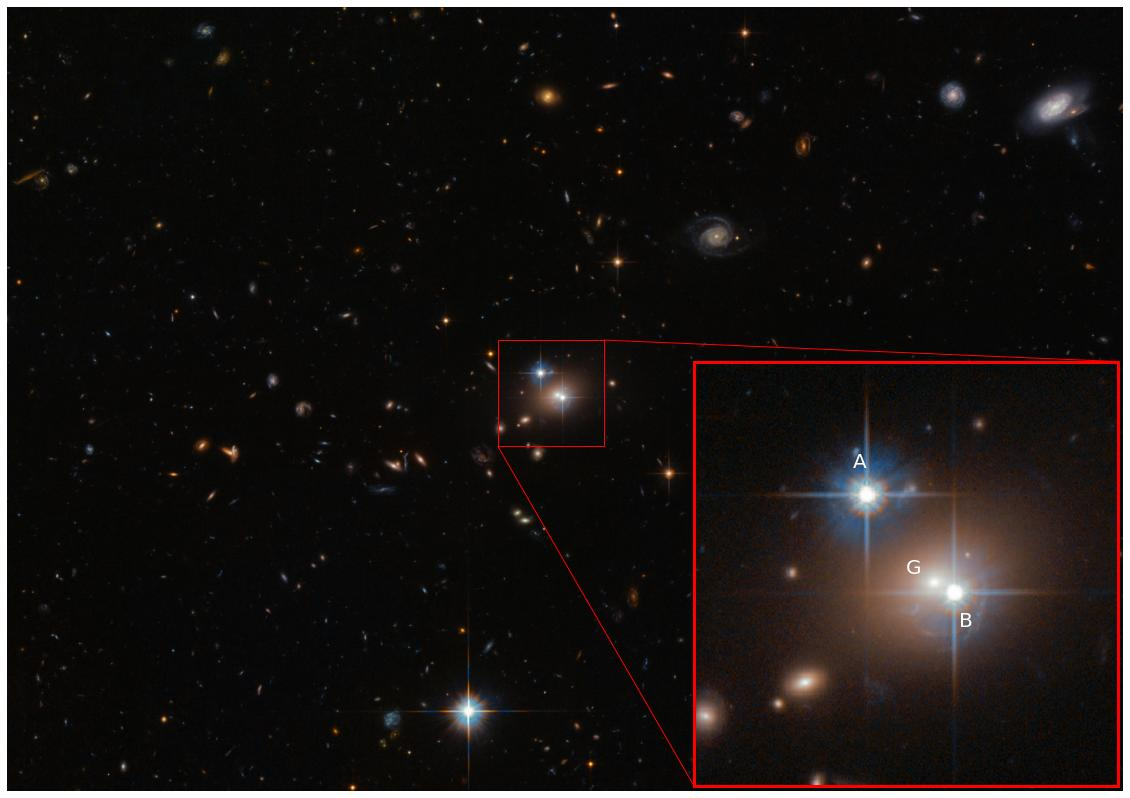
\includegraphics[width=0.8\textwidth]{figures/zoomed_in_qso0957}
        \caption{Le quasar double (QSO 0957+561 A et B) et la galaxie-lentille (G) imagé par le téléscope spatial Hubble. 
        Crédit: ESA/Hubble et NASA, enlargissement par AA.}
        \label{fig:doubel quasar}
\end{figure}

% Importance and difficuly of mass modelling
% For QSO, only 2 points and their relative magnitude can be used as constraint. Mass models has 5 params.
% Think about RXJ1131, which has a quad and we can see the galaxy in F814w -> importance to map the red and infra red!!

% Its relevance to cosmology

% Importance of source modelling and relevance to astrophysicd

% Lead up to next thing 
%L'importance des lentilles gravitationnelles 
%pour la cosmologie est subséquemment reconnue très tôt \citep[voir la revue de][]{Blandford1992}. 
%\begin{description}
        %\item[Cosmographie]
        %La cosmographie par délai temporelles \citep{Treu2016td,Suyu2017} permet en particulier de contraindre 
                %la constante de \citet{Hubble1929}, $H_0$, qui mesure le taux de l'expansion de l'Univers au temps présent. Les deux principales méthodes 
                %pour faire cette mesure sont la caractérisation de la courbe de lumière des supernovae \citet{Refsdal1964}, 
                %ç.-à-d. lentillé par une ou plusieurs galaxies \citep[e.g.][]{Kelly2015,Goobar2017}, et la surveillance décennale de quasars lentillés 
                %\citep[e.g.][]{Vanderriest1989,Wong2020};
        %\item[Inférence de la masse] Caractériser précisément les angles de déflections d'une lentille gravitationnelles permettent, en principe, 
                %d'inférer la distribution de masse
%\end{description}
%\begin{enumerate}
        %\item La cosmographie par délai temporelles \citep{Treu2016td,Suyu2017} En particulier, le paramètre le mieux contraint est 
                %la constante de \citet{Hubble1929} $H_0$, mesurant le taux de l'expansion de l'Univers au temps présent. Les deux principales méthodes 
                %pour faire cette mesure sont la caractérisation de la courbe de lumière des supernovae \citet{Refsdal1964}, 
                %ç.-à-d. lentillé par une ou plusieurs galaxies \citep[e.g.][]{Kelly2015,Goobar2017}, et la surveillance décennale de quasars lentillés 
                %\citep[e.g.][]{Vanderriest1989,Wong2019};
        %%\item Inférer la distribution de masse de la lentille pour une galaxie, ou un groupe de galaxie, et caractériser la distribution/présence 
                %%de matière noire, voir même de trous noirs supermassif ou de planètes ou étoiles extragalactiques (tdcosmos);
%%dark matter and its properties outside of the Milky Way \citep[e.g.,][]{Dala2002,Treu2004,Hezaveh2016,Gilman2020,Gilman2021}.
                %% Microlensing 
        %%\item De caractériser la structure de des protogalaxies dans l'Univers jeune, leur taux de formation d'étoiles et finalement 
                %%imager directement le disque d'accrétion de trous noirs supermassifs, soit le noyau actif de galaxies dans l'Univers jeunes;
        %%\item La recherche de plus de lentilles gravitationnelles et la caractérisation de leur propriétés de population pour l'inférence de 
                %%de choses comme l'évolution des galaxies relié à leur contenu de matière noir, alpha, etc.
        
%\end{enumerate}

%Cette découverte remarquable marque l'origine d'une ét
Le sujet de ce travail se concentre autour des lentilles gravitationnelles fortes de type galaxie-galaxie, e.g. QSO 0957+561. 
De tels systèmes sont caractérisé minimalement par une distortion de l'image source suffisamment forte pour causer 
l'apparition d'au moins deux images résolues de la source.
Pour une discussion plus général du phénomène, le lecteur peut se référer aux manuels de références par \citet{Meneghetti2013,Congdon2018} 
ou aux excellentes revues du sujet par \citet{Bartelmann2010,Treu2010}. 


%Une application importante de ces systèmes est l'étude du taux d'expansion de l'Univers 

%\subsection{Applications}
% Cosmologie - Image of RXJ1131 (mine) -> quasars
% Mass mapping + substructure detection (side mention of cluster and weak lensing) (constraints on dark matter?_
% Hierachecal studies (Ronan and previous paper Sonnenfeld etc)


%Il est intéressant de noter qu'\citet{Einstein1936} considérait la possibilité d'observer ce phénomène extrêmement improbable. En 
%fait, les calculs sont publiés 
%La résolution des télescopes optiques durant la majorité du XX\textsuperscript{e} siècle étaient 
%limités à environ $ 0.5$ arcsecondes par la turbulence de 
%l'air. Avec une telle résolution, un anneau d'Einstein d'une taille caractéristique de 1 arcseconde 
%apparaîtrait comme un point lumineux étalé, et ne serait donc pas distinguable d'une étoile. 

%Ce qu'il n'avait pas pris en compte c'est la possibilité de distinguer le spectre de l'objet 
%lentille à l'objet-lentille. En effet, comme ces objets se situent à deux redshift différent (pour un 
%système lentille observé en dehors du plan galactique de la Voie Lactée), alors il est possible en pratique 
%de détecter une lentille gravitationnelle simplement en analysant la raie spectrale du système. C'est de cette 
%façon que la première lentille gravitationelle fut découverte par \citet{Walsh1979} avec le téléscope radio Jodrell Bank MkIA. 
%Deux spectres identifiables à un rayonnement quasi-stellaire (quasar) presque identique, séparés de $5.7$ arcsecondes, 
%est la marque de la double image d'un seul quasar en arrière plan d'une galaxie. Dans ce cas particulier, le spectre de la 
%galaxie contamine légèrement le spectre de la contre-image du quasar, vu l'alignement imparfait. Il fallu quelques années 
%pour accepter ce résultat.

%Toutefois, cette première preuve expérimentale lanca le champ de recherche dans une nouvelle aire. L'étude du phénomène 
%s'est largement séparé en trois régime distinct: le régime micrométrique, le régime faible et le régime fort. Dans cette 
%étude, on s'intéresse principalement au régime fort, qui se distingue principalement des autres régime par le fait 
%que les déviations sont généralement de l'ordre de l'arcesecondes, de sortes qu'on peut observer les effet, et qu'on 
%distingue généralement plus d'une image de la source.

%Un autre direction de recherche, initiée par \citet{Refsdal1964}, est d'étudier l'évolution temporelle de supernovae lentillées 
%pour déterminer directement la constante de Hubble $H_0$, ou encore d'étudier, à une cadence de quelques jours entre chaque exposition, 
%un quasar lentillé plus d'une fois pour déterminer encore une fois la différence temporelle entre chaque image pour déterminer $H_0$.

%L'étude des effets de lentilles par les groups de galaxies est une discipline encore plus difficile que celle mentionnée jusqu'à maintenant, 
%dû à la complexité des profils de masses qui doivent être supposé et généralement dû à la difficulté de poser des contraintes qui requiert la mesure 
%de redshift de chaque images dans le champ de vue, et la présence de plusieurs sources différentes. On ne se concentre par sur cette étude, toutefois 
%on note que la recherche vers des algorithmes agnostiques sur le profil de marche est une avenue de recherche active dans cette discipline vu 
%la nécessité et aussi le genre de contraintes disponibles.

% Discovery of quasars in 1960
% First discovery of a grvaitational lens in 1979
% Explosion of their study -> models for the lens -> 2000s source reconstruction + H_0 motivations + cluster + others
% Saha 1997 first to try a full free-form reconstruction of galaxy-galaxy lens, his method has many limitations, requires strong regularisation and enormous hands-on fine-tuning 
% which makes the method hard to reuse / understand / caracterize its uncertainties
% Some free-form methods appear trying to correct error in the lensing potential of classical models for H_0. Then Birrer has his paper. 
% Explosion of machine learning in 2014. CNN are very efficient visual information processing tools. Laurence Yashar 2017
% Research in meta-learning lead to RIM (Putzky&Welling 2017), a general inverse problem solver that mimic traditional 
% gradient descent solver, but the prior is implicite, i.e. encoded as inductive biases in the neural network.
% Morningstar 2018/2019 use the method in the context of source reconstruction and interferometry reconstruction
% Our work.
% Context of our work
% Bulge-halo conspiracy, High SNR observation w/ JWST, Mass-sheet degeneracy?, Question is how to integrate information and use it properly
% Plan pour cette section: Dériver eq de la lentille et alpha
% Intro général: deflection de la lumière
%% Approcha a l'intro -> contexte historique à notre pensée sur la déviation de la lumière
%%% Réfraction 
%%%% Ptolémé (Optic, Grèce Antique)
%%%% Ibn Sahl (c. 940 - 1000)
%%%% Snell (1621)-Descartes(1637)
%%%% Principe de Fermat pour expliquer ce phénomène (lettre en 1657, mémoire en 1662)
%%%% Euler (1744) - Lagrange (1760) -> Principe de moindre action et sa solution
%%%% Équations de Maxwell (1861)

%%% déviation de la lumière par la gravité
%%%% Soldner, J. G. v. (1801–1804). "On the deflection of a light ray from its rectilinear motion, by the attraction of a celestial body at which it nearly passes by". Berliner Astronomisches Jahrbuch: 161–172.
%%%% Einstein 1911
%%%% Einstein 1915 (GR)
%%%% Eddington takes photograph of eclipse 1919
%%%% 1936 letter from Einstein at the request of 
%%%% Fritz Zwicky is first to postulate grav lensing idea in 1937i Zwicky, F. (1937) Nebulae as gravitational lenses. Physical Review, 51 (4). p. 290. ISSN 0031-899X
%%%% 1964 Refsdal (H0 and possibility to measure mass)
%%%%%% (Shapiro time delay (1964))
%%%% Fisrt gravitational lens discovered 1979 (double imaged quasar) https://www.nature.com/articles/279381a0
%%%% Then explosions of studies durings the 2000s on how to model things.

%%% Dark matter 
%%%% Zwicky 1933
%%%% Lambda CDM?
%%%% 

% Copied from https://royalsocietypublishing.org/doi/10.1098/rsta.2009.0209
%Henry Cavendish in 1784 is credited with the first (unpublished) calculation of the deflection angle 
%δ of a corpuscular light ray following a hyperbolic trajectory and the origin of the 
%(Newtonian) equation δ=2GM/Rc2. Subsequently, von Soldner (1804) published a similar calculation 
%deriving a deflection of 0.84 arcsec for stars viewed close to the limb of the Sun.

%Le principe de Fermat énonce que la trajectoire de la lumière, ou d'un 
%photon, doit suivre une trajectoire qui extrémise la durée de la trajectoire. 
%Ce principe mathématique, qui est un exemple du principe plus général de moindre action 
%développé par Lagrange en 1756, permet de décrire la trajectoire de la lumière 
%par l'entremise d'un simple indice $n$ (indice de réfraction) dans 
%lequel se cache toute la physique microscopique (ou macroscopique) 
%d'où émerge le phénomène qui nous intéresse. 


%L'expédition organisée par sir Arthur Eddington
%avait pour but d'observer 
%l'éclipse totale du 29 mai 1919 à partir de l'île de Prìncipe 
%dans le golfe de Guinée et de Sobral au nord du Brésil 
%\citep{Eddington1919}. Les photographes de l'éclipses prisent , bien qu'imprécises, 
%ont permis de valider la prédiction d'Einstein faite 
%en 1911 que la position observée d'une étoile serait déplacée de 
%$\delta \theta \approx 1.75'' \frac{R}{R_\odot}$ 
%durant une eclipse \citep{Dyson1920}, soit 2 fois plus 
%que ce qui est prédit par la théorie newtonienne.

%Dans l'intérêt de rendre ce manuscrit complet, je dérive à partir de principes 
%premier les deux équations centrales qui nous permettent 
%d'étudier les lentilles gravitationnelles.

\subsection{Les angles de déflections}
Dans les paragraphes qui suivent, je dérive les équations centrales qui nous permettent 
d'étudier les lentilles gravitationnelles de type galaxie-galaxie.
Mon traitement est largement inspiré 
des manuels de références de \citet{Meneghetti2013} et 
\citet{Carroll2003}.

Supposons qu'un photon est sur une trajectoire parallèle à l'axe de 
visée $\mathbf{e}_{\parallel}$ d'un observateur sur Terre. 
Supposons de plus que la source d'un champ gravitationnel $\Phi$ est situé sur l'axe de visée, 
ce qui a pour effet de courber la 
trajectoire de ce photon entre son point d'origine $A$ et son point d'arrivé $B$.
On définit l'angle de déviation comme la déviation totale de cette trajectoire 
dans la direction perpendiculaire à l'axe de visée de l'observateur. 
De façon générale, cette déviation s'écrit
\begin{equation}\label{eq:intro alpha}
        \boldsymbol{ \alpha} = - \int_{\lambda_A}^{\lambda_B} \ddot{\mathbf{x}} \times \mathbf{e}_{\parallel} d\lambda\, ,
\end{equation}
où $\lambda$ paramétrise la trajectoire du photon $\mathbf{x}(\lambda)$. 
Le signe négatif nous indique qu'on prend la perspective de l'observateur. 


%Pour résoudre l'intégrale \eqref{eq:intro alpha}, on doit déterminer la forme de 
%la trajectoire des photons dans un champ gravitationnel. Pour se faire, on faire usage du  
La trajectoire d'un photon est sujette au 
principe de Fermat, qui stipule que la lumière suit une trajectoire qui extrémise
la durée du parcours entre deux points. 
Dans le language du calcul 
des variations, la variation de la durée s'écrit
\begin{equation}\label{eq:Fermat}
        \delta T =  \delta \int_{A}^{B} n(\mathbf{x}(\ell)) \frac{d\ell}{c}= 0\, ,
\end{equation}
où $\ell$ est un élément de longueur sur la trajectoire et $n$ est un indice de réfraction.
Pour déterminer l'indice de réfraction du champ gravitationnel d'une galaxie, 
on doit utiliser le formalisme de la relativité générale. Selon le principe 
d'équivalence (fort), 
l'effet d'un champ gravitationnel est localement 
indistinguable d'une accélération causée par la courbure 
d'un espace-temps décrit par 
une métrique $g_{\mu \nu}$. 
La trajectoire d'un photon se trouve alors en cherchant 
les géodésiques de cet espace-temps. 
On fait l'approximation 
que le potentiel $\Phi$ d'une galaxie est celui d'un gas parfait, c'est-à-dire 
qu'il satisfait une équation de Poisson
\begin{equation}\label{eq:Poisson}
       \grad^{2}\Phi = 4\pi G \rho .
\end{equation} 
Dans la limite où ce potentiel est faible $\displaystyle \frac{2\Phi}{c^{2}} \ll 1$, la 
métrique $g_{\mu \nu}$ est décrite par une expansion au premier ordre autour de la 
métrique de Minkowsky %$\eta_{\mu\nu}$
\begin{equation}\label{eq:metrique}
        ds^2 = g_{\mu\nu}dx^{\mu}dx^{\nu} \approx \left( 1 + \frac{2\Phi}{c^{2}} \right)c^{2}dt^{2} - \left( 1 - \frac{2\Phi}{c^{2}} \right)d\mathbf{x}^{2}.
\end{equation} 
%Ici, j'ai choisit arbitrairement la signature $(+,-,-,-)$ pour la métrique.
Puisqu'un photon suit une géodésique de l'espace-temps $ds^{2} = 0$, on peut déterminer 
l'indice de réfraction en réarrangeant l'équation \eqref{eq:metrique}
\begin{equation}\label{eq:n}
        n \equiv c \left( \frac{\lVert d \mathbf{x} \rVert}{dt}  \right)^{-1} \approx  1 - \frac{2\Phi}{c^{2}}.
\end{equation} 
En réécrivant l'élément de longueur $d\ell$ en terme du 
paramètre de la trajectoire
$
        d\ell = \left\lVert\frac{d  \mathbf{x} }{d\lambda} \right\rVert d\lambda,
$
on peut réécrire l'équation \eqref{eq:Fermat} sous la forme
\begin{equation}\label{eq:Fermat2}
        \delta \int_{\lambda_A}^{\lambda_B} n(\mathbf{x}) \lVert \mathbf{\dot{x}} \rVert d\lambda = 0.
\end{equation} 
Par correspondance avec la fonctionnelle de l'action 
$J(x) = \int_{\lambda_0}^{\lambda_1} \mathcal{L}(\lambda,\, x,\,\dot{x}) d\lambda$ 
on trouve que 
le lagrangien de la trajectoire s'écrit 
$
        \mathcal{L} = n(\mathbf{x})  \sqrt{\dot{x}^{2}}.
$
La trajectoire qui satisfait \eqref{eq:Fermat} 
est une solution des équations d'Euler-Lagrange
\begin{equation}\label{eq:EulerLagrange}
        \frac{d }{d \lambda} \frac{\partial \mathcal{L}}{\partial \dot{\mathbf{x}}} - \frac{\partial \mathcal{L}}{\partial \mathbf{x}} = 0.
\end{equation} 
On a donc
\begin{equation}\label{eq:EulerLagrange2}
        \frac{d }{d \lambda} n \frac{\dot{\mathbf{x}}}{\lVert \dot{\mathbf{x}} \rVert}- \lVert \dot{\mathbf{x}} \rVert \grad n = 0 ,
\end{equation} 
Puisque le choix du paramètres $\lambda$ est libre, on peut le choisir tel 
que $\lVert \dot{\mathbf{x}} \rVert = 1$ en tout point de la trajectoire. Ainsi,
\begin{align}
        \nonumber
        \frac{d }{d \lambda} n \dot{\mathbf{x}} -  \grad n &= 0 \\
\label{eq:EulerLagrange3}
        \implies n \ddot{\mathbf{x}} + (\grad n \cdot \dot{\mathbf{x}}) \dot{\mathbf{x}} - \grad n &= 0
\end{align} 

À ce point de la dérivation, on utilise l'approximation de Born. 
C'est-à-dire qu'on approxime la trajectoire 
du photon comme une ligne droite sur l'axe de visée $\mathbf{e}_{\parallel}$. 
Cette approximation est justfiée 
dans le contexte des lentilles gravitationnelles de type galaxie-galaxie, 
puisque les angles de déviation sont généralement de 
l'ordre de l'arcseconde ou plus petit. 
Comme le vecteur $\dot{\mathbf{x}}$ est tangent à la trajectoire du photon, le 
terme $ \propto \dot{\mathbf{x}} \times \mathbf{e}_{\parallel} $ s'annule. 
En subsitutuant l'indice de réfraction par \eqref{eq:n} dans $\mathbf{e}_{\parallel} \times \eqref{eq:EulerLagrange3}$, on obtient
\begin{equation}\label{eq:sol}
        \ddot{\mathbf{x}} \times \mathbf{e}_{\parallel} = \frac{1}{n} \grad_\perp n = \grad_\perp \log n
        \approx -\frac{2}{c^{2}}\grad_{\perp} \Phi\,,
\end{equation} 
où $\grad_\perp$ est un gradient selon les coordonnées perpendiculaires à $\mathbf{e}_\parallel$.
On note que le facteur 2 qui apparaît dans l'équation \eqref{eq:sol} est un 
effet qui vient de la relativité générale. Ce facteur corrige la solution 
que l'on aurait obtenu avec une dérivation classique (newtonienne).


On est maintenant en mesure de calculer l'angle de déviation. 
J'introduit le paramètre d'impact $\boldsymbol{\xi}$ qui est la distance perpendiculaire entre 
la position d'origine du photon sur le plan de la lentille  
et l'axe de visé (voir Figure \ref{fig:cartoon}).
Dans le cas où le potentiel est généré par une masse $M$ ponctuelle, ç.-à-d.\ qu'on 
suppose $\rho = M\delta^{3}(\mathbf{x})$, où $\delta $ est la fonction delta de Dirac, 
alors le potentiel qui satisfait l'équation de Poisson \eqref{eq:Poisson} est 
la fonction de Green 
$\displaystyle \Phi = -\frac{GM}{\sqrt{ \xi^{2} + z^{2}}}$, où $z$ est la coordonné 
sur l'axe de visée. L'équation \eqref{eq:intro alpha} se réécrit finalement comme 
\begin{align}
\nonumber
        \boldsymbol{ \alpha}(\boldsymbol{ \xi} ) &= -\frac{2GM}{c^{2}} \int_{-\infty }^{\infty }  \frac{\partial}{\partial \boldsymbol{\xi} }\frac{1}{(\xi^{2} + z^{2})^{1/2}}dz \\
%\nonumber
        %&= \frac{2GM}{c^{2}} \boldsymbol{ \xi}  \int_{-\infty }^{\infty } \frac{1}{(\xi^{2} + z^{2})^{3/2}}dz  \\
\label{eq:deflection approx}
        \implies \boldsymbol{ \alpha}(\boldsymbol{ \xi})  &= \frac{4GM}{c^{2}  \xi^{2} } \boldsymbol{ \xi}
\end{align} 
Cette solution se généralise naturellement à un profil de masse quelconque en assumant 
qu'il s'exprime comme une somme d'élément de masses $dm = \Sigma d^{2}\boldsymbol{ \xi}'$, 
où $\Sigma = \int \rho dz$ est un densité surfacique de masse. 
L'angle de déviation total mesuré à un point $\boldsymbol{\xi} $ est alors une convolution 
sur tout le plan de la lentille (mince) puisque l'équation \eqref{eq:deflection approx} dépend 
linairement de la masse $M$:
\begin{equation}\label{eq:alpha physique}
        \boldsymbol{ \alpha} (\boldsymbol{ \xi} ) = \frac{4 G}{c^{2}} 
        \int_{\mathbb{R}^{2}} \Sigma (\boldsymbol{ \xi} ')
        \frac{\boldsymbol{ \xi}  - \boldsymbol{ \xi} '}{\lVert \boldsymbol{ \xi}  - \boldsymbol{ \xi} ' \rVert^{2}}d^{2}\boldsymbol{ \xi} '
\end{equation} 

L'angle de déviation est une quantité cruciale pour résoudre une lentille gravitationnelle 
puisqu'il décrit une transformation des coordonnées angulaires du plan de la lentille ($\boldsymbol{ \theta} $) 
vers les coordonnées angulaires du plan de la source ($\boldsymbol{ \beta} $). 
On assume que les distances entre l'observateur et la lentille $D_{\ell}$, entre l'observateur et la source $D_s$ et entre la lentille et la source $D_{\ell s}$, 
sont beaucoup plus grandes que les distances perpendiculaires à l'axe de visée $\boldsymbol{ \xi} $ ou $\boldsymbol{ \eta}$ 
(voir figure \ref{fig:cartoon}). 
Cette approximation est justifiée pour les objets qui nous intéresse,
pour lesquels les distances parallèles à l'axe de visée sont généralement 
de l'ordre du Gpc, alors que les distances perpendiculaire sont généralement 
de l'ordre du kpc; soit 6 ordres de grandeurs de différences.
Ainsi, on peut faire un argument géométrique (euclidien) 
\begin{align}
\nonumber
       D_{s} \boldsymbol{ \theta} &= \boldsymbol{ \eta}' \\   
\nonumber
       D_{s} \boldsymbol{ \beta} &= \boldsymbol{ \eta} \\   
\nonumber
       D_{\ell s} \boldsymbol{ \alpha} &= \boldsymbol{ \eta}' - \boldsymbol{ \eta}  \\   
\label{eq:lens equation}
       \implies D_s \boldsymbol{ \beta} &= D_s \boldsymbol{ \theta} - D_{\ell s} \boldsymbol{ \alpha}   
\end{align} 
La dernière relation est l'équation maîtresse qui nous permet de tracer les rayons lumineux d'une source 
vers un détecteur fictif dans nos simulations. On notera que cette relation reste valide pour un univers courbe et/ou en expansion 
(ç.-à-d.\ décrit par une géométrie non-euclidienne), 
à condition qu'on utilise une notion de distance qui satisfait, par définition, la relation trigonométrique euclidienne
\begin{equation}\label{eq:diameter angular distance}
       D \equiv \frac{\xi}{\theta}
\end{equation} 
où $\xi$ est la taille physique d'un objet placé à une certaine distance de l'observateur, et $\theta$ est l'angle solide sous-tendu 
par cet objet. Pour un Univers décrit par la métrique de Friedmann-Lemaître-Robertson-Walker,
la notion de distance qui respecte \eqref{eq:diameter angular distance} est la distance du diamètre angulaire. 
%Cette distance 
%prend en compte l'expansion de l'Univers et sa géométrie potentiellement courbe via la notion de distance comobile. 
En pratique, on peut s'exprimer directement cette distance en terme du décalage vers le rouge, $z$, des photons émis par l'objet
\citep[voir les manuels de référence][]{Bartelmann2004,Coles2002,Dodelson2003}
\begin{equation}\label{eq:diameter angular distance}%Bartelmann2004
        D_{z} = \frac{c}{H_0(1 + z)} \int_{0}^{z} \frac{dz'}{\sqrt{\Omega_{r,0} + \Omega_{m,0} (1 + z')^{-1}  + \Omega_{\Lambda,0}(1 + z')^{-4} + \Omega_{K}a(1 + z')^{-2}}}
\end{equation} 
où $\Omega_{r,0}$, $\Omega_{m,0}$ et $\Omega_{\Lambda, 0}$ sont les paramètres de densités au temps présent de la radiation, de la matière et l'énergie sombre 
respectivement. $\Omega_K = 1 - \Omega_0$ est le paramètre de courbure et $H_0$ est la constante de Hubble, soit le taux 
d'expansion de l'Univers au temps présent. 
%Dans le tableau \ref{tab:cosmos}, on donne la valeur des paramètres 
%du modèles cosmologique $\Lambda$CDM utilisé pour calculer \eqref{eq:diameter angular distance}. 
Par soucis de complétude, 
la valeur ajustée de ces paramètres par le téléscope Planck \citep{PlanckCollaboration2018}, 
pour le modèle cosmologique $\Lambda$CDM, est rapportée dans 
l'annexe \ref{app:lcdm}.

% Mettre en appendice
%\begin{table}[H]
        %\centering
        %\caption{Paramètres de $\Lambda$CDM ajusté avec les observations du fond diffus cosmologique par le téléscope Planck \citep{Planck2018}}
        %\label{tab:cosmos}
        %\begin{tabular}{cc}
                %\hline
                %Paramètre & Valeur \\\hline \hline
                %$\Omega_{r,0}$ & $\sim 10^{-4}$\\
                %$\Omega_{m,0}$  & 0.3158 \\
                %$h^{2}\Omega_{c,0}$  & 0.022383 \\
                %$\Omega_{b,0}h^{2}$ & 0.6842\\
                %$\Omega_{\Lambda,0}$ & 0.6842\\
                %$\Omega_{k}$ & $\equiv 0$\\
                %$h$ & $0.6732$ \\
               %\hline 
        %\end{tabular}
%\end{table}
%Avec le modèle cosmologique $\Lambda$CDM, cette équation se simplifie en 
%observant que l'Univers est plat et présentement dominé par la matière et l'énergie sombre, de sortes qu'on
 %calcule généralement la distance
%\begin{equation}\label{eq:diameter angular distance lcdm}
        %D^{\Lambda\mathrm{CDM}} = \frac{c}{H_0(1 + z)} \int_{z_2}^{z_1} \frac{dz'}{ \sqrt{\Omega_{m,0} (1 + z')^{-1}  + \Omega_{\Lambda,0}(1 + z')^{-4} }}
%\end{equation} 
%\begin{align*}
        %D &= c a(z_2) \int_{a(z_2)}^{a(z_1)} \frac{da}{a\dot{a}} \\
        %\dot{a}^{2} &= H_0^{2} \left[  \Omega_{r,0}a^{2} + \Omega_{m,0} a  + \Omega_{\Lambda,0}a^{-2} + \Omega_{k} \right] \\
        %H^{2} &= H_0^{2} \left[  \Omega_{r,0}a^{-4} + \Omega_{m,0} a^{-3}  + \Omega_{\Lambda,0} + \Omega_{K}a^{-2} \right]
%\end{align*}

Il est généralement pratique de travailler avec la forme adimensionnelle de l'équation \eqref{eq:lens equation}. 
On introduit la densité critique 
\begin{equation}\label{eq:densite critique}
        \Sigma_c = \frac{c^2}{4 \pi G}\frac{D_{s}}{D_{\ell s} D_\ell}\, ,
\end{equation} 
qui nous permet de définir la quantité qu'on nomme convergence $\displaystyle \kappa(\boldsymbol{ \theta} ) \equiv \frac{\Sigma(\boldsymbol{ \theta})}{\Sigma_c}$. 
On définit ainsi l'angle réduit 
\begin{equation}\label{eq:alpha adim}
        \hat{\boldsymbol{ \alpha}} (\boldsymbol{ \theta}) = \frac{1}{\pi}\int_{\mathbb{R}^{2}} \kappa(\boldsymbol{ \theta} )
        \frac{\boldsymbol{ \theta} - \boldsymbol{ \theta}'  }{\lVert \boldsymbol{ \theta} - \boldsymbol{ \theta}' \rVert  } d^{2}\boldsymbol{ \theta}'\, ,
\end{equation} 
qui satisfait l'équation de la lentille adimensionnelle 
\begin{equation}\label{eq:lens equation adim}
        \boldsymbol{ \beta} = \boldsymbol{ \theta} - \hat{\boldsymbol{ \alpha}}(\boldsymbol{ \theta})\, . 
\end{equation}

\begin{figure}[H]
        \centering
        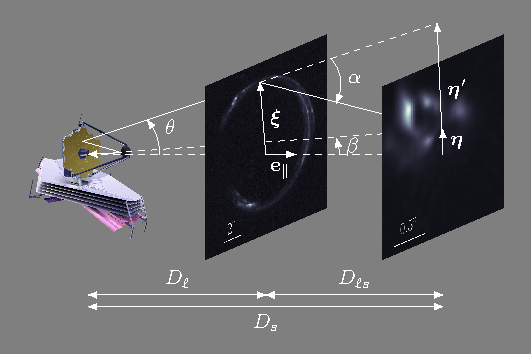
\includegraphics[width=0.8\textwidth]{figures/lensing_cartoon}
        \caption{Schéma d'une lentille gravitationnelle.}
        \label{fig:cartoon}
\end{figure}


% 




%Strong gravitational lensing is a natural phenomenon through which multiple distorted images of luminous background objects, 
%i.e. early-type star-forming galaxies, are formed by massive foreground objects along the line of sight 
%\citep[e.g.,][]{Viera2013,Marrone2018,Rizzo2020,Sun2021}. 
%These distortions are tracers of the distribution of mass in foreground objects, independent of the electromagnetic behaviour of these overdensities. 
%As such, this phenomenon offers a powerful probe of the distribution of 
%dark matter and its properties outside of the Milky Way \citep[e.g.,][]{Dala2002,Treu2004,Hezaveh2016,Gilman2020,Gilman2021}.

%Lens modeling is the process of inferring the parameters describing both the mass distribution in the 
%foreground lens and undistorted image of the background source.
%This has traditionally been a time- and resource-consuming procedure. 
%A common practice to model the mass of lensing galaxies is 
%to assume that their density profiles 
%follow simple parametric forms, e.g., a power law $\rho \propto r^{-\gamma'}$. 
%These profiles generally provide a good fit to low-resolution data and are easy to work with due to their small number of parameters \citep[e.g.,][]{Koopmans2006,Barnabe2009,Auger2010}. 
%However, as high-resolution and high signal-to-noise ratio (SNR) images become available, lens analysis with simple models requires the introduction of additional parameters representing the true complexity of the mass distribution in lensing galaxies and their immediate environments \citep[e.g.,][]{Sluse2017,Wong2017,Birrer2019,Rusu2019, Rusu2017,Li2021}. 
%This approach becomes intractable as the quality of images increases. For example,
%no simple parametric model of the Hubble Space Telescope (HST) Wide Field Camera 3 (WFC3) images of 
%the Cosmic Horseshoe (J1148+1930) --- initially discovered by \citet{Belokurov2007} --- 
%has been able to model the fine features of the extended arc 
%\citep[e.g., ][]{Bellagamba2016,James2018,Cheng2019,Schuldt2019}.

%Free-form methods --- also misleadingly called nonparametric methods ---
%attempt to relax the assumptions about the smoothness and symmetries of these parametric profiles 
%by changing their parametric support to more expressive families like regular (or adaptive)
%grid representations and meshfree representations. 
%But, this added flexibility comes at a price, which is (often) a high-dimensional inference problem that is under-constrained, meaning that imposing a prior on the reconstructed parameters becomes essential to penalize unphysical solutions and avoid overfitting the data. 
%% \citep{Bartelmann1996,Saha1997,Seitz1998,Abdelsalam1998,Abdelsalam1998b,Diego2005,Diego2007,Liesenborgs2006,Liesenborgs2007,Coe2008,Merten2009,Birrer2015,Merten2016,Torres-Ballestros2022}. 
% Kaiser And Squires Mass mapping weak lensing (leading up to Remy2022 - score based method reinforcing results from deep learning obtain 2 year prior by same group, and other method cited in this paper)
% Bartelmann 1996 (cluster lensing free-form reconstruction, with a priori known 10^5 galaxy source as background -> reconstruct potential starting from smoothed prior)
% Abdelsalam et al. (1998)
% Saha & Williams (1997)
% Seitz & Schneider (1998) Maximum entropy regularisation (cluster lensing, free-form inversion of the kappa map)
% Cacciato, Bartelmann 2006 -> combine weak and strong lensing info in cluster to reconstruct 2d potential, focus on using arcs to constrain the location of critical curves (very similar to Bradac work, except this critical curve thing)
% Jee et al 2007: Discovery of a ring-like dark matter structure in the cluster  Cl 0024+17 (pretty cool)
% Deb, Goldberg 2008: Particle Based Lensing, used for cluster reconstruction, can include all information like weak lensing, strong lensing constraints (image positions, flux, known position of critical curves)
% Liesenbourg (2006, -07, -09, -20): GRALE, genetic algorithm to infer kappa for cluster lensing by summing over basis function (Plummer profiles)
% Gosh et al 2020: GRALE can reconstruct cluster with up to 1000 multiple images for ultra deep fields images of certain clusters (e.g. w/ JWST)
% Diego et al 2005, 2007: WSLAP - probably the only method using pixel with no known arcs to constrain further the free-form mass model (mutliresolution grid parameter family)
% Bradac 2005a,b and 2009: SWUnited: combine weak and strong lensing info to break the mass sheet degeneracy for cluster lensing
% Coe et al 2008: LensPerfect - perfect reproduction of image position, flux and shear for cluster lenses. Explore thoroughly analytical priors for mass maps etc.
% Mertens 2009, -11, -16 SaWLens, 2009 explore the introduction of regularisation into the Weak + Strong lensing constraints, 2011: application to real data, 2016: mesh-free reconstructions.
%Free-form methods have a rich history in cluster-scale lensing \citep{Bartelmann1996,Seitz1998,Abdelsalam1998,Abdelsalam1998b,Bradac2005,Diego2005,Cacciato2006,Diego2007,Liesenborgs2006,Liesenborgs2007,Jee2007,Coe2008,Merten2009,Deb2012,Merten2016,Ghosh2020,Torres-Ballestros2022} and weak lensing \citep{Kaiser1993,Marshall2001,Massey2007,Deb2008,Simon2012,Leonard2012,Lanusse2016,Jeffrey2020,Starck2021,Remy2022}. They strive to make better use of the information contained in lensing features like resolved arc details, multiple image position, flux ratios, image deformation (i.e. weak lensing constraints) or even the null space of an image in order to place better constraints on the morphology of the mass density of the lens.
%On the other hand, comparatively less work has been done in the context of galaxy-galaxy lensing system to tackle free-form mass modelling directly \citep{Saha1997,Saha2004,Birrer2015,Coles2014}. The main reason for this state of affairs is the difficulty of specifying an appropriate prior which regularizes the problem over its non-linear parameters while maintaining computational tractability and sufficient flexibility to model a large variety of systems. 

% However, while these higher-dimensional parameter spaces add flexibility to the model, 
% exploring this complex multimodal space with traditional non-linear optimizers becomes quickly computationally intractable. 
% However, the price to pay for the flexibility of the free-form methods is (often) a high-dimensional inference problem that is under-constrained, meaning that imposing a prior on the reconstructed parameters becomes essential to penalize unphysical solutions and avoid overfitting the data. 

%In view of this, the focus of the field has instead been on using free-form methods for the background source reconstruction only. 
%A number of well-established procedures exists for linear inversion of pixellated-source models  in the context of traditional maximum likelihood modeling. These methods, originally developed by \citet{Warren2003,Suyu2006}, are based mainly on imposing a quadratic-log prior to the source pixels to regularize the optimisation. Subsequently, there have been multiple attempts at building a bridge toward free-form methods in order to correct simplistic assumptions on the mass density model by using linear corrections of the lensing potential \citep{Koopmans2005,Suyu2006b,Vegetti2009,Vegetti2012}, or iteratively specified priors for shapelets corrections \citep{Birrer2018,Nightingale2018}. But these extensions are generally limited by assumptions regarding the accuracy of the initial parametric models, and thus we are left wanting for a more flexible approach. 
% Despite this, the problem of developing a fully fledged method for a free-form mass density reconstruction algorithm in the context of galaxy-galaxy lensing remains open. 
% Many choices of priors are too constraining. overall this is a really hard problem, and it's so computationally expensive and degenerate that we can't test or characterize any of those models for systematics, let alone investigate ways correct for them.

%Over the recent years, deep learning methods have proven extremely successful at modeling quickly and accurately strong lensing systems \citep{Hezaveh2017,PerreaultLevasseur2017,Morningstar2018,Coogan2020,Park2021,Legin2021,Wagner-Carena2021,Schuldt2022,Wagner-Carena2022,Karchev2022,AnauMontel2022,Mishra-Sharma2022}.
%More specifically, \citet{Morningstar2019} demonstrated that recurrent convolutional neural networks can learn implicitly complex prior distributions from their training data to successfully reconstruct pixelated undistorted images of strongly lensed sources, circumventing the need to specify explicitly a prior distribution over those parameters. Motivated by this success, we propose a method that extends this framework to solve the full lensing problem and simultaneously reconstruct a pixelated lensing mass map and a pixelated undistorted background source.

%In this work, we propose a method for pixelated 
%strong gravitational lensing mass and source reconstruction, 
%allowing it to reconstruct complex distributions. 
%The method we propose here is based on the Recurrent Inference Machine (thereafter refered to as RIM), originally developed by \citet{Putzky2017}. 
%In this framework, we aim to learn an iterative inference algorithm, moving away 
%from hand-chosen inference algorithms and hand-crafted priors. 
%Instead, the prior is learned implicitly through the dataset used to train 
%the neural network that update the solution parameters at each iteration. 


\section{Interférométrie par masque non-régulier}

%\subsection{Contexte historique}

\subsection{Les angles de fermeture}

\subsection{Applications}


\section{Auto-encodeur variationnel}

\subsection{Description du modèle}

Les auto-encodeurs variationnels (VAE) ont été introduits par \citet{Kingma2013} comme une approche 
pour inférer approximativement les variables latentes (ou cachées) qui modélisent une distribution 
a posteriori définie implicitement via un échantillon de données. Dans cette section, j'introduis 
les concepts principaux relié à ce type de modélisation. 
Le lecteur peut aussi se référer au livre blanc de \citet{Kingma2019}.

On définit $\mathbf{z}\in \mathbb{R}^{h}$ comme une variable latente et $\mathbf{x}\in \mathbb{R}^{m}$ ($m > h$) 
comme un example d'un échantillon de donnée $\mathcal{D} = \{\mathbf{x}^{(i)}\}_{i=1}^{N}$. 
Notre objectif est de modéliser la distribution, $p(\mathbf{x})$, implicitement décrite par notre échantillon. 
On définit une approximation de cette distribution, $p_\theta(\mathbf{x})$, caractérisée par une liste de paramètres $\theta$,
et on définit un processus génératif modélisé par la conditionnelle sur la variable cachée $p_\theta(\mathbf{x \mid \mathbf{z}})$. 
Déterminer $p_\theta$ est généralement difficile, voir intraitable, si la dimensionalité de $\mathbf{x}$ est grande 
($\mathrm{dim(\mathbf{x}}) \gtrsim 10^{4}$ pour des images). 
On introduit donc une distribution variationnelle, $q_\phi(\mathbf{z} \mid \mathbf{x})$, dont le rôle est de 
d'inférer la variable latente $\mathbf{z}$ associé à $\mathbf{x} \sim p_\theta(\mathbf{x} \mid \mathbf{z})$. 
En d'autres mots, $q_\phi(\mathbf{z} \mid \mathbf{x})$ est une approximation variationnelle de la distribution a posteriori $p_\theta(\mathbf{z} \mid \mathbf{x})$.
%\begin{equation}\label{eq:vae 1}
        %q_\phi (\mathbf{z} \mid \mathbf{x}) \approx p_\theta (\mathbf{z} \mid \mathbf{x})\, .
%\end{equation} 
La notion de distance entre ces deux distributions est mesurée par la divergence de Kullback-Leibler $D_{\mathrm{KL}}(\cdot \KL \cdot) \geq 0$: 
\begin{align}
        \nonumber
       D_{\mathrm{KL}}(q_\phi(\mathbf{z} \mid \mathbf{x}) \KL  p_\theta (\mathbf{z} \mid \mathbf{x})) 
       &= \mathbb{E}_{q_\phi(\mathbf{z} \mid \mathbf{x})} \bigg[\log q_\phi(\mathbf{z} \mid \mathbf{x}) - \log p_\theta (\mathbf{z} \mid \mathbf{x}) \bigg]  \\
       \nonumber
       &= \mathbb{E}_{q_\phi(\mathbf{z} \mid \mathbf{x})} \bigg[\log q_\phi (\mathbf{z} \mid \mathbf{x}) -\log \frac{p_\theta(\mathbf{z}, \mathbf{x})}{p_\theta(\mathbf{x})} \bigg]  \\
       \label{eq:KL}
       &= \log p_\theta (\mathbf{x}) - \underbrace{\mathbb{E}_{q_\phi(\mathbf{z} \mid \mathbf{x})} \bigg[\log p_\theta(\mathbf{z}, \mathbf{x}) - \log q_\phi (\mathbf{z} \mid \mathbf{x}) \bigg]}_{\equiv \mathcal{L}_{\phi,\theta}(\mathbf{x})} \, .
\end{align} 

On remarque par cette manipulation que la distance $D_{\mathrm{KL}}$, en plus de mesurer la distance entre 
les deux distributions a posteriori (par définition), mesure aussi la différence entre le terme 
$\mathcal{L}_{\phi,\theta}(\mathbf{x})$, qu'on nomme limite inférieure sur l'évidence (de l'anglais 
\textit{evidence lower bound}: ELBO), et la distribution marginale qu'on cherche à modéliser, $p_\theta(\mathbf{x})$. 
L'objectif d'un modèle VAE est de maximiser la ELBO, $\mathcal{L_{\phi,\theta}}$. 
En observant l'équation \eqref{eq:KL}, on réalise que 
que ceci accomplit deux objectifs simultanément qui suivent du fait que la divergence KL est 
une quantité positive:
\begin{enumerate}
        \item Améliorer le processus génératif puisque $p_\theta(\mathbf{x}) = \int p_{\theta}(\mathbf{x} \mid \mathbf{z}) p_{\theta}(\mathbf{z}) d\mathbf{z}$ 
                est maximisé, ce qui suit de l'inégalité
                $\log p_\theta \geq \mathcal{L}_{\phi,\theta}(\mathbf{x})$;
        \item Améliorer le processus d'inférence puisque 
        $D_{\mathrm{KL}}(q_\phi(\mathbf{z} \mid \mathbf{x}) \KL  p_\theta (\mathbf{z} \mid \mathbf{x})) = \log p_\theta(\mathbf{x}) - \mathcal{L}_{\phi,\theta}(\mathbf{x})$ est simultanément minimisé.
\end{enumerate}

\begin{figure}[H]
        \centering
        \begin{tikzpicture}
                \node[circle, draw=black, minimum size=1cm] (z) at (0, 3) {$\mathbf{z}$};
                \node[circle, draw=black, minimum size=1cm] (x) at (0, 0) {$\mathbf{x}$};
                \draw[-{Latex[scale=2]}] (z) to (x);
                \draw[-{Latex[scale=2]}, in=225, out=135, dashed] (x) to (z);
                \node (phi) at (-2.5, 2.5) {$\phi$};
                \node (theta) at (2.5, 2.5) {$\theta$};
                \draw[rounded corners=0.5cm] (-1.5, -0.7) rectangle (1.5, 3.7);
                \draw[-{Latex[scale=2]}] (theta) to node[sloped, midway, below=5pt, fill=white, rectangle, draw=white, opacity=.8, text opacity=1] {$p_\theta(\mathbf{\mathbf{x} \mid \mathbf{z}})$} (x);
                \draw[-{Latex[scale=2]}] (theta) to node[sloped, midway, above=5pt, fill=white, rectangle, draw=white, opacity=.8, text opacity=1] {$p_\theta(\mathbf{z})$} (z);
                \draw[-{Latex[scale=2]}, dashed] (phi) to node[sloped, midway, above=5pt, fill=white, rectangle, draw=white, opacity=.8, text opacity=1] {$q_\phi(\mathbf{z} \mid \mathbf{x})$} (z); 
                \node at (1, -0.5) {$N$};
        \end{tikzpicture}
        \caption{Modèle graphique d'un VAE. Les flèches pleines indiquent le processus génératif, alors que les flèches pointillées indiquent le processus d'inférence.}
        \label{fig:vae encoder}
\end{figure}

\subsection{Le truc de reparamétrisation}
Le gradient de la ELBO par rapport aux paramètres variationnels, $\grad_{\phi,\theta}\mathcal{L}_{\phi,\theta}(\mathbf{x})$, 
est une quantité qu'on doit calculer pour faire usage d'algorithmes comme la grimpe de gradient stochastique 
pour maximiser la ELBO en terme de $\phi$ et $\theta$. 
Or, la liste de paramètres $\phi$ apparait dans la distribution de prélevement pour calculer 
l'espérance mathématique $\mathbb{E}_{q_\phi(\mathbf{z} \mid \mathbf{x})}$ dans la ELBO \eqref{eq:KL}.
Cette opération n'a pas de dérivée formelle en terme de $\phi$. 

Pour résoudre ce problème, on utilise le truc de reparamétrisation \citep{Kingma2013}, 
qui consiste à exprimer la variable aléatoire latente $\mathbf{z} \sim q_\phi (\mathbf{z} \mid \mathbf{x})$ 
comme la transformation différentiable et inversible d'une variable aléatoire auxiliare $\boldsymbol{\epsilon}$.
On considère le cas où $q_\phi(\mathbf{z} \mid \mathbf{x})$ et $p(\boldsymbol{ \epsilon})$ 
font partie de la famille gaussienne isotropique
\begin{align}
        \label{eq:p epsilon}
        \boldsymbol{\epsilon} &\sim \mathcal{N}(0, \bbone)\, ;\\
        %\label{eq:q phi}
        %q_\phi(\mathbf{z} \mid \mathbf{x}) &= \mathcal{N}(\boldsymbol{ \mu}_\phi (\mathbf{x}),\, \bbone \boldsymbol{\sigma}_\phi^{2}(\mathbf{x}))\, ;\\
        \label{eq:reparametrisation}
        \mathbf{z} &= \boldsymbol{\mu}_\phi + \boldsymbol{ \sigma}_\phi \odot \boldsymbol{ \epsilon}\, , 
\end{align} 
de sortes que 
\begin{equation}\label{eq:q phi}
        \mathbf{z} \sim q_\phi(\mathbf{z} \mid \mathbf{x}) = \mathcal{N}(\boldsymbol{ \mu}_\phi (\mathbf{x}),\, \bbone \boldsymbol{\sigma}_\phi^{2}(\mathbf{x}))\, .
\end{equation} 
$\odot$ symbolise le produit d'Hadamard, ou encore le produit élément-par-élément de vecteurs.
La reparamétrisation fait en sortes que les paramètres variationnelles ne participent plus au procsessus de prélevement, 
maintenant pris en charge par $\boldsymbol{ \epsilon} $.
Cette propriété est cruciale, car elle nous permet de prendre le gradient de la ELBO \eqref{eq:KL}. 
En effet, on peut maintenant échanger les opérateurs $\grad_{\phi,\theta}$ et ${\mathbb{E}_{q_\phi(\mathbf{z} \mid \mathbf{x})} = \mathbb{E}_{p(\boldsymbol{ \epsilon})}}$,
ce qui nous permet d'appliquer le gradient à l'intérieur de l'espérance mathématique.
De plus, $\phi$ décrit maintenant une fonction générique dont le rôle est d'inférer les 
paramètres de la distribution $q_\phi(\mathbf{z} \mid \mathbf{x})$
\begin{equation}\label{eq:}
        \begin{aligned}
                f_\phi: \mathbb{R}^{m} &\rightarrow \mathbb{R}^{h} \times \mathbb{R}^{h}\\ \mathbf{x} &\mapsto (\boldsymbol{\mu},\, \log \boldsymbol{\sigma}^{2})
        \end{aligned}
\end{equation} 
En pratique, on peut construire une approximation de 
cette fonction avec un réseau de neuronnes convolutionnelles lorsque $\mathbf{x}$ est une image, 
suivant le principe d'approximation universelle \citep{Cybenko1989,Hornik1991}. 

L'objectif d'entraînement de la fonction $f_\phi$ nécessite de manipuler la ELBO pour obtenir une 
divergence KL
\begin{align}
        \mathcal{L}_{\phi,\theta}(\mathbf{x}) &= \mathbb{E}_{q_\phi(\mathbf{z} \mid \mathbf{x})} \bigg[ \log p_\theta(\mathbf{z}, \mathbf{x}) - \log q_\phi (\mathbf{z} \mid \mathbf{x}) \bigg]\, ; \\
        \label{eq:final elbo}
         \implies \mathcal{L}_{\phi,\theta}(\mathbf{x})  &= 
         \underbrace{\mathbb{E}_{q_\phi(\mathbf{z} \mid \mathbf{x})} \bigg[ \log p_\theta(\mathbf{x} \mid \mathbf{z})\bigg]}_{\text{terme de reconstruction}}
         + \underbrace{
                \mathbb{E}_{q_\phi(\mathbf{z} \mid \mathbf{x})} \bigg[\log p_{\theta}(\mathbf{z}) - \log q_\phi (\mathbf{z} \mid \mathbf{x}) \bigg]
        }_{\equiv -D_{\mathrm{KL}}(q_\phi(\mathbf{z} \mid \mathbf{x})\, \KL\, p_\theta(\mathbf{z}))}\, .
\end{align} 
Pour déterminer la forme fonctionnelle de la divergence KL obtenue au second terme du membre droit de l'équation \eqref{eq:final elbo}, 
on stipule a priori que la distribution marginale des variables latentes 
devrait correspondre à une distribution normale isotropique
\begin{equation}\label{eq:latent distribution}
        p_{\theta}(\mathbf{z}) = \mathcal{N}(0, \bbone)
\end{equation}
On est libre de faire ce choix sans pour autant limiter les formes possibles de la distribution qui nous intéresse $p_\theta(\mathbf{x})$.
%On peut alors exprimer la ELBO comme
%La divergence de KL obtenue au second terme du membre droit de l'équation \eqref{eq:final elbo} 
La KL admet alors une solution fermée étant donné les familles paramétriques stipulées 
pour $p_\theta(\mathbf{z})$ \eqref{eq:latent distribution} et $q_\phi(\mathbf{z} \mid \mathbf{x})$ \eqref{eq:q phi}
\begin{equation}\label{eq:final KL}
        -D_{\mathrm{KL}}(q_\phi(\mathbf{z} \mid \mathbf{x})\, \KL\, p_\theta(\mathbf{z})) =
        \frac{1}{2}\sum_{j=1}^{\mathrm{dim}(\mathbf{z})} (1 + [\log \boldsymbol{ \sigma}_\phi^{2} ]_j - [\boldsymbol{ \mu}_\phi ]_j - [\boldsymbol{ \sigma}_\phi^{2} ]_j)
\end{equation} 
Une dérivation de ce terme est donnée dans l'appendice B de \citet{Kingma2013}. 
%Cette solution se dérive directement par rapport à $\phi$. 
Le premier terme du membre droit de l'équation \eqref{eq:final elbo} 
est nommé \textit{terme de reconstruction} puisqu'il connecte avec l'objectif des fonctions 
de type auto-encodeurs d'apprendre une représentation latente d'un échantillon de données.
La reconstruction s'accomplit en utilisant d'abord le modèle d'inférence 
$\mathbf{z}^{(1:L)} \overset{\mathrm{i.i.d}}{\sim} q_\phi(\mathbf{z} \mid \mathbf{x})$ 
pour obtenir un échantillon de représentations latentes à partir des équations \eqref{eq:p epsilon} à \eqref{eq:reparametrisation}, 
puis en utilisant le modèle génératif $\hat{\mathbf{x}}^{(i)} \sim p_\theta(\mathbf{x} \mid \mathbf{z}^{(i)})$ pour obtenir 
un échantillon de reconstructions $\mathbf{\hat{x}}^{(1:L)}$ similaire à l'exemple originel $\mathbf{\mathbf{x}}$. 
Comme on a déjà une variable auxiliaire $\boldsymbol{ \epsilon} $ 
qui se charge de l'aspect génératif du modèle, on peut construire une approximation du 
modèle génératif avec une fonction générique des variables latentes 
${g_\theta: \mathbb{R}^{h} \rightarrow \mathbb{R}^{m};\, \mathbf{z}^{(i)} \mapsto \hat{\mathbf{x}}^{(i)}}$.
Encore une fois, un réseau de neuronnes convolutionnelles est un choix pratique pour modéliser cette fonction 
dans le cas où $\mathbf{x}$ est une image. En général, on choisit une erreur quadratique moyenne pour modéliser le terme de reconstruction, 
de sorte que
\begin{equation}\label{eq:reconstruction}
        \mathbb{E}_{q_\phi(\mathbf{z} \mid \mathbf{x})} \bigg[
                \log p_\theta(\mathbf{x} \mid \mathbf{z})
        \bigg] 
        \simeq -\frac{1}{L}\sum_{i=1}^{L} \lVert \mathbf{x} - \hat{\mathbf{x}}^{(i)} \rVert_2^{2}
\end{equation} 

Je note que la fondation théorique des auto-encodeurs variationnels repose sur le principe plus général 
du goulot d'information \citep{Tishby1999}; un sujet qui n'est pas abordé dans ce travail, mais qui motive 
l'utilisation de la version $\beta$-VAE du modèle esquissé dans cette section. Sans rentrer dans les détails, on note 
qu'il est possible de dériver l'objectif de notre auto-encodeur via la théorie de l'information de \citet{Shannon1948} en interprétant 
l'auto-encodeur comme un système de transmission d'information par compression, avec perte. 
Une approche naïve pour modéliser ce système serait de maximiser le taux d'information transmise par le système, 
ç.-à-d. que le nombre de bit moyen encodé dans une variable latente aléatoire $Z$, mesuré par l'information 
mutuelle entre le message $X$ et le code $Z$ utilisé pour représenter le message $I(X; Z)$, devrait se rapprocher 
d'un maximum qu'on nomme la capacité du système $C = \underset{P(X)}{\mathrm{max}}\, I(X;\,Z)$. 
Toutefois, cet objectif ne mentionne rien sur la qualité ou la pertinence de cette information. Pour obtenir un message pertinent, 
on veut contraindre la complexité de Kolmogorov du message, ce qui peut être accomplit en contraingnant le code $Z$
à utiliser le moins de bit possible pour encoder le message. 
C'est le principe de base de la théorie du taux de distortion \citep{Cover2006}. 
\citet{Tishby1999} observe que la mesure du taux de distortion suivante 
\begin{equation}\label{eq:bottleneck principle}
        \mathcal{L}\left[ p(\hat{\mathbf{x}} \mid \mathbf{x}) \right]  = I(\hat{X}; X) - \beta I(\hat{X};Z)
\end{equation}
%permet d'atteindre un compromis entre les deux objectifs qui nous interesse, soit des reconstruction de haute qualité 
%et une compression informative (ç.-à-d. minimale).
Le paramètre $\beta$ est un multiplicateur de Lagrange qui contrôle le niveau de compression désiré
%\citet{Tishby2000} observe que cet objectif ne contraint pas la qualité ou la pertinence de cette information. La théorème , mais plutôt 
%où un multiplicateur de Lagrange vient multiplier la distance KL dans la ELBO.
Le lecteur est invité à se référer à la revue sur le sujet par \citet{Goldfield2020}.

\section{Machines à inférence récurrentielles}
\subsection{Formalisme bayésien des problèmes inverses}

Les machines à inférence récurentielles (RIM) ont été introduites par \citet{Putzky2017} pour résoudre des problèmes 
inverses pour lesquels le terme de régularisation est nécessaire mais inconnue a priori et/ou difficile à 
construire, voir même calculer. Dans cette section, j'introduis le formalisme bayésien des problèmes inverses sur lequel 
ce modèle repose, puis j'introduis l'algorithme d'inférence et les concepts d'apprentissage machine qui motivent 
l'utilisation d'une RIM pour des problèmes inverses mal-posés et sous-déterminés.

Les problèmes inverses en astrophysique prennent généralement la forme
\begin{equation}\label{eq:inverse problem lineaire}
       \mathbf{y} = F(\mathbf{x}) + \boldsymbol{\eta}\, ,
\end{equation} 
où $\mathbf{y}\in \mathcal{Y}$ est un vecteur d'observables (comme l'image capturé par les capteurs photographiques CCD dans un téléscope), 
$\mathbf{x}\in\mathcal{X}$ est un vecteur de paramètres qui gouvernent le phénomène physique qui nous intéresse, 
modélisé par le modèle physique $F:\mathcal{X} \rightarrow \mathcal{Y}$.
Le vecteur $\boldsymbol{\eta}$ est une réalisation d'un bruit additif. 
On suppose qu'on connait la distribution de ce bruit, de sortes qu'on peut modéliser la fonction de vraisemblance de l'observable
\begin{equation}\label{eq:likelihood intro}
        \mathbf{y} - F(\mathbf{x}) \sim p(\boldsymbol{ \eta}) = p(\mathbf{y} \mid \mathbf{x})\, .
\end{equation} 
Le problème d'inférence est celui de déterminer les paramètres $\mathbf{x}$ qui reproduisent l'observation $\mathbf{y}$, 
ç.-à-d. l'estimé des paramètres $\hat{\mathbf{x}}_{\mathrm{MLE}}$ 
qui maximisent la fonction de vraisemblence (MLE de l'anglais \textit{maximum likelihood estimate}), 
ou de façon équivalente ceux qui maximisent le log de la vraisemblence
\begin{equation}\label{eq:likelihood max}
        \hat{\mathbf{x}}_{\mathrm{MLE}} = \underset{\mathbf{x} \in \mathcal{X}}{\mathrm{argmax}}\, \log p(\mathbf{y} \mid \mathbf{x})\, .
\end{equation} 
Dans le cas général, ce problème est mal posé et n'a pas de solutions. En effet, 
tel que l'observe \citet{Hadamard1902}, un problème aux dérivée partielles comme \eqref{eq:likelihood max} 
ne possède une solution que si le problème est déterminé, ç.-à-d. que, dans le language de \citet{Hadamard1902}, 
le problème doit correspondre en entier à une situation physique. Cette connection remarquable s'exprime en trois conditions qui déterminent 
si un problème inverse est bien posé
\begin{enumerate}[label=(\subscript{H}{{\arabic*}})]
        \item \label{hadamard:1}Une solution existe;
        \item \label{hadamard:2}Cette solution est unique;
        \item \label{hadamard:3} La fonction $G_\varphi: \mathcal{Y} \rightarrow \mathcal{X}$ 
                qui infère les paramètres $\mathbf{x}$ satisfait la condition de Lipshitz.
\end{enumerate}
Le troisième critère \ref{hadamard:3} requière que la fonction d'inférence soit stable, ç.-à-d. qu'un petit changement 
dans le vecteur d'observations devrait correspondre à un petit changement de la solution, mesuré par la constante de Lipshitz
$L \geq 0$
\begin{equation}\label{eq:Lipshitz}
        \lVert G_\varphi(\mathbf{y}_1) - G_\varphi(\mathbf{y}_2)\rVert_{\mathcal{X}} \leq L \lVert \mathbf{y}_1 - \mathbf{y}_2\rVert_{\mathcal{Y}}\, ,
\end{equation}
où $\lVert \cdot \rVert_{\mathcal{V}}$ est une métrique de distance définit pour l'espace vectoriel $\mathcal{V}$.

%rephrase this
%Il est intéressant de faire une pause ici, et de se poser la question sur ce que Hadamard sous-entend par 
%un problème physique, ou tout simplement une situation physique. Sous la lumière des conditions 
%énoncées plus haut, on comprend qu'un problème physique en est un qui admet une solution unique pour chaque 
%observable, de sorte qu'une fonction, ainsi que son inverse, existe entre les espaces $\mathcal{X}$ et $\mathcal{Y}$. 
%Qualifier une telle situation par le mot \textit{physique} implique qu'on adopte une philosophie sous-jacente  
%déterministe sur le phénomène qu'on modélise. En d'autre mots, une situation physique satisfait entièrement le principe de raison 
%suffisante, ç.-à-d. que chaque évènement (ou observation $\mathbf{y}$) suit nécessairement de sa cause unique ($\mathbf{x}$).
%%Il est important de noté que cette philosophie ne dit rien sur notre habilité de distinguer entre plusieurs 
%%hypothèses plausibles (physiques) pour une observation. Ce type de phénomène est nommé une dégénérescence de la fonction 
%%de vraisemblance, et est un problème qui requiert généralement de changer l'observable $\mathbf{y}$ lui-même 
%%pour éleminer les dégénerescence de la fonction de vraisemblence. 
%Selon cette philosophie, un problème est mal posé simplement parce que l'espace des solutions n'est pas 
%modélisé de façon approprié. 
%%Dans ca cas, toute approche pour modéliser la distribution des solutions qui 
%%C'est la philosophie qu'on adopte dans le cadre spécifique où 
%%on tente de résoudre un problème inverse, ce, même dans le cas où ce problème est mal-posé. 

Pour un problème mal-posé, ce qui est le cas pour le problème d'inférence des paramètres d'une lentille 
gravitationnelles de type galaxie-galaxie ou la reconstruction d'image dans le contexte de l'interférométrie  
par masque non-réguliers, 
on assume a priori que la première condition de Hadamard \ref{hadamard:1} est respectée. C'est-à-dire qu'on assume 
que les quantités observées ou mesurées sont causées par un phénomène unique (solution physique). 
Toutefois, comme les problèmes qui nous intéressent sont sous-determinées, 
ç.-à-d.\ que $\mathrm{dim}_{\mathbb{R}}(\mathcal{X}) > \mathrm{dim}_{\mathbb{R}}(\mathcal{Y})$,
la seconde condition de Hadamard \ref{hadamard:2} n'est pas respectée; la fonction de vraisemblence 
ne peut pas distingué la solution physique du nombre infini de solutions non-physiques au problème \eqref{eq:likelihood max}.

%% Fait attention avec cet argument. Il n'est pas complet et il est misleading
%La stratégie la plus commune pour contourner ce problème est de choisir judicieusement l'espace de solution $\mathcal{X}$ 
%tel que $\mathrm{dim}_{\mathbb{R}}(\mathcal{X}) \leq \mathrm{dim}_{\mathbb{R}}(\mathcal{Y})$, de sortes 
%que le problème devient balancé ou sur-déterminé. Toutefois, il est généralement difficile de construire l'espace $\mathcal{X}$ 
%pour des situations complexes, où l'information contenue dans l'observation requiert un modèle capable, en principe, 
%de reproduire ladite observation. 
%Pour les problèmes inverse qui nous intéresse, 
%la plupart des modèles analytique qu'on peut construire sont tel que 
%$\mathrm{dim}_{\mathbb{R}}(\mathcal{X}) \ll \mathrm{dim}_{\mathbb{R}}(\mathcal{Y})$.
%%, ce qui limite sévèrement la quantité d'information qu'on peut tirer d'une observation.
%Par exemple, pour modéliser la masse d'une lentille gravitationnelle, il est commun  
%de choisir un modèle singulier isotherme ou une loi de puissance elliptique \citep[e.g.][]{Koopmans2006,Barnabe2009,Auger2010}, 
%soit une fonction de type $f_{\mathbf{x}}: \mathbb{R}^{2} \rightarrow \mathbb{R}_+$ 
%modélisée par quelques paramètres seulement 
%$\dim_{\mathbb{R}}(\mathcal{X}) \sim 10$. Or, 
%l'observation $\mathbf{y}$ est une image (l'image lentillée de la galaxie source), 
%de sortes que $\dim_{\mathbb{R}}(\mathcal{Y}) \gtrsim 10^{4} \gg \mathrm{dim}_{\mathbb{R}}(\mathcal{X})$. 
%Or, ces modèles échoues à modéliser les images de plus haute qualités
%% say something here where this approch relies heavily on how smart the model needs to be
%%Cette approche repose implicitement sur la data processing inequality

%De plus, on ne peut pas comparer directement la vraisemblence de solutions obtenues par des modèles construits dans deux espaces 
%différents, e.g.\ $\mathbf{x}_1 \in \mathcal{X}_1$ et $\mathbf{x}_2 \in \mathcal{X}_2$. Plutôt, 
%on doit utiliser le facteur de Bayes ou encore l'évidence bayesienne pour faire la comparaison.  
%En particulier, le facteur de Bayes compare la vraisemblance des modèles multipliée par le ratio des probabilités marginales de chaque modèles,
%souvent mesuré par une approximation de la complexité de Kolmogorov de chaque modèles (rasoir d'Occam). 
%%Bien que cette pratique est bien encrée dans la théorie de l'information de \citet{Shannon1948}, 
%Finalement, ce cadre (construire des modèles analytiques simples) 
%nous limite à seulement comparer les hypothèses construites par des humains 
%ou par régression symbolique \citep[e.g.][]{Lemos2022}, et non l'ensemble des hypothèses possibles.

 %This is actually false, GR has a very good Bayes factor compared to Newton
%Toutefois, pour les cas qui nous intéressent, les approximations utilisées pour estimer la complexité des modèles (e.g. $\dim_{\mathbb{R}}\mathcal{X}_i$) 
%limitent leur utilité en pratique. Il est intéressant de noté, par exemple, que la théorie de la gravité de Newton est de loin 
%l'explication la plus favorable comparée à celle d'Einstein, selon le facteur de Bayes, pour expliquer l'orbite des planète dans le système 
%solaire, ce même si elle échoue d'expliquer l'anomalie de la précession du périastre de Mercure, soit 43 secondes d'arc par siècles. 

%ce qui rend l'exercice scientifique d'obtenir des connaissances objectives par l'accord intersubjectif beaucoup plus difficile 

La condition d'unicité de la solution est résolue par la construction d'une
mesure de probabilité a priori sur l'espace des paramètres d'intérêts 
$p_\theta: \mathcal{X} \rightarrow \mathbb{R}, \,\, \mathrm{t.q.}\,\, \int_{\mathcal{X}} p_\theta(\mathbf{x}) d\mathbf{x} = 1$,
tel que les solutions non-physiques sont exclues de la région de haute densité de cette distribution.
On peut alors modifier le problème \eqref{eq:likelihood max} en introduisant cette distribution 
a priori comme un terme de régularisation de la vraisemblance
\begin{equation}\label{eq:MAP intro}
        \hat{\mathbf{x}}_{\mathrm{MAP}} = \underset{\mathbf{x} \in \mathcal{X}}{\mathrm{argmax}}\, \log p(\mathbf{y} \mid \mathbf{x}) + \log p_\theta(\mathbf{x})\, .
\end{equation} 
La solution $\hat{\mathbf{x}}_{\mathrm{MAP}}$ maximise la distribution a posteriori $p_\theta(\mathbf{x} \mid \mathbf{y})$, 
tel que définit par le théorème de Bayes
\begin{equation}\label{eq:Bayes}
        p_\theta(\mathbf{x} \mid \mathbf{y}) = \frac{p(\mathbf{y} \mid \mathbf{x}) p_\theta(\mathbf{x})}{\int_{\mathcal{X}} p(\mathbf{\mathbf{y}} \mid \mathbf{x}) p_\theta(\mathbf{x}) d\mathbf{x}}\, .
\end{equation} 
Le dénominateur est une constante qu'on nomme l'évidence bayesienne. 
%Pour faire un lien avec la mécanique statistique, 
%cette constante peut être interprété comme l'énergie de Helmholtz d'un système fermé 
%de température $\beta=1$
Pour les applications qui nous intéresse, cette constante n'est pas calculée 
car elle n'est pas nécessaire (et souvent impossible à calculer) 
pour la recherche d'un maximum de la distribution a posteriori ou 
la comparaison de solutions par le ratio de la fonction de vraisemblence (ou de la distribution a posteriori).

On note que la stratégie la plus commune pour résoudre les problèmes inverses qui nous intéresse est plutôt de 
choisir judicieusement l'espace de solution $\mathcal{X}$ tel que $\mathrm{dim}_{\mathbb{R}}(\mathcal{X}) \leq \mathrm{dim}_{\mathbb{R}}(\mathcal{Y})$. 
Dans ce cas, le problème inverse est balancé ou sur-déterminé. 
Par exemple, pour modéliser la masse d'une lentille gravitationnelle, il est commun  
de choisir un modèle singulier isotherme ou une loi de puissance elliptique \citep[e.g.][]{Koopmans2006,Barnabe2009,Auger2010}, 
%soit une fonction des coordonnées du plan de la lentille, $f_{\mathbf{x}}: \mathbb{R}^{2} \rightarrow \mathbb{R}_+$,
caractérisé par quelques paramètres seulement 
($\dim_{\mathbb{R}}(\mathcal{X}) \sim 10$), tandis que 
l'observation $\mathbf{y}$ est une image avec $\dim_{\mathbb{R}}(\mathcal{Y}) \gtrsim 10^{4} \gg \mathrm{dim}_{\mathbb{R}}(\mathcal{X})$. 
Cette approche est considérablement plus stable que les méthodes sous-déterminées. Toutefois, 
les modèles analytiques deviennent rapidement complexes et difficiles à construire, voir justifier, lorsque l'observation des systèmes qui nous intéresse
sont de haute qualité, ce qui révèle la complexité cachée de ces systèmes \citep[e.g.][]{Schuldt2019}. 
De plus, ce cadre nous limite à seulement considérer les hypothèses construites par des humains 
ou par régression symbolique \citep[e.g.][]{Lemos2022}, et non l'ensemble des hypothèses possibles.
C'est cette observation qui nous motive à utiliser l'approche esquissée plus haut, 
où l'espace $\mathcal{X}$ est construit de manière presque agnostique à la solution 
physique recherchée (e.g. une grille de pixels pour modéliser une distribution de masse), 
de manière à contenir toutes, ou au moins la plupart, des solutions physiques. Ce genre d'approche a 
le potentiel de produire des résultats surprenant ou intéressant, puisque l'exploration de l'espace des solutions physiques 
peut être ajustée via la distribution a priori, $p_\theta(\mathbf{x})$, selon la complexité de l'observation.

\subsection{La relation de récurrence}
Pour résoudre l'équation différentielle ordinaire sous-entendue par le problème \eqref{eq:MAP intro}, 
on considère la méthode de discrétisation d'Euler 
\begin{equation}\label{eq:map recurrence}
        \hat{\mathbf{x}}^{(t+1)} = \hat{\mathbf{x}}^{(t)} + \alpha \grad_{\hat{\mathbf{x}}^{(t)}} p_\theta(\hat{\mathbf{x}}^{(t)} \mid \mathbf{y})\, ,
        %\bigg( \log p(\mathbf{y} \mid \hat{\mathbf{x}}^{(t)}) 
%+ \log p_\theta(\hat{\mathbf{x}}^{(t)})\bigg)\, ,
\end{equation} 
où $\alpha$ est le taux d'apprentissage dans la littérature sur 
l'apprentissage machine.
On est garantie d'obtenir une solution 
au problème à valeur initiale ($\hat{\mathbf{x}}^{(0)} = \mathbf{x}_0$) si l'algorithme, après $T$ itérations, 
satisfait la condition de Lipschitz. Pour la relation de récurrence \eqref{eq:map recurrence}, ceci revient 
à assumer que l'erreur locale de chaque itération est proportionnelle à $\alpha^{2}$, ce qui est 
satisfait si le gradient $\grad_{\mathbf{x}}\log p_\theta(\mathbf{x} \mid \mathbf{y})$ 
satisfait la condition de Lipschitz dans la région de $\mathcal{X}$ explorée par l'algorithme \citep{Atkinson1989,Butcher2016}, 
en encore si la norme de la dérivée seconde de $\log p_\theta(\mathbf{x} \mid \mathbf{y})$ est bornée dans cette région.

\citet{Putzky2017} observent qu'on peut réécrire \eqref{eq:map recurrence} de la façon suivante
\begin{align}
        \hat{\mathbf{x}}^{(t+1)} &= 
        \hat{\mathbf{x}}^{(t)} + \alpha \big( \grad_{\hat{\mathbf{x}}^{(t)}}\log p(\mathbf{y} \mid \hat{\mathbf{x}}^{(t)}) 
        +  \grad_{\hat{\mathbf{x}}^{(t)}}\log p_\theta(\hat{\mathbf{x}}^{(t)})\big);\\
        \label{eq:rim putzky}
        \implies \hat{\mathbf{x}}^{(t+1)} &= \hat{\mathbf{x}} + g_{\varphi^{(t)}}\big(\hat{\mathbf{x}}^{(t)},\, \grad_{\hat{\mathbf{x}}^{(t)}} \log p(\mathbf{y} \mid \hat{\mathbf{x}}^{(t)})\big)
\end{align}
où $g_{\varphi^{(t)}}: \mathcal{X}^{2} \rightarrow \mathcal{X}$ est le modèle du gradient de la distribution 
a posteriori. 
On remarque que la relation de récurrence \eqref{eq:map recurrence} est un cas spécial de la relation \eqref{eq:rim putzky}, 
soit le cas où on a un modèle explicite pour la distribution a priori (ou son gradient) $\grad_{\mathbf{x}} \log p_\theta(\mathbf{x})$ 
et la taux d'apprentissage $\alpha$. 
Dans la relation \eqref{eq:rim putzky}, les paramètres $\alpha$ et $\theta$ sont absorbés dans les paramètres d'inférence $\varphi^{(t)}$, ce qui nous donne 
une plus grande liberté pour modéliser la distribution a priori en utilisant le théorème d'approximation universelle \citep{Cybenko1989,Hornik1991}. 
Selon ce nouveau point de vue, 
le problème de modéliser la distribution a priori, ou plus directement le gradient de la distribution a priori, 
est équivalent à construire un modèle pour le gradient de la distribution a posteriori dans une relation 
de récurrence.

Pour le problème de reconstruction d'image, les modèles neuronaux convolutif avec une architecture de sablier (auto-encodeur) ou 
avec une architecture U-net \citep{Ronneberger2015} sont des choix naturels pour modéliser $g_{\varphi^{(t)}}$. 
Toutefois, la troisième condition d'Hadamard \ref{hadamard:3} est respectée seulement si $g_{\varphi^{(t)}}$ 
satisfait possède une constante de Lipshitz $L\leq 1$, ce qui n'est pas trivialement respecté pour un réseau de neurones.
Dans ce travail, cette condition n'est pas explicitement imposée au modèle. 
On note toutefois que l'analyse de la condition de Lipschitz pour les réseaux neuronnaux est un 
sujet de recherche actif \citep[e.g.][]{}, particulièrement dans l'étude des attaques antagonistes de réseaux de neuronnes \citep[e.g.][]{}. 
%Nous reportons l'étude de la troisième condition d'Hadamard pour des travaux futurs.

Finalement, on note un aspect important du modèle $g_{\varphi^{(t)}}$, soit la possible dépendance envers $t$. Cet aspect 
est directement inspiré des succès récents d'algorithmes d'optimisations comme la méthode d'accélération de \citet{Nesterov1983}, 
%RPROP \citep{Riedmiller1993},
AdaGrad \citep{Duchi2011}, RMSProp\footnote{L'algorithme apparaît en premier dans le cours CSC321 à l'Université de Toronto, donné par Geoffrey Hinton en 2011.} \citep{Hinton2012} 
et ADAM \citep{Kingma2014},
qui utilisent explicitement l'information 
des gradients d'itérations antérieurs à $t$ pour calculer la mise à jour dans la relation de récurrence \eqref{eq:rim putzky}.
Cette propriété permet à ces algorithmes de collecter de l'information par rapport à la seconde dérivée de la fonction 
objective, sans la calculer directement.
Ainsi, il est important de considérer une classe de modèles avec une mémoire des itérations précédentes. Pour ce 
faire, on utilise des unités récurrentielles à porte \citep[de l'anglais \textit{gated recurrent units}:][]{Cho2014} 
pour modéliser une fonction $g_{\varphi}$ augmentée d'un ensemble d'états latents $\{\mathbf{h}^{(t)}_i\}_{i=1}^{H}$ 
qui agissent comme une mémoire des activations précédentes du réseau de neuronnes. Les détails 
de cette couche neuronale sont données dans l'annexe \ref{ap:gru}. 

Comme ADAM est considéré comme l'algorithme le plus performant parmis ceux énuméré précédemment, 
une machine à inférence récurentielle bénéficie énormément de son utilisation pour 
prétraiter le gradient de la vraisemblence $\grad_{\mathbf{x}}\log p(\mathbf{y} \mid \mathbf{x})$ 
avant de le passer en entrée au réseau de neuronnes $g_{\varphi}$. 
Cette idée à fait une première apparition dans les travaux de 
\citet{Modi2021}, puis dans notre travail présenté au chapitre \ref{chap:censai}. 
L'algorithme est décrit avec plus de détails dans l'annexe \ref{ap:adam}.


\subsection{Méta-apprentissage}
Le méta-apprentissage est un sujet de recherche qui a une longue histoire dans le champ de recherche sur l'apprentissage machine, qu'on peut 
tracer jusqu'aux travaux de Marvin Minsky, puis Schmidhuber 1991 (LSTM and thesis and meta algorithm) et Bengio 1990 \citep{}. 
Le lecteur peut se référer à la revue de Hospedales pour une vue moderne sur le sujet \citep{}. L'approche qui nous intéresse est classée 
dans la catégorie de méta-apprentissage par optimisation.

La première apparition concrète de cette méthode est Younger 2001 et Hochreiter 2001, où le théorème de l'approximation universelle est utilisée pour 
justifier l'utilisation de cellules à mémoire longues et courtes (LSTM, Schidhuber) pour découvrir un algorithme d'optimisation pour un classe 
de fonctions (e.g. un modèle neuronnal). L'observation qui est faite est précisément que l'algorithme d'Euler est un cas particulier d'une 
classe plus générale de relations de récurrences qui permettent de résoudre des problèmes de type \eqref{eq:mle}. Ainsi, un réseau de neuronnes 
récurrent est une classe de fonctions qui peuvent représenter, en principe, une large portion de cette classe de fonctions. 
Ce genre d'approche est motivé par le \textit{no free lunch theorem} pour l'optimisation, qui stipule qu'il 
n'existe aucun algorithme général d'optimisation en mesure de résoudre toutes les classes de problèmes. Dans ca cas, la solution à ce problème est 
d'introduire des biais inductifs ou des connaissances a priori pour contraindre l'espace des solutions recherchées à un espace où au moins une solution existe. 
Le problème de méta-apprentissage est donc précisément d'apprendre ou encoder ces biais inductifs dans un modèle d'apprentissage, 
de sortes que les problèmes d'optimisations subséquents, sur des taches d'essai, sont garanties d'avoir une solution.

Le travail de \citet{Andrychowicz2016} utilise ces idées pour construire un algorithme d'optimisation, aussi basé sur les cellules LSTM, qui performe 
beaucoup mieux que les algorithmes d'optimisations traditionnelles (e.g. ADAM) pour entraîner un second réseau de neuronnes pour les tâches spécifiques 
sur lesquelles l'algorithme de méta apprentissage est entrainé (style transfer etc.). Le travail de Putzky et Welling est une généralisation de cette approche 
aux problèmes inverses en général.

Pour un problème de méta-apprentissage, l'ensemble de donné d'entrainement est légèrement différent d'une tâche d'interpolation ou de classification, 
où $\mathcal{D} = \{\mathbf{x}_i,\,\mathbf{y}_i\}_{i=1}^{N}$ est construit à partir d'exemples dans le domaine $\mathcal{X}$ et l'image $\mathcal{Y}$ 
connecté par la fonction qu'on essai d'approximer. Pour le méta-apprentissage, l'ensemble d'entraînement est constitué de tâche à performer. Dans 
notre cas, la tâche à performer est l'optimisation d'une fonction de vraisemblence. On a donc
\begin{equation}\label{eq:dmeta}
\mathcal{D} = \{\mathbf{x}_i,\, \log p_i(\mathbf{y} \mid \mathbf{x}) \}_{i=1}^{N}
\end{equation} 
où $\mathbf{x}_i$ est la solution qu'on cherche et $\log p_i(\mathbf{y} \mid \mathbf{x})$ est la fonction de vraisemblence que 
l'algorithme doit optimiser pour obtenir la solution. Les paramètres d'inférence $\varphi$ sont 
optimisés sur toute l'ensemble de la trajectoire construire par la relation de récurrence 
par une erreur quadratique moyenne
\begin{equation}\label{eq:loss intro}
        \mathcal{L}_{\varphi}(\mathbf{x}, \log p(\mathbf{y} \mid \mathbf{x})) = 
        \sum_{t=1}^{T} w^{(t)}\lVert \mathbf{x} - \hat{\mathbf{x}}^{(t)} \rVert_{\mathcal{X}}^{2}
\end{equation} 
où $w^{(t)}$ est un poids qu'on associe à l'itération $t$ de la relation de récurrence. Dans la plupart des travaux, 
$w^{(t)} = \frac{1}{T}$. Cet objectif est optimisé par la rétropropagation temporelle des gradients (BPTT, de l'anglais 
\textit{backpropagation through time}). 
Le problème de méta-apprentissage est donc un problème de minimisation du risque empirique observé de la 
fonction objective
\begin{equation}\label{eq:risk intro}
        \varphi_{\mathcal{D}}^{\star} = \underset{\varphi}{\mathrm{argmin}}\, \mathbb{E}_{\mathcal{D}}\big[ \mathcal{L}_{\varphi} \big]
\end{equation} 

Il est important de discuter de la notion de généralisation dans le contexte de méta-apprentissage. Dans le contexte 
où on cherche à construire une interpolation, la notion de généralisation réfère généralement au test où un point $\mathbf{x}$ 
en dehors du support implicite définit par l'ensemble d'entraînement $\mathcal{D}$ est donné en entré à la fonction $f_{\varphi}$ 
qu'on a construit. Un modèle est en mesure de généraliser si l'erreur quadratique moyenne sur la prédiction est similaire 
au risque empirique observé sur l'ensemble d'entraînement. 

Dans notre contexte, la généralisation réfère plutôt au concept de transfert d'apprentissage, c'est à dire transferrer les connaissances 
apprises dans un certain contexte en transferrant la structure du problème pour vers des tâches d'essais. Ainsi, on comprend que la généralisation, 
dans notre contexte, est équivalente à la notion de transfert de connaissance. Les paramètres d'inférences $\varphi$, plutôt que d'encoder les détails 
d'une fonction, encode des biais inductifs, ou autrement des connaissances a priori sur la structure du problème qui sont transferrable d'une problème 
à un autre. Cette réalisation est particuliè
%  generalisation, transfer learning, 
% Mention also the threads with MAML and Reptile -> could be interesting to mention that figuring out initialization is important, nice intro to our network.

Finalement, on note que la notion d'initialisation dans la relation de récurrence $\mathbf{x}^{(0)} = \mathbf{x}_0$ est particulièrement 
importante dans notre traitement. En effet, on assume que la fonction $g_\varphi$ se comporte bien dans une région 
de $\mathcal{X}$ qui connecte $\mathbf{x}^{(0)}$ à $\mathbf{x}^{(T)}$. Or, un mauvais choix d'initialisation fait en sortes que 
la troisième condition d'Hadamard est difficilement respectée. La notion d'apprendre une initialisation 
qui accélère l'apprentissage de la descente de gradient est un sujet actif du champ de recherche de méta-apprentissage. 
MAML et Reptile approchent se problème via une boucle double d'optimisation. Or, une approche beaucoup plus simple 
peut être mise en place si on fait utilisation de l'observation dans notre problème d'inférence. Ici, on peut prendre le point 
de vue qu'une fonction approximative inverse du modèle physique $\hat{F}_{\varphi'}^{-1}$ est un bon point de départ pour $\mathbf{x}_0$, 
en particulier si l'image de cette fonction se situe dans la région de haute densité de distribution a prior empirique 
déterminée par $\mathcal{D}$.





%\begin{document}

\chapter{Pixelated Reconstruction of Foreground Density and Background Surface Brightness in Gravitational Lensing Systems using Recurrent Inference Machines}\label{chap:censai}
\thispagestyle{empty}

\begin{center}
Alexandre Adam,$^{1,2}$
Laurence Perreault-Levasseur,$^{1,2,3}$
Yashar Hevazeh$^{1,3}$
\end{center}

\vspace*{0.5cm}
\noindent $^{1}$\textit{D\'{e}partement de physique, Universit\'{e} de Montr\'{e}al, Montr\'{e}al, H3C 3J7, Canada}\\
$^{2}$\textit{Mila - Quebec Artificial Intelligence Institute, Montréal, Canada}\\
$^{3}$\textit{Center for Computational Astrophysics, Flatiron Institute, 162 5th Avenue, 10010, New York, NY, USA}\\
\vspace*{1.5cm}

\begin{center}
Un résumé de cet article à été accepté à l'atelier \textit{Machine Learning for Astrophysics
Workshop at the Thirty-ninth International Conference on Machine Learning (ICML 2022)}. \\
Cet article sera soumis à la revue \textit{The Astrophysical Journal} (ApJ) durant le prochains mois. 
\end{center}


\clearpage
%\begin{resume}
\section*{Résumé}
Modéliser les lentilles gravitationnelles dans le but de quantifier les distorsions des images 
d'arrière-plan et de reconstruire la densité de masse de la lentille en avant-plan est encore aujourd'hui 
un problème difficile, posant un défi computationnel majeur. Avec le nombre croissant de lentilles découvertes et 
la résolution croissante des images de ces systèmes, la tâche d'exploiter complètement l'information qu'elles contiennent 
est présentement un problème hors d'atteinte pour les algorithmes traditionnels.
Dans ce travail, on introduit un réseau neuronal récurrent basé sur les machines à inférence récurentielles (RIM) 
pour reconstruire simultanément une image non déformée de la source en arrière-plan et une image de la densité de masse de la lentille. 
La méthode que nous présentons reconstruit de façon itérative les paramètres du modèle (les pixels de la source et de la densité de la lentille) 
en apprenant le processus d'optimisation de la vraisemblance étant donné une observation et un modèle physique (une simulation des chemins lumineux), 
régularisée par des biais inductifs appris implicitement par le réseau de neurones avec les données d'entraînement. 
Comparée aux méthodes traditionnelles basées sur des modèles paramétriques de la densité de masse, notre approche 
est significativement plus expressive et peut reconstruire des distributions de masses complexes, ce qu'on démontre 
en utilisant des galaxies lentilles réalistes provenant de la simulation cosmologique hydrodynamique IllustrisTNG.

\textbf{Mots-clés:} Lentilles gravitationnelles ---
        Simulations astrophysiques  ---
        Inférence non-paramétrique ---
        Réseaux neuronaux convolutifs.
%\end{resume}


\section*{Abstract}
Modeling strong gravitational lenses in order to 
quantify the distortions in the images of background sources and 
to reconstruct the mass density in the foreground lenses has been a difficult computational challenge. 
As the quality of gravitational lens images increases, the task of fully exploiting the information they contain 
becomes computationally and algorithmically more difficult. 
In this work, we use a neural network based on the Recurrent Inference Machine (RIM) to simultaneously reconstruct an undistorted 
image of the background source and the lens mass density distribution as pixelated maps. 
The method iteratively reconstructs the model parameters (the image of the source and a pixelated density map) by learning 
the process of optimizing the likelihood given the data using the physical model (a ray-tracing simulation), regularized
by a prior implicitly learned by the neural network through its training data. When compared to more traditional parametric models, 
the proposed method is significantly more expressive and can reconstruct complex mass distributions, 
which we demonstrate by using realistic lensing galaxies taken from the IllustrisTNG cosmological hydrodynamic simulation. 

\textbf{Keywords:} Gravitational lensing (670) ---
        Astronomical simulations (1857) ---
        Nonparametric inference (1903) ---
        Convolutional Neural Networks (1938).


\section{Introduction}

Strong gravitational lensing is a natural phenomenon through which multiple, distorted images of luminous background sources are formed by the gravity of  massive foreground objects along the line of sight 
\citep[e.g.,][]{Viera2013,Marrone2018,Rizzo2020,Sun2021}. 
These distortions are tracers of the distribution of mass in foreground structures, irrespective of their light emission properties. 
As such, this phenomenon offers a powerful probe of the distribution of 
dark matter \citep[e.g.,][]{Dala2002,Treu2004,Hezaveh2016,Gilman2020,Gilman2021}.

Lens modeling is the process through which the parameters describing both the mass distribution in the 
foreground lens and the undistorted image of the background source are inferred.
This has traditionally been done through explicit likelihood-based modeling methods, a time- and resource-consuming procedure. 
A common practice to model strong lenses is to model the light profile of the background source with a \citet{Sersic1963} profile and the density of the foreground lens with a power law function, $\rho \propto r^{-\gamma}$. 
These simple profiles allow for the exploration of their low-dimensional parameter space with non-linear samplers such as Marchov Chain Monte Carlo (MCMC) methods \citep[e.g.,][]{Koopmans2006,Barnabe2009,Auger2010} and generally provide a good fit to low-resolution data. 
However, as high-resolution and high signal-to-noise ratio (SNR) images become available, lensing analysis with simple models requires the introduction of additional parameters representing the true complexity of the mass distribution in lensing galaxies and the complexity of surface brightness in the background sources \citep[e.g.,][]{Sluse2017,Wong2017,Birrer2019,Rusu2019, Rusu2017,Li2021}. 
This approach becomes intractable as the complexity of the mass distribution and the quality of images increases \citep[e.g.,][]{Schmidt2022}. For example,
no simple parametric model of the \textit{Hubble Space Telescope} (\textit{HST}) images of the Cosmic Horseshoe (J1148+1930) --- initially discovered by \citet{Belokurov2007} --- has been able to model the fine features of the extended arc \citep[e.g.,][]{Bellagamba2016,Cheng2019,Schuldt2019}.

Free-form methods attempt to relax the assumptions about the smoothness and symmetries of these parametric profiles
using more expressive families like regular (or adaptive)
grid representations and meshfree representations
\citep{Saha1997,Abdelsalam1998,Abdelsalam1998b,Diego2005,Birrer2015,Merten2016}. 
These methods strive to model the signal contained in lensed images in a data-agnostic way, in order to place better constraints on the morphology of the source brightness or the 
projected mass density of the lens. 
However, most free-form parametrization choices make the inference problem under-constrained, meaning that imposing a prior on the reconstructed parameters becomes essential to penalize unphysical solutions and avoid overfitting the data.
% \citep{Bartelmann1996,Saha1997,Seitz1998,Abdelsalam1998,Abdelsalam1998b,Diego2005,Diego2007,Liesenborgs2006,Liesenborgs2007,Coe2008,Merten2009,Birrer2015,Merten2016,Torres-Ballestros2022}. 
% Kaiser And Squires Mass mapping weak lensing (leading up to Remy2022 - score based method reinforcing results from deep learning obtain 2 year prior by same group, and other method cited in this paper)
% Bartelmann 1996 (cluster lensing free-form reconstruction, with a priori known 10^5 galaxy source as background -> reconstruct potential starting from smoothed prior)
% Abdelsalam et al. (1998)
% Saha & Williams (1997)
% Seitz & Schneider (1998) Maximum entropy regularisation (cluster lensing, free-form inversion of the kappa map)
% Cacciato, Bartelmann 2006 -> combine weak and strong lensing info in cluster to reconstruct 2d potential, focus on using arcs to constrain the location of critical curves (very similar to Bradac work, except this critical curve thing)
% Jee et al 2007: Discovery of a ring-like dark matter structure in the cluster  Cl 0024+17 (pretty cool)
% Deb, Goldberg 2008: Particle Based Lensing, used for cluster reconstruction, can include all information like weak lensing, strong lensing constraints (image positions, flux, known position of critical curves)
% Liesenbourg (2006, -07, -09, -20): GRALE, genetic algorithm to infer kappa for cluster lensing by summing over basis function (Plummer profiles)
% Gosh et al 2020: GRALE can reconstruct cluster with up to 1000 multiple images for ultra deep fields images of certain clusters (e.g. w/ JWST)
% Diego et al 2005, 2007: WSLAP - probably the only method using pixel with no known arcs to constrain further the free-form mass model (mutliresolution grid parameter family)
% Bradac 2005a,b and 2009: SWUnited: combine weak and strong lensing info to break the mass sheet degeneracy for cluster lensing
% Coe et al 2008: LensPerfect - perfect reproduction of image position, flux and shear for cluster lenses. Explore thoroughly analytical priors for mass maps etc.
% Mertens 2009, -11, -16 SaWLens, 2009 explore the introduction of regularisation into the Weak + Strong lensing constraints, 2011: application to real data, 2016: mesh-free reconstructions.

In the context of traditional likelihood-based modeling, there exists a number of commonly used priors for the inference of high dimensional representations of background sources (e.g., imposing a quadratic-log prior for linear inversion of pixellated-source models as developed by \citet{Warren2003,Suyu2006} or iteratively specified priors for shapelets \citep{Birrer2015,Birrer2018,Nightingale2018}).
However, these priors are often simplistic approximations to the actual distribution of pixel brightness in unlensed galaxies, and thus can result in important, difficult to characterize biases.

On the other hand, for lens mass reconstruction, the issue of specifying an appropriate prior is still unsolved. This has been studied extensively in the context of cluster-scale strong lensing \citep{Bartelmann1996,Seitz1998,Abdelsalam1998,Abdelsalam1998b,Bradac2005,Diego2005,Cacciato2006,Diego2007,Liesenborgs2006,Liesenborgs2007,Jee2007,Coe2008,Merten2009,Deb2012,Merten2016,Ghosh2020,Torres-Ballestros2022}. Free-form approaches in the context of strong galaxy-galaxy lenses have been comparatively less studied (see however \citet{Saha1997,Saha2004,Birrer2015,Coles2014}). 


Another major challenge for these models is the issue of optimizing or sampling these high dimensional posteriors. 
Given the non-linear nature of the model and the existence of multiple local optima, non-linear global optimizers and samplers are needed, which often results in extremely expensive computational procedures.
The high computational cost of these methods also limits the extent to which they can be thoroughly tested and validated to identify and characterize potential systematics.


Over the recent years, deep learning methods have proven extremely successful at accurate modeling of strong lensing systems \citep{Hezaveh2017,PerreaultLevasseur2017,Morningstar2018,Coogan2020,Park2021,Legin2021,Legin2022,Wagner-Carena2021,Schuldt2022,Wagner-Carena2022,Karchev2022,AnauMontel2022,Mishra-Sharma2022,Schuldt2022}.
More specifically, \citet{Morningstar2019} demonstrated that recurrent convolutional neural networks can implicitly learn complex prior distributions from their training data to successfully reconstruct pixelated undistorted images of strongly lensed sources, circumventing the need to explicitly specify a prior distribution over those parameters. Motivated by this, we propose a method that extends this framework to solve the full lensing problem and simultaneously reconstruct a pixelated mass map and a pixelated image of the undistorted background source.

%In this work, we propose a method for pixelated 
%strong gravitational lensing mass and source reconstruction, 
%allowing it to reconstruct complex distributions. 
The method we propose here is based on the Recurrent Inference Machine (RIM), originally developed by \citet{Putzky2017}. In its original version, this method proposed to solve inverse problems using a Recurrent Neural Network as a metalearner to learn the iterative process of the optimization of a likelihood. RIMs have been trained on a range of linear inverse problems both within and outside of astrophysics \citep{Lonning2019}. In \cite{Modi2021}, this method was generalized to non-linear inference problems while using a U-net architecture \citep{Ronneberger2015} to separate the dynamics of different scales. 

In the present paper, we leverage this framework to learn an optimization process over the highly non-convex strong lensing likelihood, and implicitly learn a data-driven prior, which allows for the reconstruction of complex mass distributions representative of realistic galaxies taken from the IllustrisTNG \citep{Nelson2018} hydrodynamical simulations.
% In this framework, we aim to learn an iterative inference algorithm, moving away 
% from hand-chosen inference algorithms and hand-crafted priors. 
% Instead, the prior is learned implicitly through the dataset used to train 
% the neural network that update the solution parameters at each iteration. 
% In this paper, we present a new architecture for the neural network based on a U-net architecture \citep{Ronneberger2015}, tailored to our highly non-linear inverse problem. 
We also introduce a fine-tuning procedure, which allows us to directly exploit the prior encoded in the neural network parameters in order to further optimize the posterior down to noise levels. We apply this to the reconstruction of high signal-to-noise galaxy-galaxy lensing systems simulated using IllustrisTNG \citep{Nelson2018} projected density maps and background galaxy images collected from the COSMOS survey \citep{Koekemoer2007,Scoville2007}.

The paper is organised as follows. Section \ref{sec:methods} details 
the inference pipeline. In Section \ref{sec:data}, we present the data production and preprocessing for the training of the RIM and the generative models used in this paper. In Section \ref{sec:training}, 
we report on the training strategies used. 
In Section \ref{sec:results},
we discuss our results on a test set of gravitational lenses. We conclude in Section 
\ref{sec:conclusion}.


\section{Methods}\label{sec:methods}
Our goal is to predict pixelated maps of both the undistorted image of the background source and the projected density in the foreground lens from noisy lensed images. Our model consists of a Recurrent Inference Machine that predicts these variables of interest. Training this model requires large number of training data, which we produce using a Variational Autoencoder (VAE) trained on density maps from the IluustrisTNG simulation and background sources from the Cosmos dataset (Section \ref{sec:vae training}).  

In this section, we present the structure of the lensing inference problem and provide information about our analysis method.
We begin with a general introduction to maximum a posteriori (MAP) inference in Section \ref{sec:maximum a posteriori}.
We describe the lensing simulation pipeline in Section \ref{sec:forward model}.
In Section \ref{sec:rim}, we motivate the use of the Recurrent Inference Machine and describe its  computational graph.
The architecture of the neural network is described in Section 
\ref{sec:gradient model}.  Finally, we describe the fine-tuning procedure and the transfer learning technique applied to achieve noise-level reconstructions in Section \ref{sec:fine-tuning}.


\subsection{Maximum a posteriori inference}\label{sec:maximum a posteriori}


We consider the task of reconstructing a vector of parameters of interest $\mathbf{x} \in \mathcal{X}$ given a vector of noisy
observed data $\mathbf{y} \in \mathcal{Y}$, a known forward (or physical) model $F$, and an additive noise vector $\boldsymbol{\eta}$. 
In what follows, we assume this vector to be sampled from a Gaussian distribution with known covariance matrix $C$, 
such that we can write
\begin{equation}\label{eq:MainEquation} 
\begin{aligned}
        \mathbf{y} &= F(\mathbf{x}) + \boldsymbol{\eta}\, ;\\[2pt]
        \boldsymbol{\eta} &\sim \mathcal{N}(0, C)\, .
\end{aligned}
\end{equation} 
In our case study, $F$ is a many-to-one non-linear 
mapping between the parameter space $\mathcal{X}$ 
and the data space $\mathcal{Y}$. 
Finding physically allowed solutions for this ill-posed inverse problem requires strong priors. The maximum a posteriori (MAP) solution maximizes the product of the likelihood $p(\mathbf{y} \mid \mathbf{x})$ and the prior $p(\mathbf{x})$:
\begin{equation}\label{eq:Posterior} 
        \hat{\mathbf{x}}_{\mathrm{MAP}} = \underset{\mathbf{x} \in \mathcal{X}}{ \mathrm{argmax}}\,\,
        \log p(\mathbf{y} \mid \mathbf{x}) + \log p(\mathbf{x})\, .
\end{equation} 
Assuming a Gaussian noise model for $\boldsymbol{\eta}$, the log-likelihood can be written analytically as
\begin{equation}\label{eq:Likelihood} 
        \log p(\mathbf{y} \mid \mathbf{x}) \propto -
        %\underbrace{
        \big(\mathbf{y} - F(\mathbf{x})\big)^{T} C^{-1} \big(\mathbf{y} - F(\mathbf{x})\big)\, .
%}_{\displaystyle \chi^2}.
\end{equation} 
The prior distribution, however, is problem-dependent and encodes
expert knowledge of the model domain. As such, it is typically harder to write explicitly. 

\subsection{The Forward Model}\label{sec:forward model}

The forward model, $F$, is a simulation pipeline that receives a map of the surface brightness in the background source and a map of the projected density in the foreground lens to produce distorted images of background galaxies.
This pipeline uses ray tracing to calculate the deflection angles, $\bm{\alpha}$, and maps the observed coordinates, $\bm{\theta}$, into the coordinates of the background plane, $\bm{\beta}$, through the lens equation
\begin{equation}\label{eq:LensEquation}
        \bm{\beta} = \bm{\theta} - \bm{\alpha}(\bm{\theta})\, .
\end{equation}
The deflection angles are obtained using the projected surface 
density field $\kappa$ --- also referred to as convergence --- through the integral
\begin{equation}\label{eq:alpha}
        \bm{\alpha}(\boldsymbol{\theta}) = 
        \frac{1}{\pi} \int_{\mathbb{R}^2}
        \kappa(\boldsymbol{\theta}') 
        %\underbrace{
        \frac{\boldsymbol{\theta}
        - \boldsymbol{\theta}'}{\lVert \boldsymbol{\theta} - 
        \boldsymbol{\theta}' \rVert^2}
%}_{\displaystyle \boldsymbol{\omega}(\boldsymbol{\theta_i} -\boldsymbol{\theta'})} 
        d^2\boldsymbol{\theta}'\, .
\end{equation}
The intensity of a pixel in a simulated observation
is obtained through bilinear interpolation of the 
source brightness distribution at the coordinate $\boldsymbol{\beta}$.
Since we also use a discrete representation for the convergence, 
we approximate this integral by a discrete global convolution. Taking 
advantage of the convolution theorem, this operation 
can be computed in near-linear time using 
the Fast Fourier Transform algorithm (FFT). 

Assuming the observation 
has $M^2$ pixels, the convolution kernel %$\boldsymbol{\omega}$ 
would have $(2M + 1)^{2}$ pixels. 
Both the convergence map and the kernel are zero-padded 
to a size of $(4M+1)^{2}$ pixels in order to approximate a linear 
convolution and significantly reduce aliasing.

To produce simulated images, a blurring operator --- convolution by a point spread function (PSF) --- is 
applied to the lensed image to replicate the response of an optical system.
This operator is implemented as a GPU-accelerated matrix operation 
since the blurring kernels used in this paper have a significant proportion
of their energy distribution encircled inside a small pixel radius. Gaussian noise is then applied to the images, as described in more details in section \ref{sec:simulated observation}.
% \vfill\null


\subsection{Recurrent Inference Machine}\label{sec:rim}

Instead of handcrafting a prior distribution to solve the inverse problem (\ref{eq:MainEquation}), we build an inference pipeline with
a data-driven implicit prior encoded in a deep neural network architecture \citep{Bengio2009}.
The RIM \citep{Putzky2017} is a form of learnt
gradient-based inference algorithm, intended to solve inverse problems of the form  \eqref{eq:MainEquation}. This framework has mainly been applied in the context of linear under-constrained inverse problems --- i.e.\ where $F(\mathbf{x})$ can be represented as a matrix product $A\mathbf{x}$ --- for which the prior on the parameters $\mathbf{x}$, $p(\mathbf{x})$, is 
either intractable or hard to compute \citep{Morningstar2018,Morningstar2019,Lonning2019}. 
The use of the RIM to solve non-linear inverse problems was first investigated in \citep{Modi2021}.
In our case, the function representing the physical model $F$ encodes the lens equation (\ref{eq:LensEquation}), which is highly non-linear. 



 The RIM is made up of a recurrent unit, which, given an observation $\mathbf{y}$, solves (\ref{eq:MainEquation}) for $\mathbf{x}$ through the governing equation
\begin{equation}\label{eq:RIM}
        \mathbf{\hat{x}}^{(t+1)} = \mathbf{\hat{x}}^{(t)} 
        + g_\varphi \big(\mathbf{\hat{x}}^{(t)},\, \mathbf{y},\, 
\grad_{\mathbf{\hat{x}^{(t)}}} \log p(\mathbf{y} \mid \mathbf{\hat{x}}^{(t)})\big)\, ,
\end{equation}
where $\mathbf{\hat{x}}^{(t)}$ is the estimate of the parameters of interest at time $t$ of the recursion (here, the pixel values of the image of the undistorted background source and of the density field $\kappa$) and $g_\varphi$ is a neural network. In the text, we will often use the shorthand notation $\grad_{\mathbf{y} \mid \mathbf{x}}$ to refer to $\grad_{\mathbf{x}} \log p(\mathbf{y} \mid \mathbf{x})$, the gradient of the likelihood evaluated at $\mathbf{x}$.
By minimizing a weighted mean squared loss backpropagated 
through time, 
\begin{equation}\label{eq:Loss}
		\mathcal{L}_\varphi(\mathbf{x}, \mathbf{y}) = 
		\frac{1}{T}\sum_{t=1}^{T}\sum_{i=1}^{M} \mathbf{w}_i (\mathbf{\hat{x}}^{(t)}_i - \mathbf{x}_i)^2\, ,
\end{equation} 
where $T$ is the total number of time steps in the recursion, the index $i$ labels the pixels of the reconstructions, $\mathbf{w}_i$ is the per-pixel weight, and $M$ is the total number of pixels in the reconstructions, the neural network $g_\varphi$ learns to optimize the parameters $\mathbf{x}$ given a likelihood function. 
The converged parameters of the neural network given the training set $\mathcal{D}$, 
$\varphi^{\star}_{\mathcal{D}}$, are those that minimize the cost --- or empirical risk ---
which is defined as the 
expectation of the loss over $\mathcal{D}$
\begin{equation}\label{eq:Cost} 
		\varphi^{\star}_{\mathcal{D}} = \underset{\varphi}{\text{argmin}}\,\,
		\mathbb{E}_{(\mathbf{x},\mathbf{y}) \sim \mathcal{D}}\big[
		\mathcal{L}_\varphi(\mathbf{x}, \mathbf{y}) \big].
\end{equation} 
Unlike previous works 
\citep{Andrychowicz2016,Putzky2017,Morningstar2018,Morningstar2019,Lonning2019}, 
the data vector $\mathbf{y}$ containing the observations 
is fed to the neural network in order to learn 
a better initialization of the parameters, $\mathbf{x}^{(0)} = g_\varphi(0, \mathbf{y}, 0)$, 
in addition to their optimization process. 
 Empirically, we found that this significantly improves the performance 
of the model for our problem and avoids situations where 
the model would get stuck in local minima at 
test time due to poor initialization. 
\begin{figure}[t!]
        \centering
		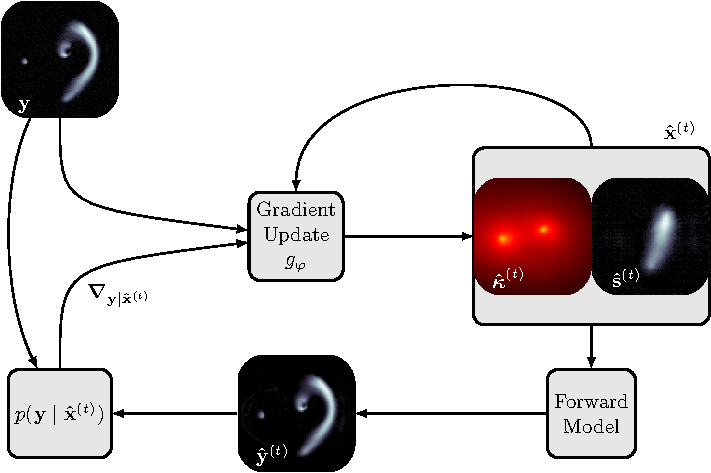
\includegraphics[width=0.7\linewidth]{figures/schematic_rim}
        \caption{Rolled computational graph of the RIM. Dashed arrows represent operations not recorded for BPTT.}
        \label{fig:rolled graph}
\end{figure}


We follow previous works in setting a uniform weight over the time 
steps ($\mathbf{w}^{(t)} = \frac{\mathbf{w}}{T}$). 
The choice of the pixel weights $\mathbf{w}_i$ is informed
by our empirical observations when training the network. Details are reported in appendix \ref{ap:rim training and opt}.

%In figure \ref{fig:unrolled_graph}, we show the unrolled computational graph of the RIM. 
In Figure \ref{fig:rolled graph}, we show the rolled computational graph of the 
RIM. During training of the neural network $g_\varphi$, operations along the solid arrows are being 
recorded for backpropagation through time. 
The recording is stopped along the dashed arrow since these operations 
are part of the forward modelling process and contain no trainable parameters.
%By avoiding the computation of these gradients, training time is reduced and 
%knowledge about the inner workings  
%of a specific likelihood (and forward model) is insulated from the optimization algorithm.
%This is analogous to a common RNN use-case like text generation, where the process responsible 
%for producing the next element in a time series is a black box to the optimization 
%algorithm. 

The gradient of the likelihood is computed using automatic differentiation. Following 
\citep{Modi2021}, we preprocess the gradients using the Adam algorithm \citep{Kingma2014}. 
For clarity, we only illustrate this step in Figure \ref{fig:unet}. 
% \vfill\null

\begin{figure*}[ht!]
        \centering
        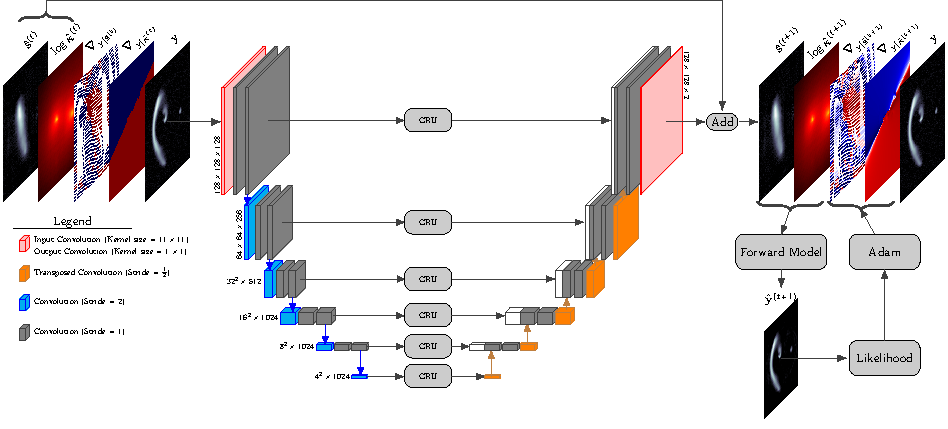
\includegraphics[width=\textwidth]{figures/unet_architecture.pdf}
        \caption{
A single time step of the unrolled computation graph of the RIM.
GRU units are placed in the skip connections to guide the 
reconstruction of the source and convergence. A schematic of the steps to compute 
the likelihood gradients is shown in the bottom right of the figure, including the 
Adam processing step of the likelihood gradient.}
        \label{fig:unet}
\end{figure*}

\subsection{The Neural Network}\label{sec:gradient model}


The neural network architecture is illustrated in Figure \ref{fig:unet}, which shows 
a single time step of the unrolled computation graph of the RIM.
We use a U-net \citep{Ronneberger2015} architecture 
with Gated Recurrent Units \citep[GRU:][]{Cho2014} placed in each skip connection. 

Each GRU cell has its own memory tensor that is updated through time at each iteration of 
equation \ref{eq:RIM}. The shape of a memory tensor is set to match the
feature tensor fed into it from the parent layer in the network graph. 
Instead of learning a compressed representation like in the hourglass
architecture (or autoencoder), the U-net architecture naturally separates the spatial 
frequency components of the signal into its vertical levels. The first level generally encodes 
high frequency features while the lower levels encode low frequency features (due to downsampling of the feature maps). 
Adding an independent memory unit 
at each level preserve this property.

Convolutional layers with a stride of 2 are used for downsampling and 
stride of $\frac{1}{2}$ for upsampling of the feature maps
(identified in blue and orange respectively in figure \ref{fig:unet}). Half-stride convolutions are implemented in practice with the transposed convolution layers from \texttt{Tensorflow} \citep{tensorflow}.
Most layers use a kernel size of $3\times3$, except the first and last layer. 
The first layer has 
larger receptive field ($11\times11$) in order to capture more details in the input tensor. 
The last layer has kernels of size $1\times 1$. 
A $\tanh$ 
activation function is used 
for each convolutional layer, including strided convolutions, except for the output 
layer. The U-net outputs an image tensor with two channels, one dedicated for the update of the source 
and the other for the update of the convergence (see figure \ref{fig:unet}). 
% \vfill\null
%\columnbreak


% Talk about this choice
% Shared memory is important, possibly more than the notion that source and kappa require very different 
% reconstruction procedure (because of different structure etc).

% Choice of model correspond to choosing an inductive bias, or how the function should behave 
% for points in and out of the dataset
% Generalization means the ability to make prediction about the behavior of the function 
% at novel points in the domain of the function.
% In the meta-learning framework, examples are problem instances. Generalization means to transfer 
% knowledge accross problem instances.
% The reuse of the problem structure is known as transfer learning. In the context of meta-learning, 
% this is cast as generalization.


\subsection{Fine-Tuning}\label{sec:fine-tuning}

\subsubsection{Objective function}
Once trained, the RIM produces a baseline (point)
estimate of the parameters $\mathbf{x}$ given a noisy observation $\mathbf{y}$, a PSF and a noise covariance matrix. 
%We note $(\mathbf{y},\Pi,C) \sim \mathcal{T}$.
We now concern ourselves with a strategy to improve 
this estimate. 
This is important 
for observations with high SNR, for which the estimate
must be very accurate to model all the fine features present in the arcs.
The metric for the goodness of fit 
is the reduced chi squared $\chi^2_\nu = \frac{\chi^2}{\nu}$, 
where $\nu$ is the total number of degrees of freedom which here corresponds to 
the total number of pixels in $\mathbf{y}$.
Generally, our goal will be to reach $\chi^2_\nu = 1$, or equivalently $|\chi^2 - \nu| = 0$, 
which suggests that the RIM's estimate has modeled all the signal 
to be recovered from the observations. 
We note that such a problem is exceedingly  
difficult at high SNR. 

We note that we can optimize the log-likelihood directly w.r.t.\ the network weights given an appropriate prior on those weights (to avoid forgetting the implicit priors that have been learned during training, see section \ref{sec:transferlearning}). The new objective function is given by
\begin{equation}\label{eq:MAP} 
        \hat{\varphi}_{\mathrm{MAP}} = \underset{\varphi}{\mathrm{argmax}}\,\, 
        \frac{1}{T}\sum_{t=1}^{T} \log p(\mathbf{y} \mid \mathbf{\hat{x}}^{(t)}) + \log p(\varphi) \, ,
\end{equation} 
where $\varphi$ are the network weights, $\log p(\mathbf{y} \mid \mathbf{\hat{x}}^{(t)})$ is the log-likelihood, and $\log p(\varphi) $ is the log prior over the network weights.
Unlike the loss in equation \eqref{eq:Loss}, this objective function makes no use of labels 
($\mathbf{x}$). 
This allows us to use equation \eqref{eq:MAP} at test time in order to fine-tune the RIM's weights to a specific test example. 

\subsubsection{Transfer Learning}
\label{sec:transferlearning}
We now address the issue of transferring knowledge from the training task defined by the loss function in equation \eqref{eq:Cost}, 
to a test task specific to an observation,  as defined by the loss given in equation \eqref{eq:MAP}.
The reader might refer to reviews on transfer learning \citep{Pan2010,Zhuang2019} 
for a broad overview of the field. The strategy we outline falls within 
the category of inductive transfer learning.

%Despite the second term in Eq \eqref{eq:MAP}, we find 

% Since the data likelihood $p(\mathbf{y} \mid \mathbf{x})$ 
% does not contain \textit{a priori} information 
% about the solution $\hat{\varphi}_{\mathrm{MAP}}$,
% inductive biases must be introduced to make 
% the problem \eqref{eq:MAP} well-posed. Thus, we
% \begin{enumerate}[label=(\subscript{\mathcal{H}}{{\arabic*}})]
%         %\setcounter{enumi}{3}
%         \item \label{prior:initialization} initialize the network parameters with $\varphi_{\mathcal{D}}^{\star}$; 
%         \item \label{prior:early stopping} apply early stopping when a maximum number of steps is reached or 
%                 $\chi^2_\nu \leq 1$;
%         % \item \label{prior:learning rate} use a small learning rate.
% \end{enumerate}
% \ref{prior:early stopping} and \ref{prior:learning rate} encode the assumption 
% that the optimal estimator is to be found \textit{near} the initialization.

\begin{figure}[tb!]
       \centering 
       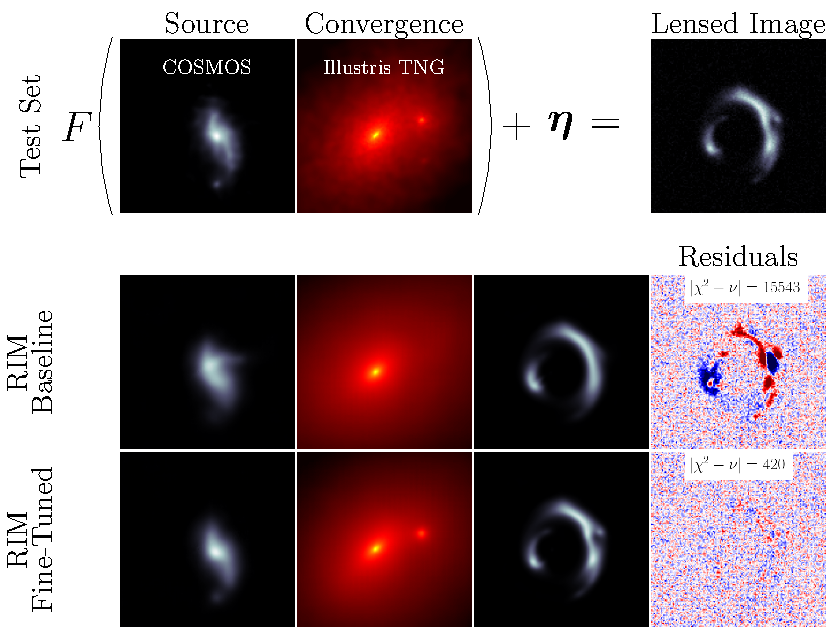
\includegraphics[width=0.8\linewidth]{figures/main_figurev2}
       \caption{Example of a simulated lensed image in the test set that 
exhibits a large deflection in its eastern arc which indicates the presence of a massive object
 --- in this case a dark matter subhalo. The fine-tuning procedure is able to recover 
this subhalo because of its strong signal in the lensed image and reduces the residuals 
to noise level.}
       \label{fig:main figure}
\end{figure}

Optimizing the log-likelihood alone without a prior term over the weights (i.e.~just the first term from the r.h.s.~in \eqref{eq:MAP}) by initializing the weights at $\varphi^\star_\mathcal{D}$ is not strong 
enough to preserve the knowledge learned from the training task. 
This has long been observed in the literature and was coined as the 
catastrophic interference phenomenon in 
connectionist networks \citep{McCloskey1989,Ratcliff1990}.
In summary, a sequential learning problem exhibits catastrophic 
forgetting of old knowledge when confronted with new examples (possibly 
from a different distribution or process), in a manner 
\begin{enumerate}%[label=(\subscript{\mathrm{CF}}{{\arabic*}})]
        \item \label{cf:steps} proportional to the amount of learning;
        \item \label{cf:weights} strongly dependant to the disruption of the parameters
                involved in representing the old knowledge.
\end{enumerate}
While introducing an early stopping condition could 
potentially alleviate the former issue, the latter could still remain a problem.

We therefore follow the work of \citet{Kirkpatrick2016} to define a prior distribution
over $\varphi$ that address this issue
\begin{equation}\label{eq:Prior} 
        \log p(\varphi) \propto -\frac{\lambda}{2}\sum_{j} \mathrm{diag}(\mathcal{I}(\varphi_{\mathcal{D}}^{\star}))_{j} 
        (\varphi_j - [\varphi^{\star}_{\mathcal{D}}]_{j})^{2}\, .
\end{equation} 
where $\mathrm{diag}(\mathcal{I}(\varphi_{\mathcal{D}}^{\star}))$ is the diagonal of the 
Fisher information matrix 
encoding the amount of information that  
some set of gravitational lensing systems from 
the training set, and similar to the observed 
test task, carries about the baseline RIM weights $\varphi_{\mathcal{D}}^{\star}$ 
--- the parameters that minimize the empirical risk (equation \ref{eq:Cost}).
We can also understand this prior using the
Cramér-Rao lower bound 
\citep{Rao1945,Cramer1946}.
%\begin{equation}\label{eq:iCramerRao}
        %\mathrm{Var(\varphi)} \geq \underbrace{(1 + \mathrm{Bias}_{\mathcal{D}}(\varphi))^{2}}_{\lambda_b}\mathcal{I}(\varphi)^{-1}.
%\end{equation} 
The prior can thus be framed as a multivariate 
Gaussian distribution characterised by a diagonal covariance matrix with $\mathrm{diag}(\mathcal{I})$ as its inverse 
and by $\varphi^{\star}_{\mathcal{D}}$ as its first moment. 
Within this view, the  
Lagrange multiplier is 
tuning our estimated uncertainty about the neural network weights 
for the particular task at hand.  
We have included a derivation 
of this term in the appendix \ref{ap:ewc}.

%We define the distribution of examples from $\mathcal{D}$ similar to the test task $\mathcal{T}$ with 
%the surrogate conditional $\tilde{p}(\mathcal{D} \mid \mathcal{T})$. 
Examples are drawn from the set of training examples similar to the test task by sampling the latent space of two variational autoencoders (VAE) that model a distribution over the background sources and the convergence maps respectively (as described in Section \ref{sec:source} and \ref{sec:kappa}) near the baseline prediction of the RIM. In practice, we choose an isotropic Gaussian distribution centered around $\hat{\mathbf{z}}^{(T)}$ --- 
the latent code of the baseline prediction --- as a sampling distribution. While we leave the possibility of improving this choice to future work, it is sufficient for our goals. 
Figure \ref{fig:vae fine-tuning} illustrates examples of what is meant here by \textit{similar}. 

\begin{figure}[t!]
        \centering
        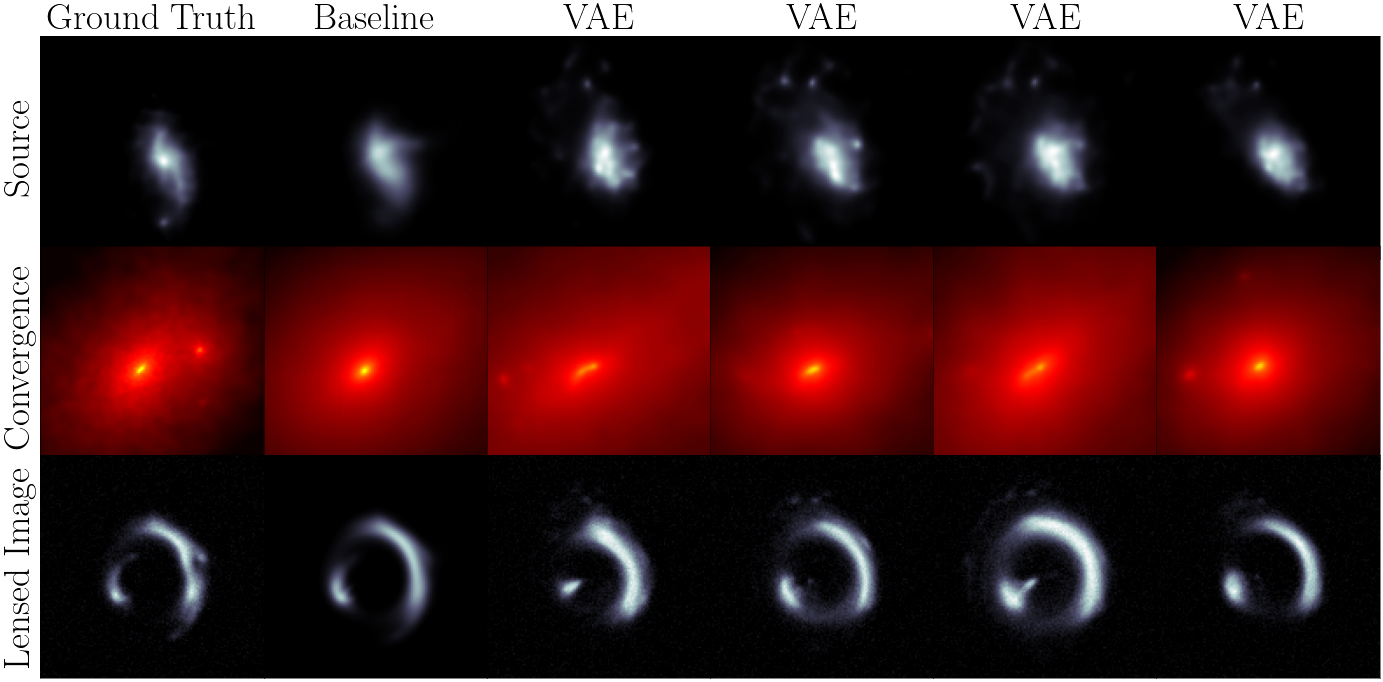
\includegraphics[width=0.8\linewidth]{figures/vae_samples_similar_to_highlight}
        \caption{Examples similar to the test task, also shown in Figure \ref{fig:main figure}. The first column shows the ground truth used to simulate the lensed image. The second column shows the baseline prediction that is then encoded in the latent space of the VAE in order to sample the next 4 columns.
}
        \label{fig:vae fine-tuning}
\end{figure}

%By definition, the Fisher matrix is the 
%expected value of the observed information that 
%the examples carry about $\varphi$. 

%We can, however, make use of theoretical and 
%experimental evidence that overparametrized 
%neural networks exhibits a spectral bias \citep{Rahman2018} 
%toward learning low frequencies first during training. We observe 
%that the baseline model generally 
%provides a coherent prediction ($\gamma(k) = 1$) in the low frequency 
%regime, which is consistent with a spectral bias hypothesis. 
%This suggest a possible approach to ground our method. 
%The MLE-optimal estimator should at least 
%preserve the low frequency features predicted by the baseline. 
%Otherwise, we might suspect that the optimisation procedure 
%has found a degenerate solution that is not consistent with the 
%prior learned by the baseline.

%This also points to interesting strategies that could alleviate 
%overfitting. For instance, freezing the deeper layers of the U-net during 
%fine-tuning might preserve the low frequency features learned during pretraining. 
%This is also suggested as a strong regularization method in \citet{Li2018}. 
%We explore such ideas in the appendice


\section{Data}\label{sec:data}

\subsection{COSMOS}\label{sec:source}
The maps of surface brightness of background sources are taken from the \textit{Hubble Space Telescope} (\textit{HST}) 
Advanced Camera for Surveys Wide Field Channel COSMOS field \citep{Koekemoer2007,Scoville2007},
a $1.64\,\mathrm{deg}^{2}$ contiguous survey acquired in the F814W filter. 
A dataset of magnitude limited ($\mathrm{F814W} < 23.5$) deblended galaxy postage stamps \citep{Leauthaud2007} was compiled as 
part of the GREAT3 challenge \citep{Mandelbaum2014}. The data is 
publicly available \citep{Mandelbaum2012}, and the preprocessing is done through the open-source software 
\texttt{GALSIM} \citep{Rowe2015}. \par

We apply the 
\texttt{marginal} selection criteria (see the \texttt{COSMOSCatalog} class) and impose a flux per image
greater than $50\,\,\mathrm{photons}\,\,\mathrm{cm}^{-2}\,\mathrm{s}^{-1}$. 
This final set has a total of 13\,321 individual images.
Each image is saved as a postage stamp of $158^2$ pixels. 
We then subtract the background from each image, apply a random shift, rotate them by an angle multiple of $90^\circ$, crop them down to $128^{2}$ pixels, and finally normalize them to pixel intensities in the range $[0,1]$. We then train an autoencoder to denoise the galaxy images \citep{Vincent2008,Vincent2010}. More specifically, we use the informational bottleneck principle \citep{Tishby2000} to learn a lossy lower-dimensional representation of the data. For a generic CNN autoencoder, this amount to learning a low-pass frequency filter on the COSMOS dataset. Indeed, CNNs are known to exhibit a spectral bias in their learning phase \citep{Rahaman2018}, which we exploit to our advantage in order to filter pixel noise from the galaxy surface brightness. Furthermore, using an expressive CNN autoencoder produces much less artifacts than a naive implementation of such a low-pass filter --- e.g.\ by masking Fourier modes. 

We split the galaxies into a training set (90\%) and a test set (10\%). 
The augmented training set (${\sim50\,000}$ images) is then used to train a VAE, as described in Section \ref{sec:vae training}, and produce simulated observations to train the RIM.

\begin{figure}[t!]
        \centering
        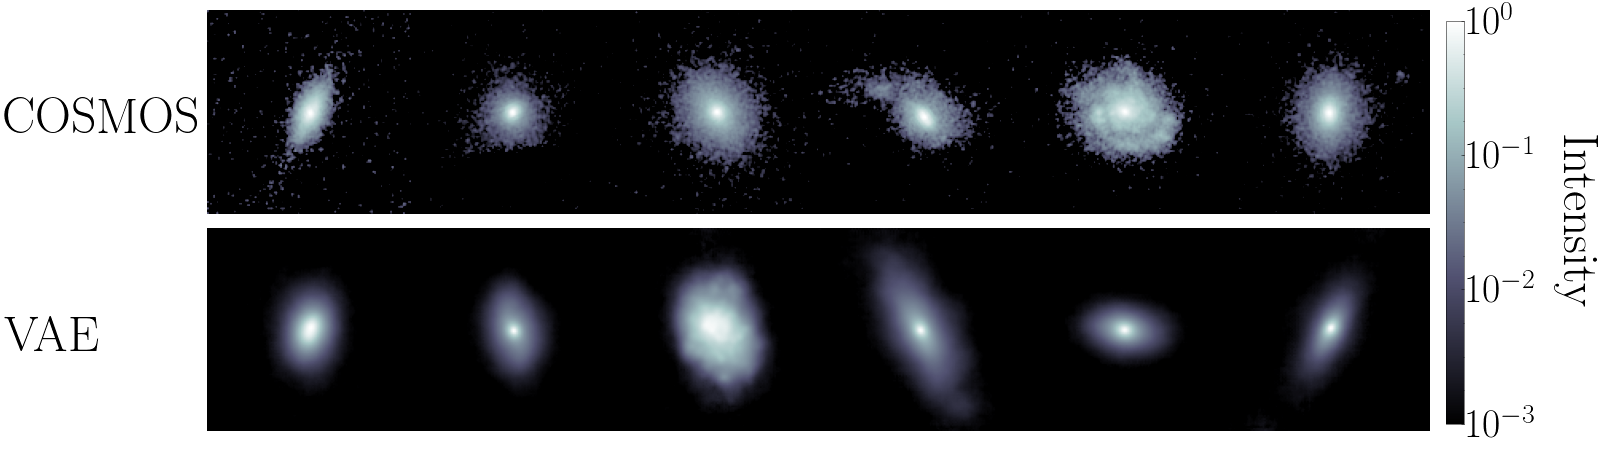
\includegraphics[width=0.8\linewidth]{figures/gal_vae_sample}
        \caption{Examples of COSMOS galaxy images 
                (top row) and VAE generated samples (bottom row) used as labels in $\mathcal{D}$.}
        \label{fig:source}
\end{figure}


\subsection{IllustrisTNG}\label{sec:kappa}
\subsubsection{Smooth Particle Lensing}\label{sec:SPL}
To compute convergence maps from an N-body simulation, 
we use Kernel Density Estimation to produce smooth densities on a regular grid from discrete simulation particles.
This reduces the particle noise affecting all 
important lensing quantities. At the same time, the choice of the kernel size 
is important to preserve substructures in the 
lens that we might potentially be interested in. Following \citet{Aubert2007,Rau2013}, we use Gaussian smoothing with an adaptive kernel size determined by the distance of the 64\textsuperscript{th} nearest neighbours of 
a given particle $D_{64,i}$. 
\begin{equation}\label{eq:Ksmooth}
\begin{aligned}
    \kappa(\mathbf{x}) &= \frac{1}{\Sigma_{\mathrm{crit}}} \sum_{i=1}^{N_{\mathrm{part}}}
        \frac{m_i}{2 \pi \hat{\ell}^2_i} 
        \exp \left(-\frac{1}{2} \frac{(\mathbf{x} - \mathbf{x}_i)^2}{\hat{\ell}_i^2}  \right) \\
    \hat{\ell}_i &= \sqrt{\frac{103}{1024}}D_{64,i}.
\end{aligned}
\end{equation}
The nearest neighbours are found by fitting a k-d tree ---  implemented in 
\texttt{scikit-learn} \citep{scikit-learn} --- 
to the $N_{\mathrm{part}}$  particles 
in a cylinder centered on the centre of mass of the halo of interest.
The critical surface density is defined as
\begin{equation}\label{eq:Scrit}
\Sigma_{\mathrm{crit}} = \frac{4 \pi G}{c^ 2} \frac{D_\ell D_{\ell s}}{D_s},
\end{equation}
where $D_\ell$, $D_s$ and $D_{\ell s}$ are angular diameter distances to the lens, source and between the lens and the source respectively, 
$G$ is the gravitational constant, and $c$ the speed of light.

\subsubsection{Preprocessing}
The projected surface density maps (convergence) of lensing galaxies 
were made using the redshift $z=0$ snapshot  
of the IllustrisTNG-100 simulation \citep{Nelson2018} 
in order to produce physically realistic realizations of density maps containing dark and baryonic matter.
We selected 1604 halos with the criteria that they have a total
dark matter mass of at least $9\times10^{11} M_{\odot}$. We then collected all 
dark matter, gas, stars and black holes particles from the data in the vicinity of the halo. We then create a smooth projected surface density map as prescribed in section \ref{sec:SPL}.

\begin{figure}[t!]
        \centering
        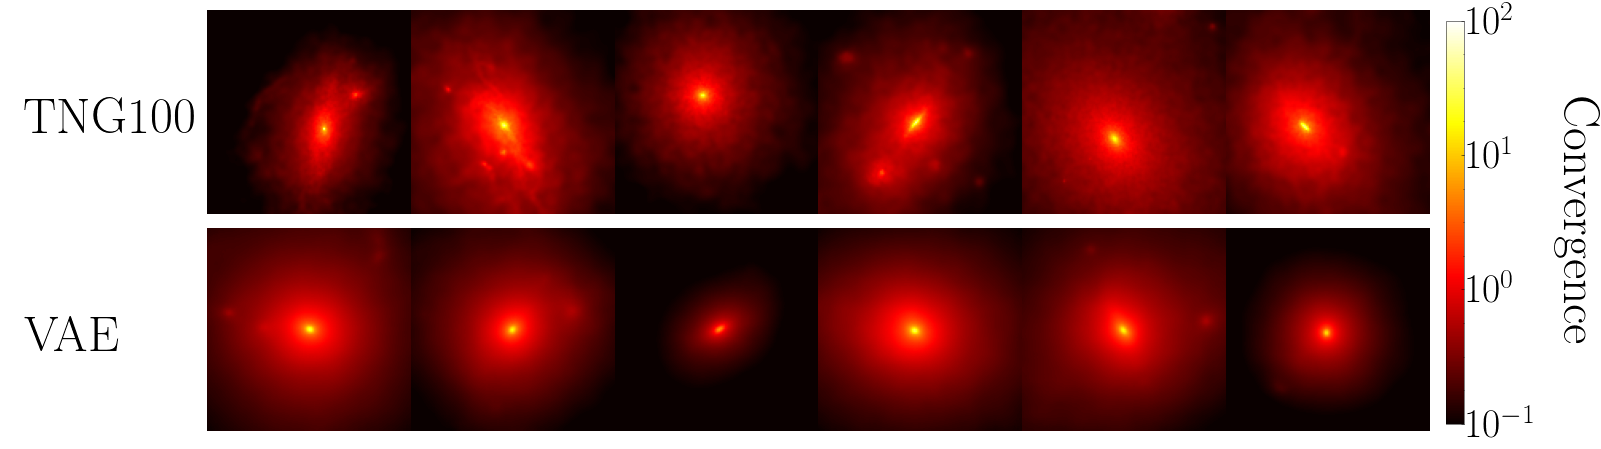
\includegraphics[width=0.8\linewidth]{figures/kap_vae_sample}
        \caption{Examples of smoothed Illustris TNG100 convergence map (top row) 
        and VAE generated samples (bottom row) used as labels in $\mathcal{D}$.}
        \label{fig:kappa}
\end{figure}

We adopt the $\Lambda$CDM cosmology from 
\citet{PlanckCollaboration2018} with $h=0.68$ to compute 
angular diameter distances. We also fix the 
source redshift to $z_s=1.5$ and the deflector redshift to $z_\ell=0.5$. 
We note that changing the redshifts or the cosmology 
only amount in a rescaling of the $\kappa$ map by a global scalar. Thus, this choice does not change the generality of our method.
The smoothed density maps from equation \eqref{eq:Ksmooth} are 
rendered into a regular grid of $188^2$ pixels with a comoving field of view of $105\,\,\mathrm{kpc}/h$. 
To avoid edge effects in the pixelated maps, 
we include particles outside of the field of view in the sum of equation \eqref{eq:Ksmooth}.
\par
Before applying augmentation or considering different projections, our dataset of halos is split into a 
training set (90\%) and a test set (10\%), in order to make sure that the test set consists only 
of convergence maps unseen by the RIM during training.
We take 3 different projections ($xy$, $xz$ and $yz$) of each 3D particle 
distribution, which amounts to a dataset with a total of $4\,812$ individual convergence maps. 
Random rotations by an angle multiple of $90^{\circ}$ and random shifts to the pixel coordinates 
are applied to each image. The $\kappa$ maps are then rescaled by a random factor to change their 
estimated Einstein radius to the range 
$[0.5,\,2.5]$ arcseconds.
The Einstein radius is defined as
\begin{equation}\label{eq:ThetaE}
        \theta_E = \sqrt{\frac{4GM(\theta_E)}{c^ 2} \frac{D_{\ell s}}{D_\ell D_s}}
\end{equation} 
where $M(\theta_E)$ is the mass enclosed inside the Einstein radius. In practice, we estimate this quantity 
by summing over the mass of pixels with a value greater than the critical density ($\kappa > 1$). 
For data augmentation purposes, this procedure gives a good enough estimate of the lensed image separation resulting from a given $\kappa$ map. 
We test multiple scaling factors for each $\kappa$ map, then uniformly sample between those that produce an estimated 
Einstein radius within the 
desired range. This step is used to remove any bias in the Einstein radius that might come from the mass function 
of the simulation.

The final maps are cropped down to $128^2$ pixels.
Placed at a redshift $z_\ell=0.5$, a $\kappa$ map will thus span an angular field of view of $7.69''$ with 
a resolution similar to \textit{HST}. 
%This field of view is wide enough to cover a typical gravitational 
%lens observed in the sky, which partly justify our choice for the comoving field of view earlier. 
With these augmentation procedures, a total of $50\,000$ maps are created from the training split
to train a VAE, as described in Section \ref{sec:vae training}, and produce simulated observations to train the RIM. 

\subsection{Simulated Observations}\label{sec:simulated observation}
Having defined a source map and a convergence map, we apply the ray tracing simulation 
described in section \ref{sec:forward model} to produce a lensed image. 

For each lensed image, a Gaussian PSF is 
created with a full width at half maximum (FWHM) 
randomly generated from a truncated normal distribution.
The support of the distribution is truncated below by the 
angular size of a single pixel and above by the angular size of 4 pixels. 
White noise with a standard deviation randomly generated from a truncated normal distribution 
is then added to the convolved lensed image to simulate noisy observations. These noise realizations result in SNRs between 
$10$ and $1000$. For simplicity, we define $\mathrm{SNR} = \frac{1}{\sigma}$. 
This definition is equivalent to the peak signal-to-noise ratio. 

%We set the observed image field of view to match with the convergence field view ($7.69''$). 
%We choose the background field of view to be $3''$.
To ensure that the images are representative of strongly lensed source, we require a minimum flux magnification of 3. We
also make sure that most pixel coordinates in the image plane are mapped inside the 
source coordinate system through the lens equation \eqref{eq:LensEquation}. 

\begin{table}[htb!]
\centering
\caption{Physical model parameters.}
\label{tab:phys}
\begin{tabular}{ccc}
        Parameter &  Distribution/Value \\
        \hline \hline
        Lens redshift $z_\ell$ & $0.5$ \\
        Source redshift $z_s$ & $1.5$ \\
        Field of view ('') & $7.69$ \\
        Source field of view ('') & $3$ \\
        PSF FWHM ('') & $\mathcal{TN}(0.06,\, 0.3;\, 0.08,\, 0.05)$
        \footnote{We defined the parameters of the truncated normal in the order $\mathcal{TN}(a,\, b;\, \mu,\, \sigma)$, where $[a,\, b]$ defines the support of the distribution.} \\
        Noise amplitude $\sigma$ & $\mathcal{TN}(0.001,\, 0.1;\, 0.01,\,0.03)$\\
        \hline
\end{tabular}
\end{table}

In total, $400\,000$ training observations are simulated from random pairs of COSMOS sources 
and IllustrisTNG convergence maps in order to train the RIM. 
An additional $200\,000$ observations are created from pairs 
of COSMOS sources and pixelated SIE convergence maps. 
The parameters for these $\kappa$ maps are listed in table \ref{tab:sie}. 
% We expect some lensing configurations like doubly imaged systems to poorly constrain the inner structure of the 
% mass distribution. 
% Building an inference pipeline with strong constraints (other than the lensed image) on the 
% slope of the profile goes beyond the scope of this work. 
% As such, imposing an implicit prior for the slope through 
% the dataset is sufficient for our goal. 
% It is also motivated by the \textit{bulge-halo conspiracy} --- 
% the observation that most lensing configurations observed in the sky can be explained 
% to a first order approximation by 
% an average slope consistent with an isothermal profile \citep{Auger2010,Dutton2014}.

\begin{table}[htb!]
\centering
\caption{SIE parameters.}
\label{tab:sie}
\begin{tabular}{ccc}
        Parameter &  Distribution \\
        \hline \hline
         Radial shift ('') & $\mathcal{U}(0, 0.1)$ \\
        Azimutal shift & $\mathcal{U}(0, 2\pi)$ \\
        Orientation & $\mathcal{U}(0, \pi)$ \\
        $\theta_E$ ('') & $\mathcal{U}(0.5, 2.5)$ \\
        Ellipticity & $\mathcal{U}(0, 0.6)$ \\
        \hline
\end{tabular}
\end{table}


We generate $1\,600\,000$ simulated observations from the VAE 
background sources and convergence maps as part of the training set. We apply some validation checks to each example in order to avoid configurations like a single image of the background source or an Einstein ring cropped by the field of view.
% In principle, we could generate as many simulated observations as needed from the VAE. 
% However, having a set of finite, fixed size lets us apply some validation checks to each 
% example in order to avoid configurations like a
% single image of the background 
% source or an Einstein ring cropped by the field of view.




\section{Training}\label{sec:training}

\subsection{VAE}\label{sec:vae training}
Here, we describe the training of two VAEs that are used to produce density maps and images of unlensed background galaxies to train and test our inference model. For an introduction to VAEs we refer the reader to \citet{Kingma2019}.

As mentioned in \citet{Kingma2019}, direct optimisation 
of the ELBO loss can prove difficult because the reconstruction term $\log p_\theta (\mathbf{x} \mid \mathbf{z})$ 
is relatively weak compared to the Kullback Leibler (KL) divergence term. To alleviate this issue, 
we follow the work of \citet{Bowman2015} and \citet{Sonderby2016} in setting a warm-up 
schedule for the KL term, starting from $\beta=0.1$ up to $\beta_{\mathrm{max}}$. 

Usually, 
$\beta_{\mathrm{max}} = 1$ is considered optimal since it matches the original ELBO  
objective derived by \citet{Kingma2013}. 
However, we are more interested in the 
sharpness of our samples and accurate inference around small regions of the latent 
space for fine-tuning. Thus, setting $\beta_{\mathrm{max}} < 1$ allows us to increase 
the size of the information bottleneck (i.e.~latent space) of the VAE 
and improve the reconstruction cost of the model. 
This is a variant of the $\beta$-VAE \citep{Higgins2017}, where $\beta > 1$ was found 
to improve disentangling of the latent space \citep{Burgess2018}. 

The value for $\beta_\mathrm{max}$ and the steepness of the schedule 
are grid searched alongside the architecture for the VAE. 
These values are found in practice by 
manually looking at the quality of generated samples for different VAE 
hyperparameters. A similar method is explored and formalized in the 
InfoVAE framework \citep{Zhao2017}.


A notable element of the VAE architecture is the use of a fully connected
layer to reshape the features of the convolutional layer into the chosen 
latent space dimension. Following the work of \citet{Lanusse2021}, we introduce 
an $\ell_{2}$ penalty between the input and output of the bottleneck 
dense layers to encourage an identity mapping. This regularisation 
term is slowly removed during training.


\subsection{RIM}\label{sec:rimtraining}

The architecture of the neural network was grid searched on 
a smaller dataset ($\lesssim 10\,000$ examples) 
in order to quickly identify a small set
of valid hyperparameters. Then, the best hyperparameters were 
identified using a two-stage training process on the training dataset. 
In the first stage, we trained 24 different architectures from this small hyperparameter set for approximately 4 days (wall time using a single Nvidia A100 GPU). 
Different architectures would have a training time much longer than others, and this 
was factored in the architecture selection process. For example, adding more time steps ($T$) to the recurrent relation \eqref{eq:RIM} 
would yield better generalisation on the test set, but this 
would come at great costs to training time until convergence. 

Following this first stage, 4 architectures were deemed efficient enough 
to be trained for an additional 6 days. 
We only report the results for the best architectures out of these 4.
%We report the hyperparameters for 
%the best architecture after this second stage of training in table \ref{tab:baseline hparams}.

Each reconstruction is performed by fine-tuning the baseline model 
on a test task composed of an observation vector, a PSF, and a noise covariance.
In practice, fine-tuning predictions on the test set of $3\,000$ examples can be accomplished in parallel so as to be done in at most a few days by spreading the computation on $\sim 10$ Nvidia A100 GPUs. Each reconstruction uses at most 2000 steps, correspondling to approximately $20$ minutes (wall-time) per reconstruction. Early stopping is applied when the $\chi^2$ reaches noise level. The hyperparameters for this procedure are reported in Table \ref{tab:fine-tuning hparams}.


\begin{table}[H]
        \centering
        \caption{Hyperparameters for fine-tuning the RIM.}
        \label{tab:fine-tuning hparams}
        \begin{tabular}{cc}
                Parameter & Value \\\hline\hline
                Optimizer & RMSProp \\
                Learning rate & $10^{-6}$\\
                Maximum number of steps & $2\,000$\\
                $\lambda$ & $2\times 10^{5}$\\
                $\ell_2$ & 0 \\
                Number of samples from VAE & 200 \\
                Latent space distribution & $\mathcal{N}(\mathbf{z}^{(T)}, \sigma=0.3)$
                \footnote{$\mathbf{z}^{(T)}$ is the latent code of the RIM baseline source or convergence.}\\
                \hline
        \end{tabular}
\end{table}



\begin{figure}[H]
        \centering
        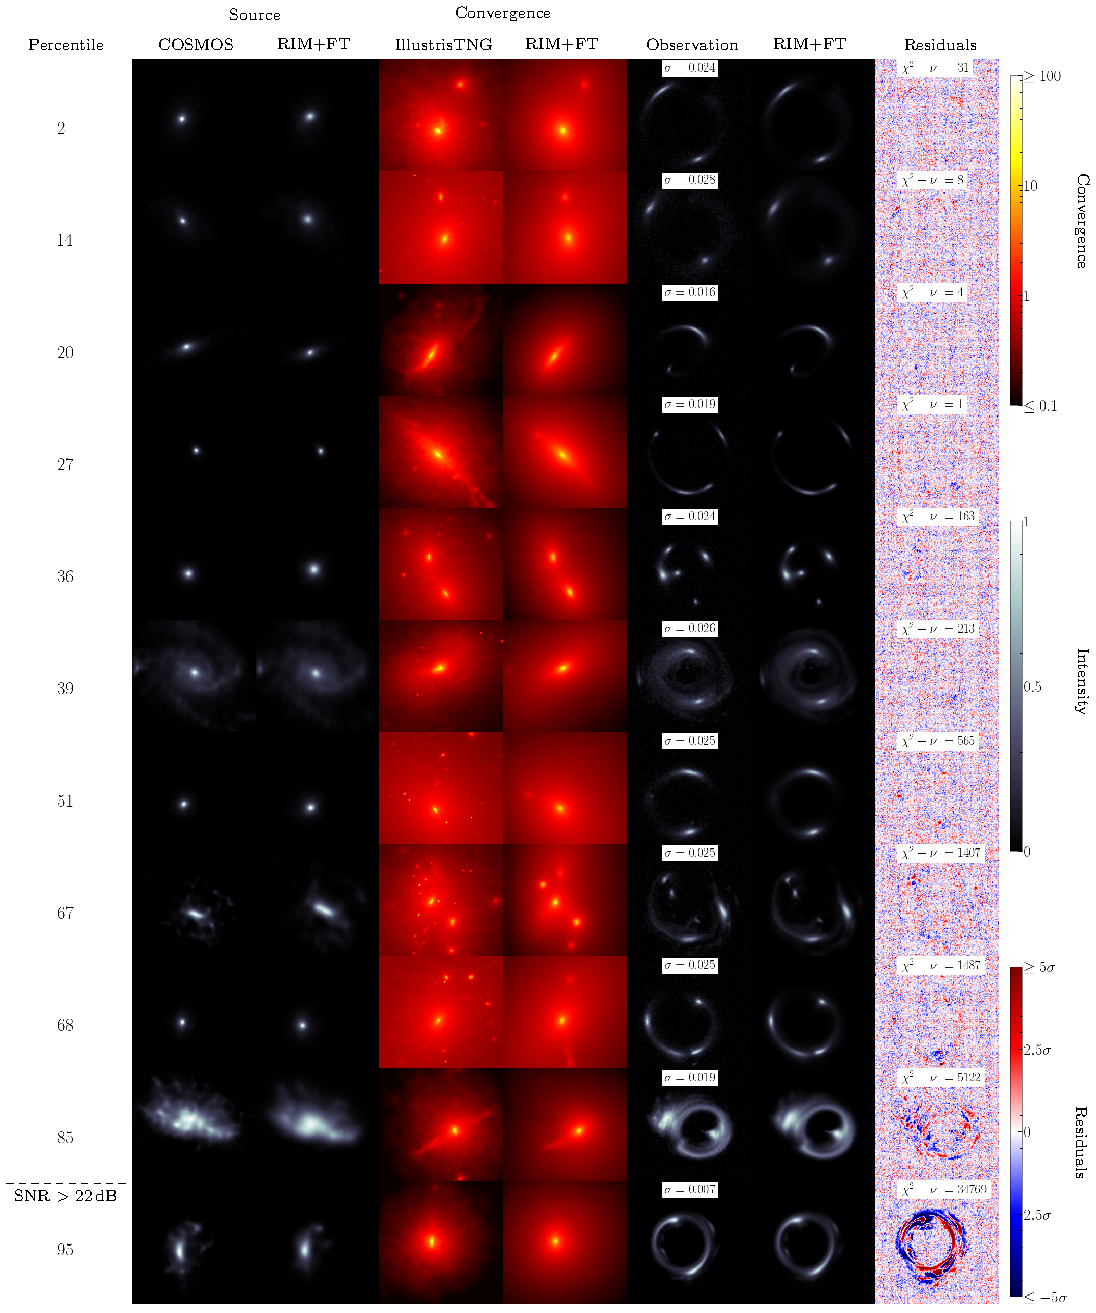
\includegraphics[width=\linewidth]{figures/main_result}
        \caption{
                Sample of the fine-tuned RIM reconstructions 
                on a test set of 3000 examples. 
                Examples are ordered from the best $\chi^2$ (top) to the worst (bottom). 
                The percentile rank of each example is in the leftmost column. 
                The last example 
        shown has SNR above the threshold defined in Figure \ref{fig:chi squared vs noise}.}
        \label{fig:main result}
        %\vspace{-1.5pt} % fix
\end{figure}

\begin{figure}[H]
        \centering
        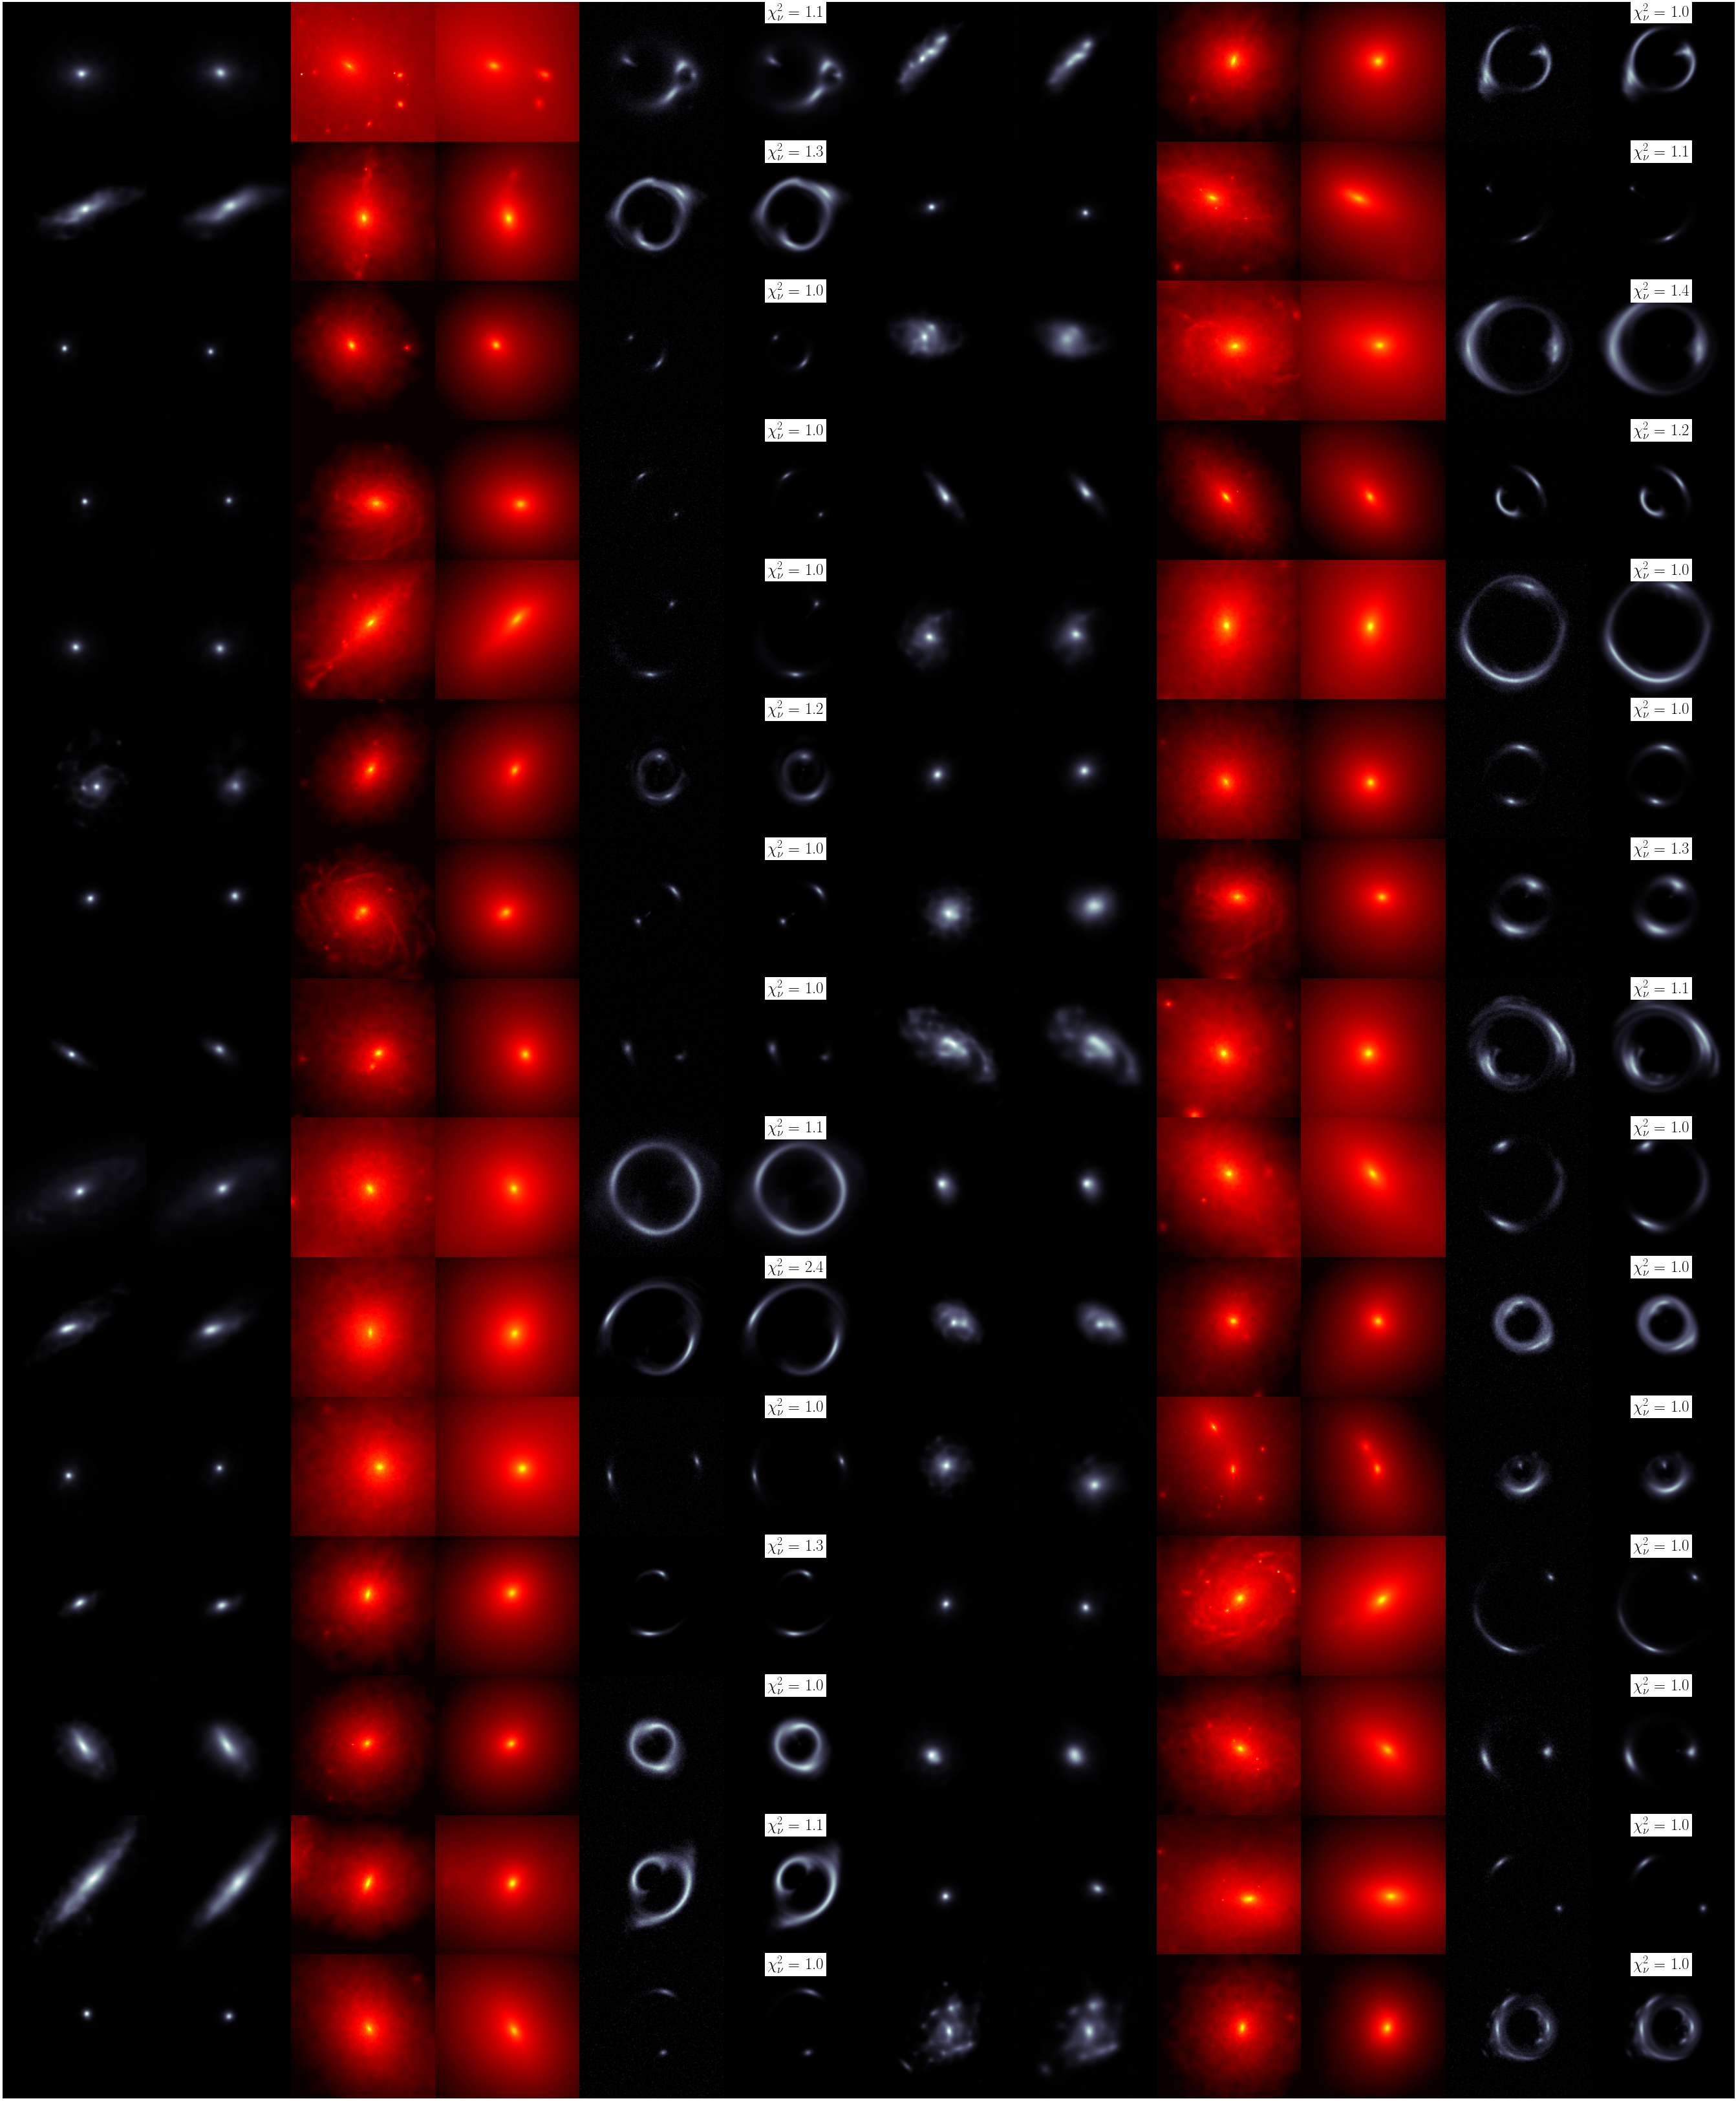
\includegraphics[width=\linewidth]{figures/test_set_no_cherry_pick}
        \caption{
                30 reconstructions taken at random from the test set of 3000 examples simulated from COSMOS 
                and IllustrisTNG data at high SNR.
                The colorscale are the same as in Figure \ref{fig:main result}.}
        \label{fig:random sample}
	\vspace{-1.5pt} % fix
\end{figure}


\section{Results}\label{sec:results}

In this section, we present the performance of our model 
on the held out test set. A sample of 3000 reconstruction 
problems is generated from the held-out \textit{HST} and IllustrisTNG data 
with noise levels and PSFs similar to the training set.

\subsection{Goodness of Fit}
Figure \ref{fig:main result} shows a sample of reconstructions for high SNR data with a wide range of lensing configurations from the test set.
We select examples representative of all levels of reconstruction performance (covering the entire range of goodness of fit) for data with  complex structures in their convergence map to showcase the expressivity of the approach. 
We also show a randomly selected sample from the test set in Figure \ref{fig:random sample}.

\begin{table}[H]
    \centering
    \caption{$\log_{10}$-normal moments of the loss on the test set}
    \label{tab:loss}
    \begin{tabular}{ccc}
        \hline
          Model  & $\mu(\log \mathcal{L}_\varphi)$ & $\sigma(\log \mathcal{L}_\varphi)$ \\
        \hline \hline
        Baseline ($\varphi_{\mathcal{D}}^\star)$ &  -1.96 & 0.36 \\
        Fine-tuned ($\hat{\varphi}_{\mathrm{MAP}}$) & -2.02 & 0.37 \\\hline
    \end{tabular}
\end{table}


\begin{figure}[H]
        \centering
        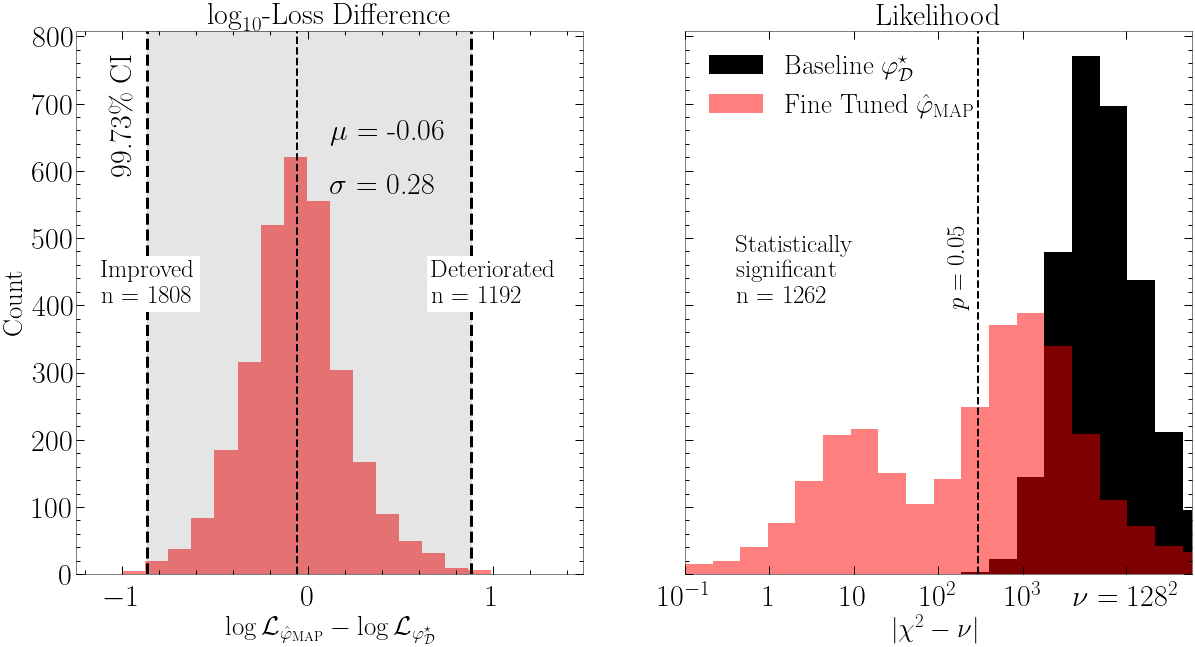
\includegraphics[width=0.8\textwidth]{figures/loss_and_likelihood}
        \caption{Distribution of the goodness of fit for the baseline and fine-tuned network (right panel), as well as log-loss difference between the two network for a given example in the test set (left panel).
}
        \label{fig:loss and chi squared}
\end{figure}


Figure \ref{fig:loss and chi squared} shows a comparison between 
the goodness of fit of the baseline model and the fine-tuned prediction. 
Since we empirically observe that the distribution of the loss on the test set (and the training set) follows a log-normal distribution, we find that it is more informative to look at the $\log$-loss 
distribution to extract information about the fine-tuning procedure. 
The left panel of Figure \ref{fig:loss and chi squared} 
shows the distribution of the log-loss difference between the fine-tuned prediction and the baseline model. This distribution shows that the fine-tuning procedure loss is constrained within $\sim 1$ order of magnitude of the original loss with a probability $>99.73\,\%$. We find that the log-loss difference has a scatter of $\sigma = 0.28$, which is smaller than the scatter of the baseline log-loss over the entire test set $\sigma(\log \mathcal{L}_{\varphi^\star_{\mathcal{D}}}) = 0.36$ reported in Table \ref{tab:loss}.
We note that the loss is not optimized during fine-tuning, still we notice that the fine-tuning procedure does not significantly deteriorate or improve the loss of the baseline prediction on average. We report the first 2 moments of the loss log-normal distribution for the baseline and the fine-tuned reconstructions in Table \ref{tab:loss} in order to explicitly compare them. As can be seen in this table, there is no significant difference between the two distributions. This statement can be proven for the measured mean values --- $\mu(\log \mathcal{L}_{\hat{\varphi}_{\mathrm{MAP}}}) = \mu(\log \mathcal{L}_{\varphi^{\star}_{\mathcal{D}}}) $ --- using the two-sided normal p-value test \citep{Casella2001}, which we find satisfy the null hypothesis with $p=0.87288$ ($Z = -0.16$). All those observations support our claim that EWC regularisation preserves the prior learned during pretraining, or at least that it preserves the surrogate measures of the prior we reported. 

\begin{figure}[H]
        \centering
        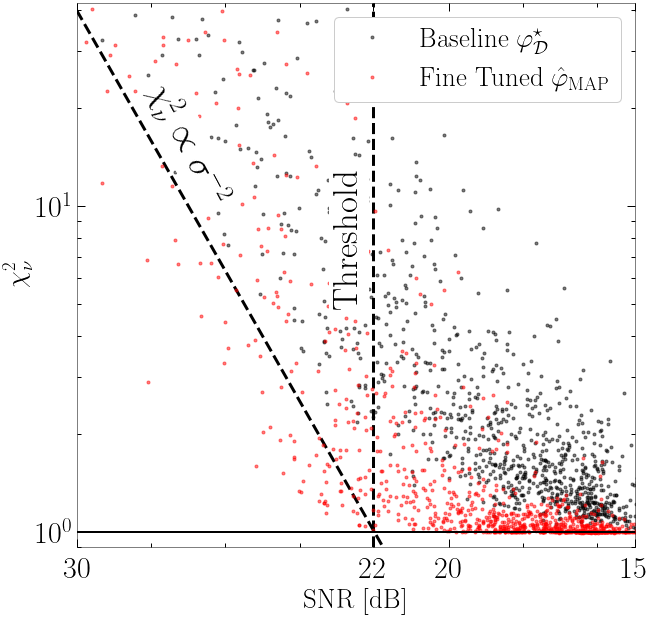
\includegraphics[width=0.6\linewidth]{figures/chisq_vs_noise_ewc}
        \caption{Goodness of fit as a function of SNR shows a threshold 
        behavior where our method reaches its limit.}
        \label{fig:chi squared vs noise}
\end{figure}



The right panel of Figure \ref{fig:loss and chi squared} shows the distribution of  $\chi^2$ for the test set before and after the fine-tuning procedure and the theoretical $\chi^2$ distribution corresponding to $\nu=128^2$ degrees of freedom.
We observe that the fine-tuning procedure significantly improves our $\chi2$, bringing their distribution closer to that of the expected $\chi^2$ distribution (black curve). However, the improved distribution is still far from the theoretical expectation, implying that there are statistically significant residuals in a subset of the reconstructions.

In figure \ref{fig:chi squared vs noise}, we explore how the goodness of fit of the fine-tuned RIM changes as a function of SNR over the examples in the test set. Two behaviors can be identified. For SNR below a certain threshold, the goodness of fit 
of the fine-tuned model is essentially flat, with a certain scatter, around the noise level. This scatter increases as a function of SNR, which reflects the fact that above a certain SNR threshold (vertical dashed line in Figure \ref{fig:chi squared vs noise}), our reconstructions are dominated by systematics in the inference algorithm.
For SNR above the threshold, 
the goodness of fit follows the trend $\chi^2 \propto \sigma^{-2}$ (the solid line in Figure \ref{fig:chi squared vs noise}), which 
means the reconstructions have stopped improving on par with the SNR.

This behavior is exhibited in a few examples of reconstructions taken from the test set in Figure \ref{fig:increasing SNR}, where we ordered reconstructions with increasing SNR from top to bottom and plotted the surface brightness and foreground densities in log scale. As can been seen, errors in reconstructed parameters remain of the same order of magnitude as SNR is increased from $\sim$220 to 500, implying that above this SNR threshold, the reconstructions are dominated by systematics. 

\begin{figure}[H]
        \centering
        \tikzset{font={\fontsize{8pt}{12}\selectfont}}
        \begin{tikzpicture}
                \node at (0, 0) {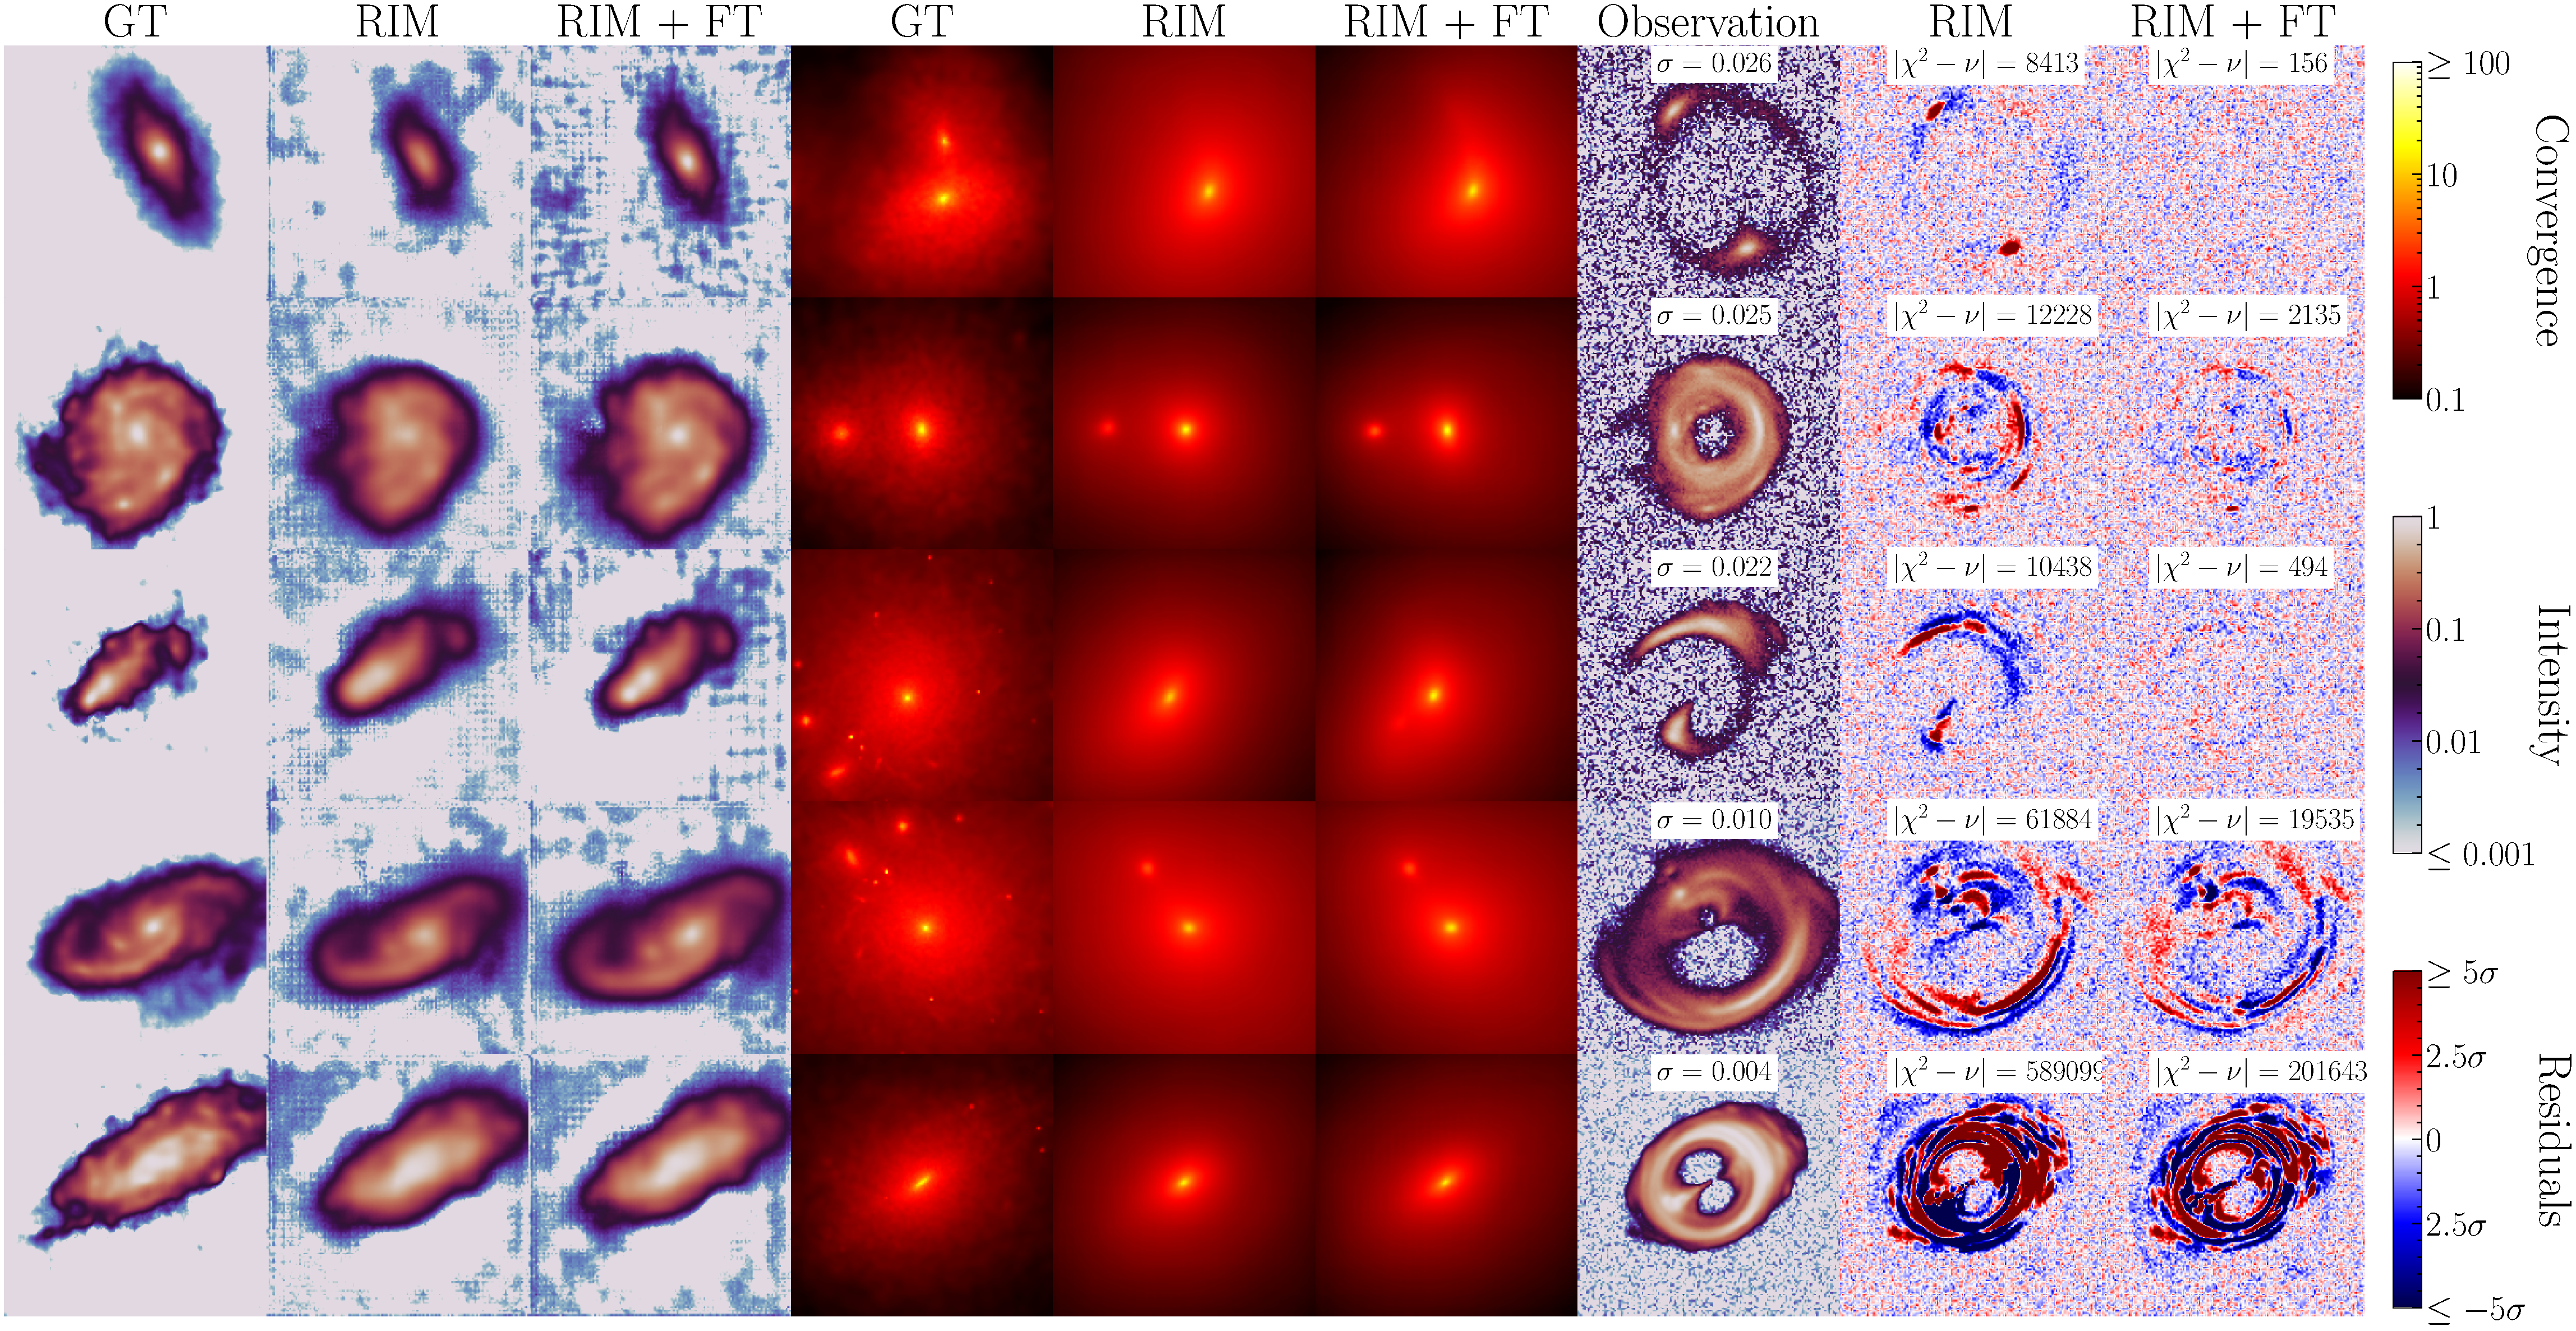
\includegraphics[width=\linewidth]{figures/rim_map_wrt_snr.pdf}};
                \draw[-latex] (-8.5, 3.5) -- (-8.5, -3.5) node[midway, above, rotate=90] {Increasing SNR};
                \node at (-5.5, 4.5) {\strut Source};
                \node at (-0.75, 4.5) {\strut Convergence};
                \node at (5, 4.5) {\strut Residuals};
        \end{tikzpicture}
        \caption{
        Comparison between baseline (RIM) and fine-tuned (RIM+FT) reconstructions for gravitational lensing systems from the test set (GT).
        From top to bottom, we increase SNR. 
        }
        \label{fig:increasing SNR}
\end{figure}
%\vfill\null 

\subsection{Quality of the Reconstructions}\label{sec:quality of reconstructions}

\begin{figure}[H]
        \centering
        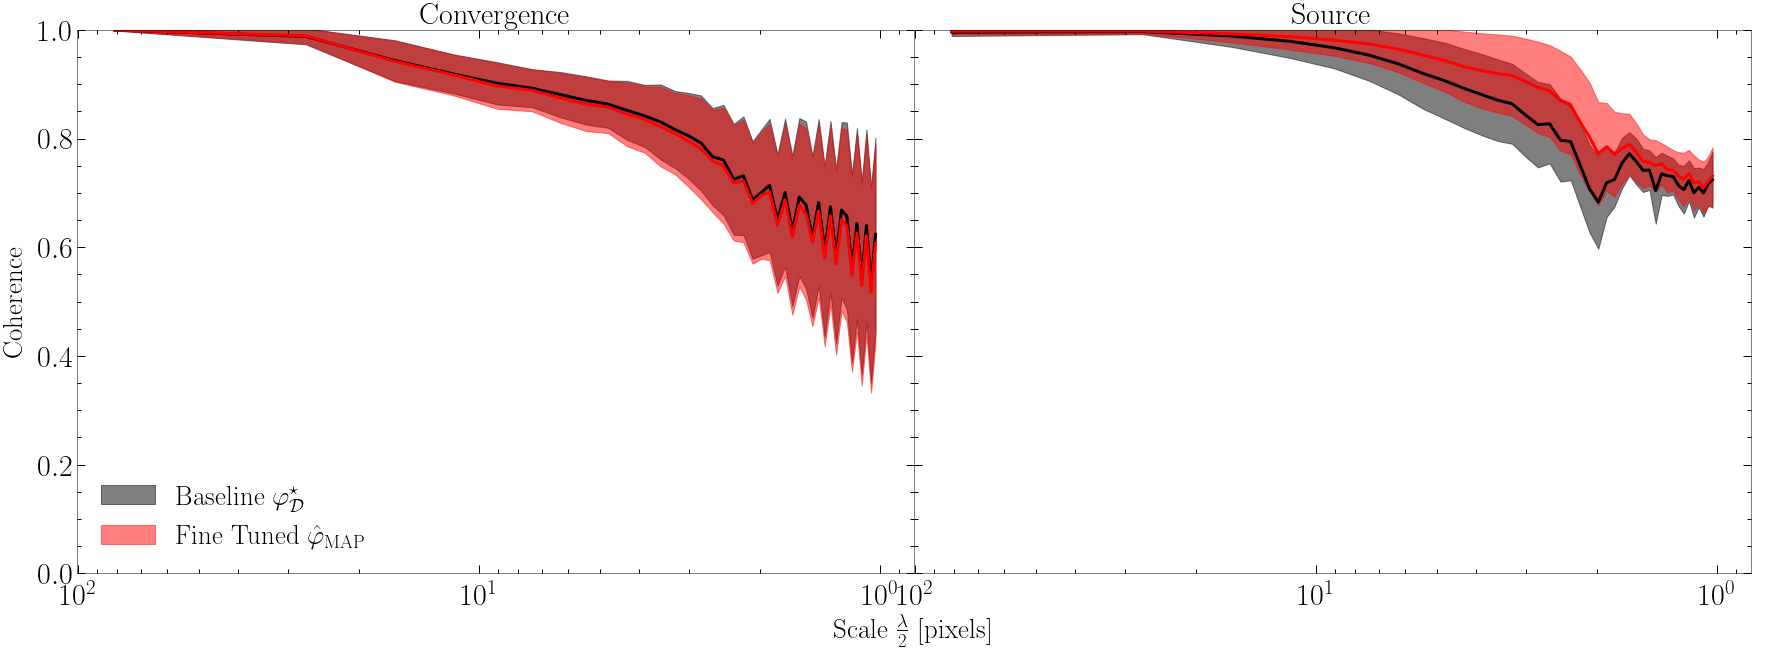
\includegraphics[width=0.8\linewidth]{figures/coherence_spectrum}
        \caption{Statistics of the coherence spectrum on the test set. The solid line is the average 
        coherence. The transparent region is the $68\%$ confidence interval. The fine-tuning 
        procedure yields a noticeable improvement on the coherence of the source at all frequencies.}
        \label{fig:coherence}
\end{figure}


In addition to a visual inspection of the reconstructed sources 
and convergences, we compute 
the coherence spectrum to quantitatively assess the quality of the reconstructions
\begin{equation}\label{eq:coherence} 
        \gamma(k) = \frac{P_{12}(k)}{\sqrt{P_{11}(k) P_{22}(k)}} \, .
\end{equation}

Here, $P_{ij}(k)$ is the cross power spectrum of images $i$ and $j$ at 
the wavenumber $k$. Figure \ref{fig:coherence} shows the mean value and the $68\%$ inclusion interval of $\gamma(k)$ 
for the convergence and source maps in a test set of 3000 examples. 
The fine-tuning 
procedure, shown in red, is able to significantly improve the coherence of the baseline background 
source, shown in black, at all scales. 
The coherence spectrum of the convergence sees a slight improvement due to the fine-tuning procedure.
Still, we note that many examples in the dataset exhibit significant 
improvement, which we illustrate in Figure \ref{fig:main figure}.
%In this case, the observed lensed image exhibits a large deflection in 
%its eastern arc which indicates the presence of a massive object --- in this 
%case a dark matter subhalo. The fine-tuning procedure is able to recover 
%this subhalo because of its strong signal in the lensed image.


\section{Conclusion}\label{sec:conclusion}
The results obtained here demonstrate the effectiveness of machine learning methods, specifically a recurrent inference machine, for inferring pixelated maps of the distribution of mass in lensing galaxies and the distribution of surface brightness in the background galaxies. Since this is a heavily under-constrained problem, stringent priors are needed to avoid overfitting the data, a task that has traditionally been difficult to accomplish with traditional statistical models \citep[e.g., ][]{Saha1997}. The model proposed here can implicitly learn these priors from a set of training data. 

The fine-tuning step that we propose in this work is a general procedure (i.e.\ not specific to our model or problem), which enables us to exploit a diagonal second-order Laplace approximation of the implicit prior learned by a baseline estimator during pre-training. We use fine-tuning in order to significantly improve this baseline estimator (i.e., a better MAP estimate), by using the likelihood of the data and the EWC prior. In the context of our work, we find that fine-tuning has a limiting --- or threshold --- behavior, which we speculate is due to the limited expressivity of the neural network and its inductive biases learned during pre-training.

The flexible and expressive form of the reconstructions shown in this work means that, in principle, any lensing system (e.g., a single simple galaxy or a group of complex galaxies) could be analyzed by this model, without any need for pre-determining the model parameterization. This is of high value given the diversity of observed lensing systems, and their relevance for constraining astrophysical and cosmological parameters. 

Perhaps the most important limitation of the method is the fact that, in its current form, the model only provides point estimates of the parameters of interest. Quantifying the posteriors of such high-dimensional data will require an efficient and accurate generative process \citep[e.g., see ][]{Adam:22a}, which we plan to explore and develop in future works.

\section*{Software and data}
The source code, as well as the various scripts and parameters used to 
produce the model and results is available as open-source software 
under the package \texttt{Censai}\footnote{
\href{https://github.com/AlexandreAdam/Censai}{

\includegraphics[scale=0.25]{figures/GitHub-Mark-32px.png}
https://github.com/AlexandreAdam/Censai}}. 
The model parameters, as well as convergence maps used to train 
these models and the test set examples and reconstructions results are also available as open-source datasets hosted by Zenodo\footnote{\href{https://doi.org/10.5281/zenodo.6555463}
{
\includegraphics[scale=0.1]{figures/zenodo}
https://doi.org/10.5281/zenodo.6555463}}. This research made use of \texttt{Tensorflow} \citep{tensorflow}, 
\texttt{Tensorflow-Probability} \citep{tensorflow-probability}, 
\texttt{Numpy} \citep{numpy}, 
\texttt{Scipy} \citep{scipy}, 
\texttt{Matplotlib} \citep{matplotlib}, 
\texttt{Scikit-image} \citep{scikit-image}, 
\texttt{IPython} \citep{ipython}, 
\texttt{Pandas} \citep{pandas1,pandas2}, 
\texttt{Scikit-learn} \citep{scikit-learn}, 
\texttt{Astropy} \citep{astropy:2013,astropy:2018} 
and \texttt{GalSim} \citep{galsim}.

\section*{Acknowledgements}

This research was made possible by a generous donation by Eric and Wendy Schmidt with the recommendation of the Schmidt Futures Foundation.

We would like to thank Ronan Legin for fruitful discussions and insights about training the neural network. We would also like to thank Max Welling for insightful comments on our work.  The work is in part supported by computational resources provided by Calcul Quebec, Compute Canada and the Digital Research Alliance of Canada. Y.H. and L.P. acknowledge support from the National Sciences and Engineering Council of Canada grant RGPIN-2020-05102, the Fonds de recherche du Québec grant 2022-NC-301305 and 300397, and the Canada Research Chairs Program. A.A. was supported by an IVADO Excellence Scholarship.




{\footnotesize
  \bibliography{intro_bib,censai_bib}
}

  \appendix
   %\chapter{L'équation de la lentille}
% Plan pour cette section: Dériver eq de la lentille et alpha
% Intro général: deflection de la lumière
%% Approcha a l'intro -> contexte historique à notre pensée sur la déviation de la lumière
%%% Réfraction 
%%%% Ptolémé (Optic, Grèce Antique)
%%%% Ibn Sahl (c. 940 - 1000)
%%%% Snell (1621)-Descartes(1637)
%%%% Principe de Fermat pour expliquer ce phénomène (lettre en 1657, mémoire en 1662)
%%%% Euler (1744) - Lagrange (1760) -> Principe de moindre action et sa solution
%%%% Équations de Maxwell (1861)

%%% déviation de la lumière par la gravité
%%%% Soldner, J. G. v. (1801–1804). "On the deflection of a light ray from its rectilinear motion, by the attraction of a celestial body at which it nearly passes by". Berliner Astronomisches Jahrbuch: 161–172.
%%%% Einstein 1911
%%%% Einstein 1915 (GR)
%%%% Eddington takes photograph of eclipse 1919
%%%% 1936 letter from Einstein at the request of 
%%%% Fritz Zwicky is first to postulate grav lensing idea in 1937i Zwicky, F. (1937) Nebulae as gravitational lenses. Physical Review, 51 (4). p. 290. ISSN 0031-899X
%%%% 1964 Refsdal (H0 and possibility to measure mass)
%%%%%% (Shapiro time delay (1964))
%%%% Fisrt gravitational lens discovered 1979 (double imaged quasar) https://www.nature.com/articles/279381a0
%%%% Then explosions of studies durings the 2000s on how to model things.

%%% Dark matter 
%%%% Zwicky 1933
%%%% Lambda CDM?
%%%% 

% Copied from https://royalsocietypublishing.org/doi/10.1098/rsta.2009.0209
%Henry Cavendish in 1784 is credited with the first (unpublished) calculation of the deflection angle 
%δ of a corpuscular light ray following a hyperbolic trajectory and the origin of the 
%(Newtonian) equation δ=2GM/Rc2. Subsequently, von Soldner (1804) published a similar calculation 
%deriving a deflection of 0.84 arcsec for stars viewed close to the limb of the Sun.

%Le principe de Fermat énonce que la trajectoire de la lumière, ou d'un 
%photon, doit suivre une trajectoire qui extrémise la durée de la trajectoire. 
%Ce principe mathématique, qui est un exemple du principe plus général de moindre action 
%développé par Lagrange en 1756, permet de décrire la trajectoire de la lumière 
%par l'entremise d'un simple indice $n$ (indice de réfraction) dans 
%lequel se cache toute la physique microscopique (ou macroscopique) 
%d'où émerge le phénomène qui nous intéresse. 


%L'expédition organisée par sir Arthur Eddington
%avait pour but d'observer 
%l'éclipse totale du 29 mai 1919 à partir de l'île de Prìncipe 
%dans le golfe de Guinée et de Sobral au nord du Brésil 
%\citep{Eddington1919}. Les photographes de l'éclipses prisent , bien qu'imprécises, 
%ont permis de valider la prédiction d'Einstein faite 
%en 1911 que la position observée d'une étoile serait déplacée de 
%$\delta \theta \approx 1.75'' \frac{R}{R_\odot}$ 
%durant une eclipse \citep{Dyson1920}, soit 2 fois plus 
%que ce qui est prédit par la théorie newtonienne.

%Dans l'intérêt de rendre ce manuscrit complet, je dérive à partir de principes 
%premier les deux équations centrales qui nous permettent 
%d'étudier les lentilles gravitationnelles.
Dans cette section, je dérive les équations centrales qui nous permettent 
d'étudier les lentilles gravitationnelles de type galaxie-galaxie.
Des traitements similaires 
peuvent être trouvé dans les manuels de références de \citet{Meneghetti2013} et 
\citet{Carroll2003}.


Supposons qu'un photon est sur une trajectoire parallèle à l'axe de 
visée $\mathbf{e}_{\parallel}$ d'un observateur sur Terre. 
Supposons de plus qu'un champ gravitationnel $\Phi$ a pour effet de courber la 
trajectoire de ce photon entre son point d'origine $A$ et son point d'arrivé $B$.
On définit l'angle de déviation comme la déviation totale de cette trajectoire 
dans la direction perpendiculaire à l'axe de visée de l'observateur. 
Selon nos suppositions, cette déviation s'écrit
\begin{equation}\label{eq:alpha}
        \boldsymbol{ \alpha} = - \int_{\lambda_A}^{\lambda_B} \ddot{\mathbf{x}} \times \mathbf{e}_{\parallel} d\lambda,
\end{equation}
où $\lambda$ paramétrise la trajectoire du photon, et $\mathbf{x}$ est la positon du photon. 
Le signe négatif nous indique qu'on prend la perspective de l'observateur. 

Pour résoudre l'intégrale \eqref{eq:alpha}, on doit déterminer la forme de 
la trajectoire des photons dans un champ gravitationnel caractérisé par un 
indice de réfraction $n$. 
Le principe de Fermat stipule que la lumière suit une trajectoire qui extrémise
la durée du parcours entre deux points. 
Dans le language du calcul 
des variations, la variation de la durée $T$ s'écrit
\begin{equation}\label{eq:Fermat}
        \delta T =  \delta \int_{A}^{B} n(\mathbf{x}(\ell)) \frac{d\ell}{c}= 0,
\end{equation}
où $\ell$ est un élément de longueur sur la trajectoire.
Pour déterminer l'indice de réfraction du champ gravitationnel d'une galaxie, 
on doit utiliser le formalisme de la relativité générale. Selon le principe 
d'équivalence (fort), 
l'effet d'un champ gravitationnel est localement 
indistinguable d'une accélération causée par la courbure 
de l'espace-temps décrit par 
une métrique $g_{\mu \nu}$. 
La trajectoire d'un photon se trouve alors en cherchant 
les géodésiques de cet espace-temps. 
On fait l'approximation 
que le potentiel $\Phi$ d'une galaxie est celui d'un gas parfait, c'est-à-dire 
qu'il satisfait une équation de Poisson
\begin{equation}\label{eq:Poisson}
       \grad^{2}\Phi = 4\pi G \rho .
\end{equation} 
Dans la limite où ce potentiel est faible $\displaystyle \frac{2\Phi}{c^{2}} \ll 1$, la 
métrique $g_{\mu \nu}$ est décrite par une expansion au premier ordre autour de la 
métrique de Minkowsky $\eta_{\mu\nu}$
\begin{equation}\label{eq:metrique}
        ds^2 = g_{\mu\nu}dx^{\mu}dx^{\nu} \approx \left( 1 + \frac{2\Phi}{c^{2}} \right)c^{2}dt^{2} - \left( 1 - \frac{2\Phi}{c^{2}} \right)d\mathbf{x}^{2}.
\end{equation} 
Ici, j'ai choisit arbitrairement la signature $(+,-,-,-)$ pour la métrique.
Puisqu'un photon suit une géodésique de l'espace-temps $ds^{2} = 0$, on peut déterminer 
$n$ en réarrengeant l'équation \eqref{eq:metrique}
\begin{equation}\label{eq:n}
        n = c \left( \frac{\lVert d \mathbf{x} \rVert}{dt}  \right)^{-1} \approx  1 - \frac{2\Phi}{c^{2}}.
\end{equation} 
En réécrivant l'élément de longueur $d\ell$ en terme du 
paramètre de la trajectoire $\lambda$
\begin{equation}\label{eq:ell}
        d\ell = \left\lVert\frac{d  \mathbf{x} }{d\lambda} \right\rVert d\lambda,
\end{equation} 
on peut réécrire l'équation \eqref{eq:Fermat} sous la forme
\begin{equation}\label{eq:Fermat2}
        \delta \int_{\lambda_A}^{\lambda_B} n(\mathbf{x}) \lVert \mathbf{\dot{x}} \rVert d\lambda = 0.
\end{equation} 
Par correspondance avec la fonctionnelle de l'action 
$J(x) = \int_{\lambda_0}^{\lambda_1} \mathcal{L}(\lambda,\, x,\,\dot{x}) d\lambda$ 
on trouve que 
le lagrangien de la trajectoire s'écrit 
\begin{equation}\label{eq:lagrangien}
        \mathcal{L} = n(\mathbf{x})  \sqrt{\dot{x}^{2}}.
\end{equation} 
La trajectoire qui satisfait \eqref{eq:Fermat} 
est une solution des équations d'Euler-Lagrange
\begin{equation}\label{eq:EulerLagrange}
        \frac{d }{d \lambda} \frac{\partial \mathcal{L}}{\partial \dot{\mathbf{x}}} - \frac{\partial \mathcal{L}}{\partial \mathbf{x}} = 0.
\end{equation} 
On a donc
\begin{equation}\label{eq:EulerLagrange2}
        \frac{d }{d \lambda} n \frac{\dot{\mathbf{x}}}{\lVert \dot{\mathbf{x}} \rVert}- \lVert \dot{\mathbf{x}} \rVert \grad n = 0 ,
\end{equation} 
Puisque le choix du paramètres $\lambda$ est libre, on peut le choisir tel 
que $\lVert \dot{\mathbf{x}} \rVert = 1$ en tout point de la trajectoire. Ainsi,
\begin{equation}\label{eq:EulerLagrange3}
\begin{aligned}
        \frac{d }{d \lambda} n \dot{\mathbf{x}} -  \grad n &= 0 \\
        \implies n \ddot{\mathbf{x}} + (\grad n \cdot \dot{\mathbf{x}}) \dot{\mathbf{x}} - \grad n &= 0
\end{aligned}
\end{equation} 

À ce point de la dérivation, on utilise l'approximation de Born. 
C'est-à-dire qu'on approxime la trajectoire 
du photon comme une ligne droite sur l'axe de visée $\mathbf{e}_{\parallel}$. 
Cette approximation est justfiée 
dans le contexte des lentilles gravitationnelles de type galaxie-galaxie, 
puisque les angles de déviation sont généralement de 
l'ordre de l'arcseconde ou plus petit. 
Comme, le vecteur $\dot{\mathbf{x}}$ est tangent à la trajectoire du photon, 
on obtient
\begin{equation}\label{eq:sol}
        \ddot{\mathbf{x}} \times \mathbf{e}_{\parallel} = \frac{1}{n} \grad_\perp n = \grad_\perp \log n
        \approx -\frac{2}{c^{2}}\grad_{\perp} \Phi
\end{equation} 
On note que le facteur 2 qui apparaît dans l'équation \eqref{eq:sol} est un 
effet qui vient de la relativité générale. Ce facteur corrige la solution 
que l'on aurait obtenu avec une dérivation classique (newtonienne).


On est maintenant en mesure de calculer l'angle de déviation. 
J'introduit le paramètre d'impact $\boldsymbol{\xi}$ qui est la distance perpendiculaire entre 
la position d'origine du photon sur le plan de la lentille  
et l'axe de visé. Cette distance peut être interprétée à l'aide du schéma dans la 
Figure \ref{fig:cartoon}.
Dans le cas où le potentiel est généré par une masse $M$ ponctuelle, ç.-à-d. qu'on 
suppose $\rho = M\delta^{3}(\mathbf{x})$ où $\delta $ est la fonction delta de Dirac, 
alors le potentiel qui satisfait l'équation de Poisson est 
la fonction de Green 
$\displaystyle \Phi = -\frac{GM}{\sqrt{ \xi^{2} + z^{2}}}$, où $z$ est la coordonné 
sur l'axe de visée. L'équation \eqref{eq:alpha} se réécrit finalement
\begin{align}
\nonumber
        \boldsymbol{ \alpha}(\boldsymbol{ \xi} ) &= -\frac{2GM}{c^{2}} \int_{-\infty }^{\infty }  \frac{\partial}{\partial \boldsymbol{\xi} }\frac{1}{(\xi^{2} + z^{2})^{1/2}}dz \\
\nonumber
        &= \frac{2GM}{c^{2}} \boldsymbol{ \xi}  \int_{-\infty }^{\infty } \frac{1}{(\xi^{2} + z^{2})^{3/2}}dz  \\
\label{eq:deflection approx}
        \implies \boldsymbol{ \alpha}(\boldsymbol{ \xi})  &= \frac{4GM}{c^{2}  \xi^{2} } \boldsymbol{ \xi}
\end{align} 
Cette solution se généralise naturellement à un profil de masse quelconque en assumant 
qu'il s'exprime comme une somme d'élément de masses $dm = \Sigma d^{2}\boldsymbol{ \xi}'$ 
où $\Sigma = \int \rho dz$ est un densité surfacique de masse. 
L'angle de déviation total mesuré à un point $\boldsymbol{\xi} $ est alors une convolution 
sur tout le plan de la lentille (mince) puisque l'équation \eqref{eq:deflection approx} dépend 
linairement de la masse $M$:
\begin{equation}\label{eq:alpha physique}
        \boldsymbol{ \alpha} (\boldsymbol{ \xi} ) = \frac{4 G}{c^{2}} 
        \int_{\mathbb{R}^{2}} \Sigma (\boldsymbol{ \xi} ')
        \frac{\boldsymbol{ \xi}  - \boldsymbol{ \xi} '}{\lVert \boldsymbol{ \xi}  - \boldsymbol{ \xi} ' \rVert^{2}}d^{2}\boldsymbol{ \xi} '
\end{equation} 

Cette déviation nous permet alors de relier le plan de la lentille et le plan de la source. 
Pour ce faire, on doit retrouver la position angulaire 
d'un point lumineux à la source $\boldsymbol{\beta}$ à partir de sa position angulaire
observée $\boldsymbol{ \theta} $ et de nos connaissances sur la déviation $\boldsymbol{ \alpha}$. 
On assume que les distances $D_{\ell}$, $D_s$ et $D_{\ell s}$ sont beaucoup 
plus grandes que les distances perpendiculaires $\boldsymbol{ \xi} $ ou $\boldsymbol{ \eta} $ 
(voir figure \ref{fig:cartoon}). 
Pour les objets qui nous intéresses, les distances parallèles à l'axe de visée sont généralement 
de l'ordre du Gpc, alors que les distances perpendiculaire sont généralement 
de l'ordre du kpc, soit 6 ordres de grandeurs de différences.
Ainsi, on peut faire l'argument géométrique
\begin{align}
\nonumber
       D_{s} \boldsymbol{ \theta} &= \boldsymbol{ \eta}' \\   
\nonumber
       D_{s} \boldsymbol{ \beta} &= \boldsymbol{ \eta} \\   
\nonumber
       D_{\ell s} \boldsymbol{ \alpha} &= \boldsymbol{ \eta}' - \boldsymbol{ \eta}  \\   
\label{eq:lens equation}
       \implies D_s \boldsymbol{ \beta} &= D_s \boldsymbol{ \theta} - D_{\ell s} \boldsymbol{ \alpha}   
\end{align} 
C'est l'équation maîtresse qui nous permet de tracer les rayons lumineux d'une source 
vers un détecteur fictif dans nos simulations.

Lorsqu'on étudie des images, il est généralement plus utile de travailler directement à partir 
du système de coordonnées angulaires $\boldsymbol{ \theta}$ plutôt que des dimensions physiques 
$\boldsymbol{ \xi}$ qui requièrent une caractérisation précise de la distance entre 
l'observateur et la lentille $\boldsymbol{ \xi}  = D_\ell \boldsymbol{ \theta} $.
On peut absorber cette distances dans un préfacteur qui rend les expressions 
\eqref{eq:alpha physique} et \eqref{eq:lens equation} adimensionnelles.
On introduit la densité critique 
\begin{equation}\label{eq:densite critique}
        \Sigma_c = \frac{c^2}{4 \pi G}\frac{D_{s}}{D_{\ell s} D_\ell}
\end{equation} 
et la convergence $\displaystyle \kappa(\boldsymbol{ \theta} ) = \frac{\Sigma(\boldsymbol{ \theta})}{\Sigma_c}$, 
de sortes qu'on obtient l'angle réduit
\begin{equation}\label{eq:alpha adim}
        \hat{\boldsymbol{ \alpha}} (\boldsymbol{ \theta}) = \frac{1}{\pi}\int_{\mathbb{R}^{2}} \kappa(\boldsymbol{ \theta} )
        \frac{\boldsymbol{ \theta} - \boldsymbol{ \theta}'  }{\lVert \boldsymbol{ \theta} - \boldsymbol{ \theta}' \rVert  } d^{2}\boldsymbol{ \theta}'   
\end{equation} 
qui satisfait
\begin{equation}\label{eq:lens equation adim}
        \boldsymbol{ \beta} = \boldsymbol{ \theta} - \hat{\boldsymbol{ \alpha}}(\boldsymbol{ \theta})    
\end{equation}

\begin{figure}[H]
        \centering
        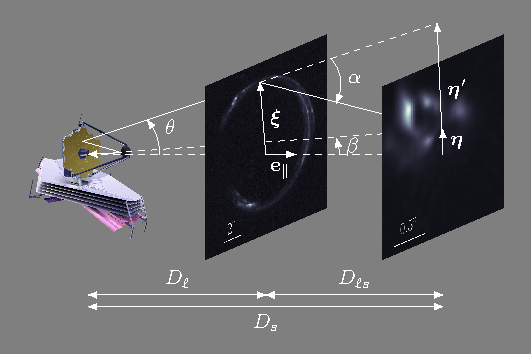
\includegraphics[width=0.7\textwidth]{figures/lensing_cartoon}
        \caption{Schéma d'une lentille gravitationnelle.}
        \label{fig:cartoon}
\end{figure}





   %\chapter{Distance du diamètre angulaire}

Étant donné les distances de l'ordre du Gpc entre une lentille gravitationnelles 
et un observateur situé 
dans la Voie Lactée (sur Terre par exemple),
on doit tenir compte du phénomène de l'expansion de l'Univers et en général de sa courbure 
pour déterminer la trajectoire réelle des photons. 
C'est pourquoi on utilise plutôt 
le concept de distance du diamètre angulaire (de l'anglais \textit{angular diameter distance}) 
lorsqu'on mesure les distances le long de l'axe de visée. 
Cette distance est définit par 
la relation euclidienne entre une longueur $\ell$ et un angle observé $\theta$:
\begin{equation}\label{eq:D}
        D \equiv \frac{\ell}{\theta}
\end{equation} 
Pour un espace euclidien (plat et statique), les distances $D$ et $\ell$ 
sont toujours décrites par la norme euclidienne $\lVert \cdot \rVert_2$, 
ce peut importe la distance qui sépare l'observateur à l'objet de taille 
$\ell$.
Pour un Univers en expansion et possiblement courbe, on doit changer la 
définition de $D$ et $\ell$ pour satisfaire la relation \eqref{eq:D}, cruciale 
à la dérivation de l'équation de la lentille.

On part du principe cosmologique, qui stipule que l'Univers est homogène et isotrope.
%Partant du principe cosmologique selon lequel l'Univers est isotrope et homogène, 
%il suit que seul une métrique avec une symétrie spatial maximale peut décrire l'Univers. 
%de Friedmann-Lemaître-Robertson-Walker\footnote{Voir section 13.5 de \citet{Weinberg1972} pour une discussion 
%de l'unicité de cette métrique.}:
\begin{equation}\label{eq:FLRW}
        ds^{2} = c dt^{2} - a^{2}(t) \left( \frac{dr^{2}}{1 - kr^{2}} + r^{2}d\Omega^{2} \right)
\end{equation} 
où $k \in \{-1,0,1\}$ est le paramètre de la courbure et $(r,\theta,\phi)$ sont 
les coordonnées comobiles sphériques.

Redshift
\begin{equation}\label{eq:redshift}
       z = \frac{\lambda_o - \lambda_e}{\lambda_e} 
\end{equation} 
null geodesic 
\begin{equation}\label{eq:}
        \int_{t_e}^{t_o} \frac{c dt}{a(t)} = \int_{0}^{r} \frac{dr}{\sqrt{(1 - kr^{2})}}
\end{equation} 
and light emitted a wavelength away is emitted at $t'_e = t_e = \delta t_e$ et 
$t'_o = t_o + \delta t_o$. 
\begin{equation}\label{eq:}
        \int_{t'_e}^{t'_o} \frac{c dt}{a(t)} = \int_{0}^{r} \frac{dr}{\sqrt{(1 - kr^{2})}}
\end{equation} 

Implication from $\delta t_e$ and $\delta t_o$ small is
\begin{equation}\label{eq:}
       \frac{\delta t_0}{a_0}  = \frac{\delta t}{a}
\end{equation} 
Since $\delta t = 1/\nu_e$ et $\delta t_o = 1/\nu_o$ then $\nu_e a = \nu_o a_o$

\begin{equation}\label{eq:}
        1  + z = \frac{a_0}{a}
\end{equation} 

La première équation de Friedmann, de la composante $00$ des équations d'Einstein
\begin{equation}\label{eq:Friedmann1}
        \frac{\dot{a}^{2 + kc^2}}{a^{2}} = \frac{8 \pi G \rho + \Lambda c^2}{3}
\end{equation} 
La seconde, de la trace de la composante spatiale
\begin{equation}\label{eq:Friedmann}
        \frac{\ddot{a}}{a} = -\frac{4 \pi G}{3} \left( \rho + \frac{3p}{c^{2}} \right) + \frac{\Lambda c^{2}}{3}
\end{equation} 
En terme des paramètres cosmologiques, on a $\rho_c = \frac{3H^{2}}{8 \pi G}$ et $\Omega \equiv \frac{\rho}{\rho_c}$
\begin{equation}\label{eq:}
        \frac{H^{2}}{H_0^{2}} = \Omega_{R} a^{-4} + \Omega_M a^{-3} + \Omega_k a^{-2} + \Omega_\Lambda
\end{equation} 
déterminé en terme de $p = w \rho c^{2}$ ($w = 0$ is dust, $w = \frac{1}{3}$ is radiation, $w = -1$ is $\Lambda$). 
$\Omega_k = 1 - \Omega_0 = 1 - \Omega_M - \Omega_R - \Omega_\Lambda$. In a flat Universe, $\Omega_k = 0$.

%On doit maintenant déterminer comment $\ell$ et $\theta$ se comportent en fonction de 
%la distance. Pour se faire, on doit faire certaines suppositions par rapport 
%à notre Univers. 
%Mon traitement s'inspire des dérivations qu'on peut trouver 
%dans les textes de références de 
%\citet{Dodelson2003}, \citet{Carroll2003}, \citet{Rindler2006} et 
%\citet{Weinberg2008}.


%Nature de l'argument: 
%1. Pour résoudre les équations d'Einstein, on doit faire certaines supposition sur les symmétries 
%de l'Univers
%2. Isotropie et homogénéité suivent des observations de notres Univers local (galaxy count in sphere).
%3. Asymmétrie temporelle -> Hubble + Planck (et autres observable, pourrait être mentionné rapidement, comme les niveaux 
%d'abondances chimiques etc).
%4. Dériver rapidement la forme d'une distance comobile, ce qui mène à la distance du diamètre angulaire 
% en terme de H_0, Omega et potentiellement mentionner qu'on assume un Univers plat.
%5. End with adimensional equations.

%Il est généralement plaisant de commencer cette dérivation en statuant le postulat de 
%Copernic: \textit{il n'existe aucun point de vue privilégié dans l'Univers}. Dans un sens, 
%ce postulat nous encourage à se mettre dans la peau d'un être conscient observant le ciel 
%à partir d'une autre planète, où même d'une autre galaxie. Cet observateur devrait être en 
%mesure de parvenir aux même conclusions que nous sur la structure générale de l'Univers. 
%Il est tout à fait raisonnable de protester 
%que l'environnement proche de cet observateur soit bien différent 
%du notre. Mais, en portant ses observations à grande échelle où les différences locales 
%entre différentes galaxies ou systèmes planétaires disparaissent dans une agrégation statistique, 
%alors les conclusions de cet observateur devrait s'accorder avec nos conclusions.

%Ceci nous mène à postuler le principe cosmologique: 
%\textit{l'Univers est spatialement homogène et localement isotrope}.
%Ce principe est une reformulatione du postulat de Copernic. L'isotropie 
%locale encode le fait que l'espace est le même peut importe la direction 
%que l'on choisit pour l'observer. La meilleur évidence pour l'isotropie est 
%le fond diffus cosmologique, soit l'émission caractéristique d'un corps 
%noir de température $T = 2.725\, \mathrm{K}$ avec une racine de l'écart quadratique 
%moyen de seulement $\sigma_T = 18\,\mu \mathrm{K}$.
%\begin{figure}[H]
        %\centering
        %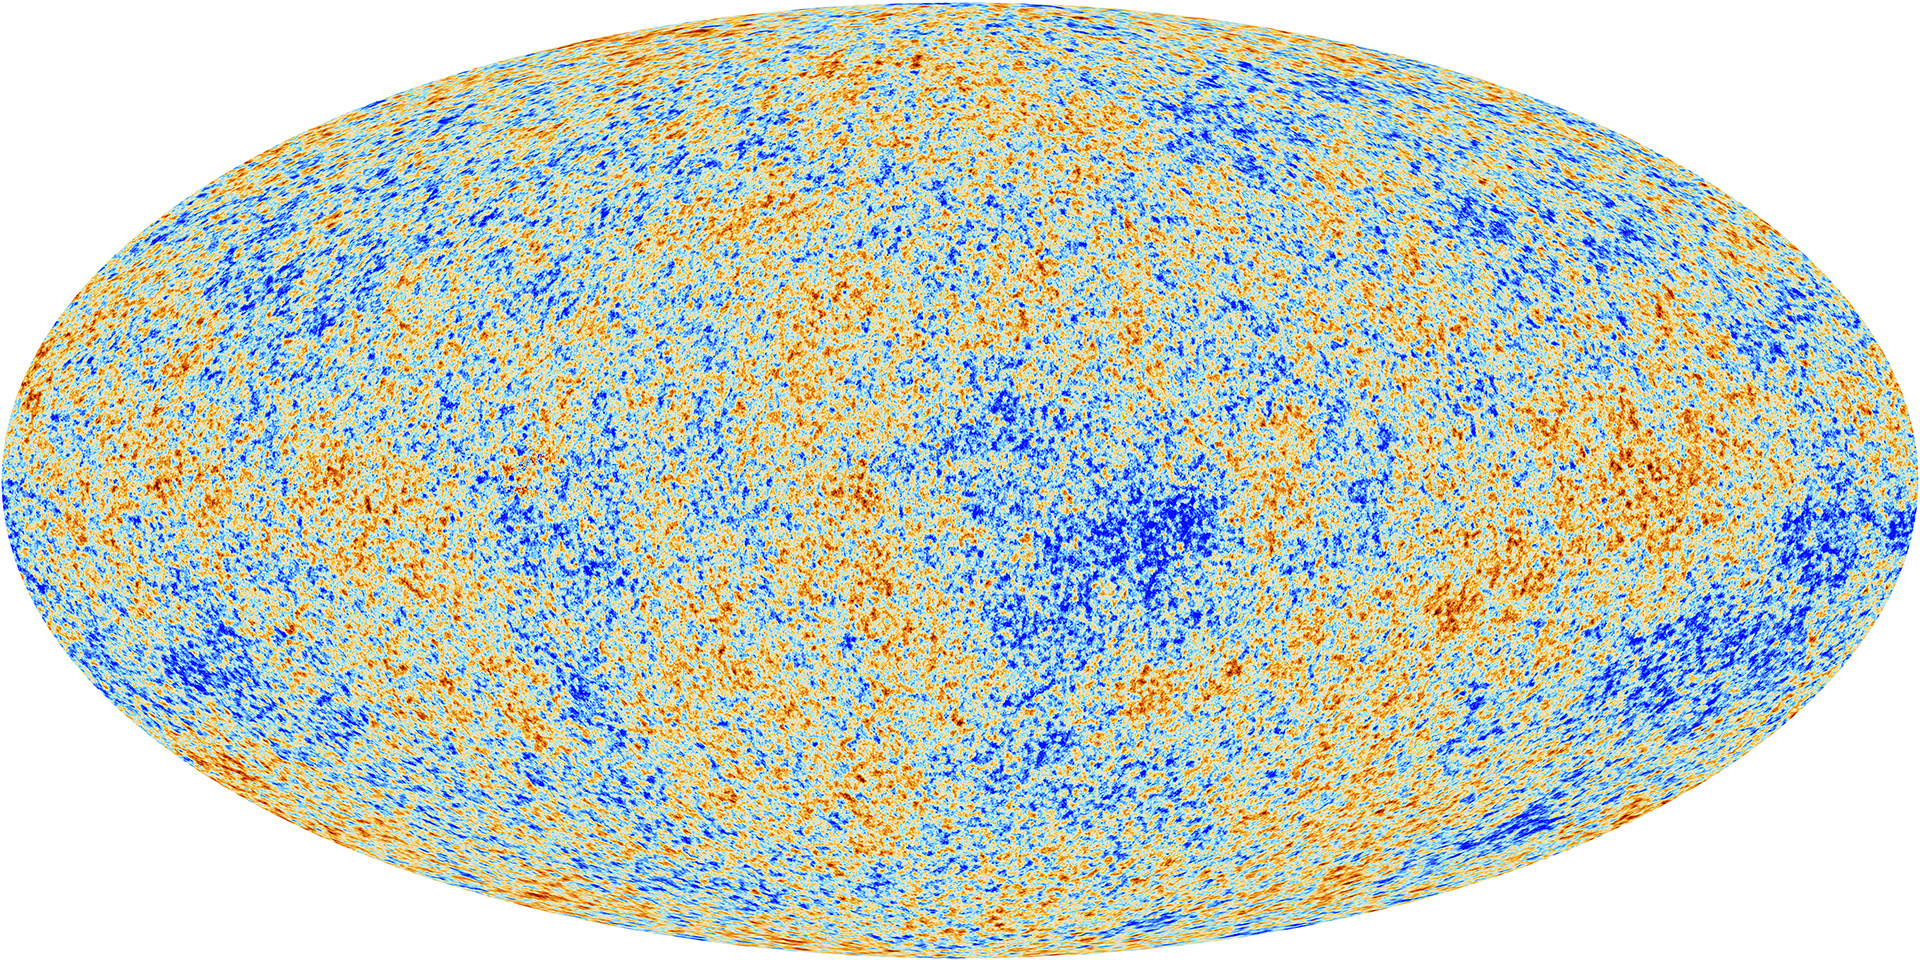
\includegraphics[width=0.8\textwidth]{figures/Planck_CMB}
        %\caption{Carte de la température du fond diffus cosmologique. La couleur indique 
        %les déviation de la température du corps noir. Ces déviations sont extrêmements petites, 
%supportant l'argument que l'Univers est localement isotropique. Crédit: \textit{ESA and the Planck Collaboration}.}
        %\label{fig:}
%\end{figure}

%L'homogénéité encode le fait que la métrique qui décrit l'espace-temps doit être la même 
%peut importe l'endroit dans l'Univers où l'observateur se situe. C'est une affirmation qui 
%concerne la distribution de matière et d'énergie dans l'Univers. Un Univers est homogène dans 
%le sens où la distribution de la matière et d'énergie est elle aussi homogène. Ainsi, 
%par les équations de champs d'Einstein qui relient le tenseur d'énergie-impulsion 
%à la courbure de l'espace-temps, on peut voir comment une affirmation qui concerne 
%la métrique implique immédiatement certaines propriétés pour la matière:
%\begin{equation}\label{eq:EFE}
        %G_{\mu\nu} = \frac{8 \pi G}{c^{4}} T_{\mu \nu}
%\end{equation} 
%Une étude de la distribution des galaxies dans l'Univers proche renforce se point, où 
%on remarque que la distribution de galaxies à l'intérieurs de sphères plus grande que 
%$r = 40\, \mathrm{Mpc}$ est étonnamment homogène. Gaussian distribution.

%metrique FLRW
%assume univers plat (k=0)
%distance comobile -> ell
%redshift
%distance angulaire
%\begin{figure}[H]
        %\centering
        %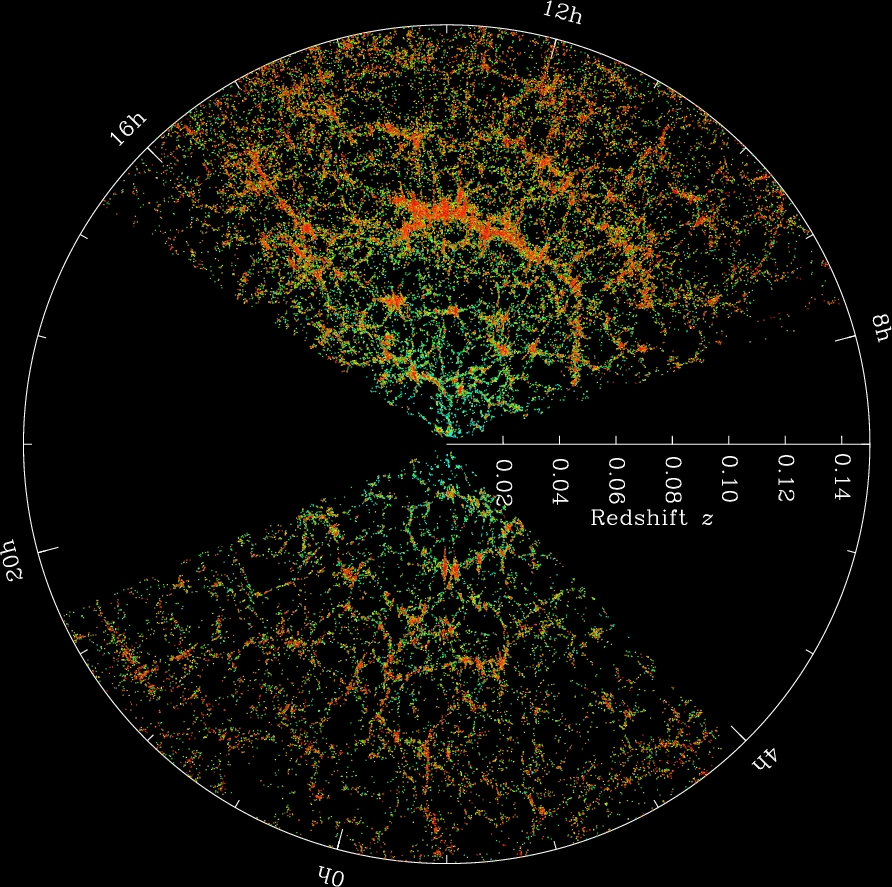
\includegraphics[width=\textwidth]{figures/sdss_universe}
        %\caption{Carte des galaxies prise par le Sloan Digital Sky Survey telescope montrant 
        %le niveau d'homogénéité et d'isotropie de l'Univers local. Chaque point est 
        %coloré par le niveau de densité local.}
        %\label{fig:sdss}
%\end{figure}


%Les symmétries encode une métrique qui est maximalement symmétrique au niveau spatial. On encode 
%l'évolution spatiale avec la facteur $a(t)$. On doit encore régler la question de la courbue de 
%l'espace. En fait, les symmétries du principe cosmologique sont agnostiques sur cette question, 
%de sorte qu'on doit encore faire un postulat.



  \chapter{Elastic Weight Consolidation}\label{ap:ewc}

Suppose we are given a training set $\mathcal{D}$ and a test task $\mathcal{T}$. The 
posterior of the RIM parameters $\mathcal{\varphi}$ can be rewritten using the Bayes rule as
\begin{equation}
        p(\varphi \mid \mathcal{D},\, \mathcal{T}) = 
        \frac{p(\mathcal{T} \mid \mathcal{D},\, \varphi) p(\varphi \mid \mathcal{D})}
        {p(\mathcal{T} \mid \mathcal{D})}.
\end{equation} 
We suppose that $\varphi$ encode 
information about $\mathcal{D}$, while $\mathcal{T}$ was unseen by $\varphi$. 
It follows that 
$\mathcal{T}$ and $\mathcal{D}$ are conditionally independent when given $\varphi$. 
We do not make the stronger assumption that $\mathcal{D}$ and $\mathcal{T}$ 
are completely independent. In fact, such an assumption 
would contradict the premiss of our work that building a 
dataset $\mathcal{D}$ can inform a machine (RIM) about
task $\mathcal{T}$ --- or that, more broadly, $\mathcal{D}$ 
contains information about $\mathcal{T}$.

We rewrite the marginal $p(\mathcal{T} \mid \mathcal{D})$ using the Bayes rule
in order to extract $p(\mathcal{D} \mid \mathcal{T})$, 
the sampling distribution used to compute the Fisher diagonal elements
\begin{equation}
        p(\varphi \mid \mathcal{D},\, \mathcal{T}) = 
\frac{p(\mathcal{T} \mid \varphi) p(\varphi \mid \mathcal{D})}
        {p(\mathcal{D} \mid \mathcal{T})}
        \frac{p(\mathcal{D})}{p(\mathcal{T})}.
\end{equation} 
The log-likelihood $\log p(\mathcal{T} \mid \varphi)$ is equivalent to 
the negative of the loss function for the particular task at hand.
In this work, we assign a uniform probability density to $p(\mathcal{T})$ and $p(\mathcal{D})$ 
in order to ignore them.

We now turn to the prior $p(\varphi \mid \mathcal{D})$, which 
appears as a conditional relative to 
the training dataset. 
We use the Laplace approximation around the maxima $\varphi^{\star}_{\mathcal{D}}$ 
to evaluate the prior,
where $\varphi^{\star}_{\mathcal{D}}$ 
are the trained parameters of the RIM that minimize the empirical risk (equation \eqref{eq:Cost}). 
The Taylor expansion of the prior around this maxima yields
\begin{equation}\label{app:prior}
        \log p(\varphi \mid \mathcal{D}) \approx \log p(\varphi^{\star}_{\mathcal{D}} \mid \mathcal{D}) 
        + \frac{1}{2} (\varphi - \varphi^{\star}_{\mathcal{D}})^{T} 
        \underbrace{
        \bigg(
                \frac{\partial^2 \log p(\varphi \mid \mathcal{D})}{\partial^2 \varphi}\bigg|_{\varphi^{\star}_{\mathcal{D}}}
        \bigg)
}_{\displaystyle \mathbf{H}(\varphi^{\star}_{\mathcal{D}})}
        (\varphi - \varphi^{\star}_{\mathcal{D}}).
\end{equation} 
Since $\varphi^{\star}_{\mathcal{D}}$ is an extrema of the prior, the linear term vanishes. 
The empirical estimate of the negative hessian matrix is the observed Fisher information 
matrix which can be written as
\begin{equation}\label{app:fisher}
        \mathcal{I}(\varphi^{\star}_{\mathcal{D}}) = 
        -\EX_{\mathcal{D} \mid \mathcal{T}} [\mathbf{H}(\varphi^{\star}_{\mathcal{D}})] = 
        \EX_{\mathcal{D}\mid \mathcal{T}}
        \Bigg[
                \Bigg(
                \bigg( 
                        \frac{\partial \log p(\varphi \mid \mathcal{D})}{\partial \varphi}
                \bigg) 
                \bigg( 
                        \frac{\partial \log p(\varphi \mid \mathcal{D})}{\partial \varphi}
                \bigg)^{T}
        \Bigg)
\Bigg|_{\varphi^{\star}_{\mathcal{D}}}\Bigg].
\end{equation} 
The expectation is taken over the sample space $p(\mathcal{D} \mid \mathcal{T})$ since 
the network parameters are held fixed during sampling.
In order to compute the Fisher score, 
we apply the Bayes rule to the prior to extract a loss function,
% \begin{equation} 
%         \log p(\varphi \mid \mathcal{D}) = \log p(\mathcal{D}\mid \varphi) 
%         + \log p(\varphi) - \log p(\mathcal{D}).
% \end{equation} 
% $p(\mathcal{D} \mid \varphi)$ is the negative of a loss function, 
which we take to be 
proportional to the training loss (equation \eqref{eq:Loss}) and the $\chi^2$:
\begin{equation}\label{eq:LossFisher}
        \log p\big(\varphi \mid (\mathbf{x}, \mathbf{y}) = \mathcal{D}\big) \propto -\mathcal{L}_{\varphi}(\mathbf{x}, \mathbf{y}) + \frac{1}{T}\sum_{t=1}^{T}\log p(\mathbf{y} \mid \mathbf{\hat{x}}^{(t)}) - \frac{\ell_2}{2}\lVert \varphi \rVert^2_2
\end{equation} 
% The derivative of $\log p(\varphi)$ remains constant when taking 
% the expectation in \eqref{app:fisher}.
We find in practice the the $\ell_2$ term has little effect on the 
Fisher diagonal and our results. Thus, we set $\ell_2 = 0$.

Since the full Fisher matrix is intractable for a neural network, we approximate the 
quadratic term of the prior with the diagonal of the Fisher matrix following \citet{Kirkpatrick2016}. 
For an optimisation problem, the first term of \eqref{app:prior} is constant. Thus,
the posterior becomes proportional to
\begin{equation}
        \log p(\varphi \mid \mathcal{D}, \mathcal{T}) \propto 
        \log p(\mathcal{T} \mid \varphi ) - 
         \frac{\lambda}{2} 
        \sum_{j}\mathrm{diag}(\mathcal{I}(\varphi^{\star}_{\mathcal{D}}))_{j}(\varphi_j - [\varphi^{\star}_{\mathcal{D}}]_j)^2.
\end{equation} 
The Lagrange multiplier $\lambda$ is introduced to tune our uncertainty about the network parameters 
during fine-tuning.

\chapter{VAE Architecture and optimisation}

For the following architectures, we employ the notion of \textit{level} 
to mean layers in the encoder and the decoder with the same resolution. 
In each level, we place a block of convolutional layers 
before downsampling (encoder) or after upsampling (decoder). These operations 
are done with strided convolutions like in the U-net architecture of the RIM.

\begin{table}[H]
%\begin{minipage}{.5\linewidth} 
        \centering
        \caption{Hyperparameters for the background source VAE.}
        \label{tab:Source VAE}
        \begin{tabular}{cc}
                Parameter & Value \\\hline\hline
                Input preprocessing & $\bbone$ \\
                                    & \\

                \textit{Architecture} & \\
                Levels (encoder and decoder) & 3 \\
                Convolutional layer per level & 2 \\
                Latent space dimension & 32\\
                Hidden Activations & Leaky ReLU \\
                Output Activation & Sigmoid \\
                Filters (first level) & 16 \\
                Filters scaling factor (per level) & 2 \\
                Number of parameters & $3\,567\,361$\\

                           & \\
                \textit{Optimization} & \\
                Optimizer & Adam \\
                Initial learning rate & $10^{-4}$ \\
                Learning rate schedule & Exponential Decay \\
                Decay rate & 0.5 \\
                Decay steps & $30\,000$ \\
                Number of steps & $500\,000$ \\
                $\beta_{\mathrm{max}}$ & 0.1 \\
                Batch size & 20\\
                \hline
        \end{tabular}
\end{table}
%\end{minipage}
%\begin{minipage}{.5\linewidth}
\begin{table}[H]
        \centering
        \caption{Hyperparameters for the convergence VAE.}
        \label{tab:Kappa VAE}
        \begin{tabular}{cc}
                Parameter & Value \\\hline\hline
                Input preprocessing & $\log_{10}$ \\
                              & \\

                \textit{Architecture} & \\
                Levels (encoder and decoder) & 4 \\
                Convolutional layer per level & 1 \\
                Latent space dimension & 16\\
                Hidden Activations & Leaky ReLU \\
                Output Activation & $\bbone$ \\
                Filters (first level) & 16 \\
                Filters scaling factor (per level) & 2 \\
                Number of parameters & $1\,980\,033$\\


                           & \\
                \textit{Optimization} & \\
                Optimizer & Adam\\
                Initial learning rate & $10^{-4}$ \\
                Learning rate schedule & Exponential Decay \\
                Decay rate & 0.7 \\
                Decay steps & $20\,000$ \\
                Number of steps & $155\,000$ \\
                $\beta_{\mathrm{max}}$ & 0.2 \\
                Batch size & 32\\
                \hline
        \end{tabular}
%\end{minipage}
\end{table}

\chapter{RIM architecture and optimisation}\label{ap:rim training and opt}

The notion of link function $\Psi: \Xi \rightarrow \mathcal{X}$, 
introduced by \citet{Putzky2017}, is an invertible transformation 
between the network prediction space $\boldsymbol{\xi} \in \Xi$ 
and the forward modelling space $\mathbf{x} \in \mathcal{X}$.
This is a different notion from preprocessing, discussed in section \ref{sec:data}, 
because this transformation is applied inside the recurrent relation \ref{eq:RIM} 
as opposed to before training. In the case where the forward model has some restricted 
support or it is found that some transformation helps the training, then 
the link function chosen must be implemented as part of the network architecture as 
shown in the unrolled computational graph in Figure \ref{fig:unrolled graph}.
Also, the loss $\mathcal{L}_\varphi$ must be computed in the $\Xi$ space in order 
to avoid gradient vanishing problems when $\Psi$ is a non-linear mapping, which 
happens if the non-linear link function is applied in an 
operation recorded for backpropagation through time (BPTT). 
For the convergence, we use an exponential link function with base $10$: 
$\boldsymbol{\hat{\kappa}} = \Psi(\boldsymbol{\xi}) = 10^{\boldsymbol{\xi}}$. 
This $\Psi$ encodes the non-negativity of the convergence. Furthermore, 
it is a power transformation that leaves the linked 
pixel values $\boldsymbol{\xi}_i$ normally distributed, thus improving the 
learning through the non-linearities in the neural network.

The pixel weights $\mathbf{w}_i$ in the loss function \eqref{eq:Loss}
are chosen to encode the fact that the pixel with critical mass density ($\boldsymbol{\kappa}_i > 1$) 
have a stronger effect on the lensing configuration than other pixels. 
We find in practice that the weights 
\begin{equation}\label{eq:convergence weights} 
        \mathbf{w}_i = \frac{\sqrt{\boldsymbol{\kappa}_i}}{ \sum_i \boldsymbol{\kappa}_i}, 
\end{equation} 
encode this knowledge in the loss function and improved both the empirical 
risk and the goodness of fit of the baseline model on early test runs.

For the source, we found that we do not need a link function 
--- the identity is generally better compared to other link function we tried like sigmoid and 
power transforms --- and we found that the pixel weights can be taken to 
be uniform, i.e. $\mathbf{w}_i = \frac{1}{M}$.


\begin{figure}[H]
        \centering
        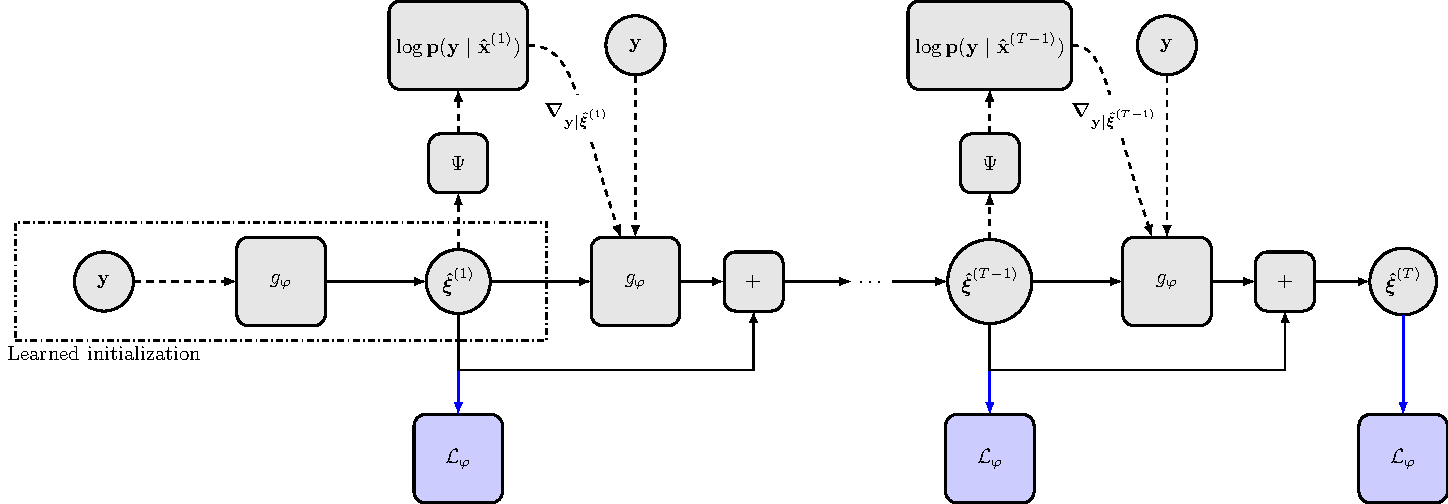
\includegraphics[width=\linewidth]{figures/schematic_rim_unrolled}
        \caption{Unrolled computational graph of the RIM. Operations along solid arrows are being 
        recorded for BPTT, while operations along dashed arrows are not. The blue arrows are only 
        used for optimisation during training. During fine-tuning or testing, the loss is computed only 
        as an oracle metric to validate that our methods can recover the ground truth.}
        \label{fig:unrolled graph}
\end{figure}
\begin{table}[H]
        \centering
        \caption{Hyperparameters for the RIM.}
        \label{tab:baseline hparams}
        \begin{tabular}{cc}
                Parameter & Value \\\hline\hline
                Source link function & $\bbone$ \\
                $\kappa$ link function & $10^{\boldsymbol{\xi}}$ \\
                                       & \\
                \textit{Architecture} & Figure \ref{fig:unet} \\
                Recurrent steps ($T$) & 8 \\
                Number of parameters & $348\,546\,818$ \\
                                      & \\
                \textit{First Stage Optimisation} & \\
                Optimizer & Adamax \\
                Initial learning rate & $10^{-4}$\\
                Learning rate schedule & Exponential Decay \\
                Decay rate & 0.95 \\
                Decay steps & $100\,000$\\
                Number of steps & $610\,000$\\
                Batch size & 1 \\
                           & \\
                \textit{Second Stage Optimisation} & \\
                Optimizer & Adamax \\
                Initial learning rate & $6\times 10^{-5}$\\
                Learning rate schedule & Exponential Decay \\
                Decay rate & 0.9 \\
                Decay steps & $100\,000$\\
                Number of steps & $870\,000$\\
                Batch size & 1 \\
                
                \hline
        \end{tabular}
\end{table}


%\begin{figure}[H]
        %\centering
        %\begin{tikzpicture}
                %\tikzstyle{every node}=[font=\scriptsize]
                %\node at (0, 0) {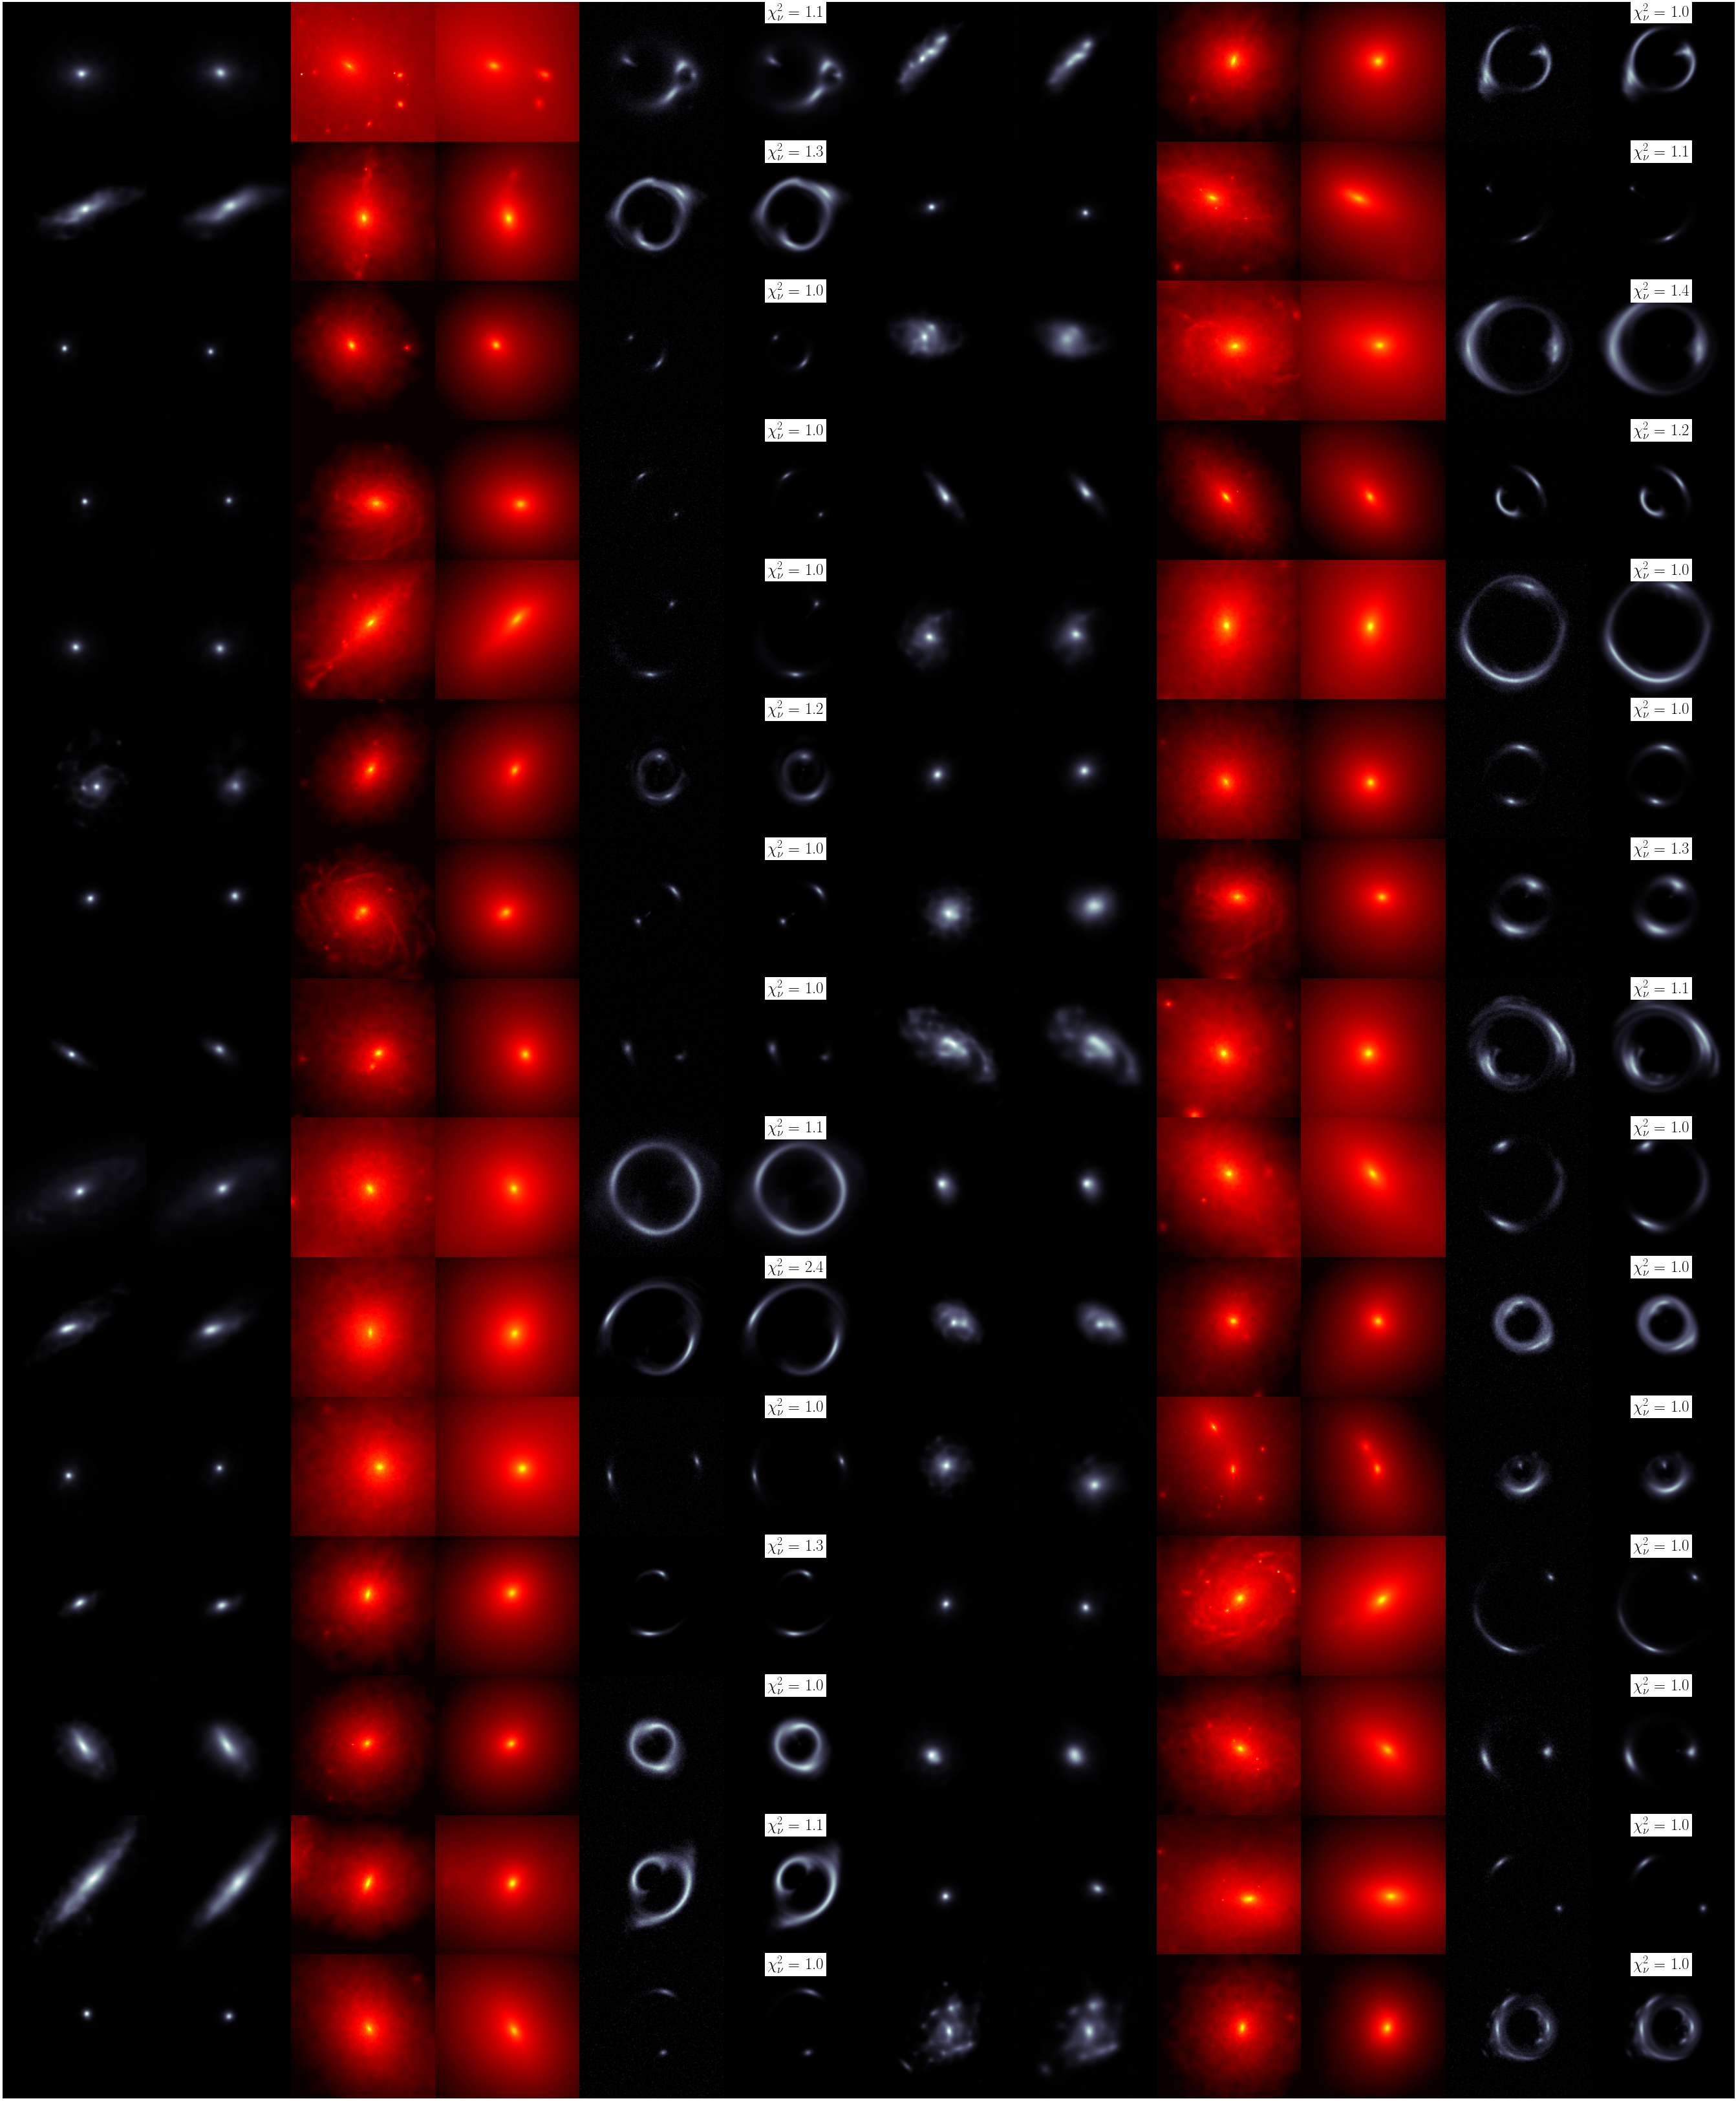
\includegraphics[width=\linewidth]{figures/test_set_no_cherry_pick}};
                %\node at (-8.2, 11) {COSMOS\strut};
                %\node at (-6.8, 11) {RIM+FT\strut};
                %\node at (-5.3, 11) {IllustrisTNG\strut};
                %\node at (-3.7, 11) {RIM+FT\strut};
                %\node at (-2.2, 11) {Observation\strut};
                %\node at (-0.8, 11) {RIM+FT\strut};

                %\node at (0.6, 11) {COSMOS\strut};
                %\node at (2.1, 11) {RIM+FT\strut};
                %\node at (3.7, 11) {IllustrisTNG\strut};
                %\node at (5.2, 11) {RIM+FT\strut};
                %\node at (6.7, 11) {Observation\strut};
                %\node at (8.2, 11) {RIM+FT\strut};

                
                %% \node at (-7.5, 11.2) {COSMOS};
                %% \node at (-4.5, 11.2) {RIM+FT};
                %% \node at (-6, 11.7) {Sources};
                %% \node at (-1.5, 11.2) {Illustris TNG};
                %% \node at (1.5, 11.2) {RIM+FT};
                %% \node at (0, 11.7) {Convergence};
                %% \node at (4.5, 11.2) {Observation};
                %% \node at (7.5, 11.2) {RIM+FT};
        %\end{tikzpicture}
        %\caption{
                %30 reconstructions taken at random from the test set of 3000 examples simulated from COSMOS 
                %and IllustrisTNG data at high SNR.
                %The colorscale are the same as in Figure \ref{fig:main result}.}
        %\label{fig:random sample}
%\end{figure}


  \chapter{GRU}\label{ap:gru}
Une unité récurrente à porte convolutionnelles est décrite par les opérations
\begin{align}
		\tilde{\mathbf{x}} &= S\bigg( \mathbf{w}_o * (\mathbf{h}^{(t-1)} \oplus \mathbf{x}^{(t)}) + \mathbf{b}_o\bigg) &\{\text{Porte d'oubli}\} \\
		\mathbf{z} &= S\bigg( \mathbf{w}_z * (\mathbf{h}^{(t-1)} \oplus \mathbf{x}^{(t)}) + \mathbf{b}_{z}\bigg)&\{\text{Porte de mise à jour}\} \\
		\tilde{\mathbf{h}} &= \tanh\bigg( \mathbf{w}_h * \big((\mathbf{h}^{(t-1)}\odot \tilde{\mathbf{x}}) \oplus \mathbf{x}^{(t)})\big) + \mathbf{b}_{h}\bigg)&\{\text{État candidat}\} \\
	\label{eq:nouvel etat}
		\mathbf{h}^{(t)} &=\mathbf{h}^{(t-1)} \odot \mathbf{z} + \tilde{\mathbf{h}} \odot (1 - \mathbf{z}) &\{\text{Nouvel état}\} 
\end{align}
où $S(x) = \frac{1}{1 + e^{-x}}$ est une fonction sigmoïde et $\mathbf{x}^{(t)}$ est un tenseur à l'entrée de l'unité. 
Les noyaux de convolution $\mathbf{w}$ et les vecteurs de biais $\mathbf{b}$  
sont des paramètres libres appris par descente de gradient stochastique. $\oplus$ symbolise l'opération 
de concatenation. Le tenseur de sortie de cette unité, soit le nouvel état latent $\mathbf{h}^{(t)}$, 
est une combinaison de l'état latent précédent $\mathbf{h}^{(t-1)}$ et de l'état candidat 
$\tilde{\mathbf{h}}$, pesée élément par élément par le vecteur à la sortie de la porte de mise à jour $\mathbf{z}$.



  %\printbibliography[heading=bibintoc]
\end{document}

